\clearpage
\appendix 
%%%%%%%%%%%%%%%%%%%%%%%%%%%%%%%%%%%%%%%%%%%%%%%%%%%%%%%%%%%%%%

\section{Analyzing Deep Neural Networks}
Here we visualize different Network semantic maps generated during our analysis. In the 1D case we fix the elevation of the camera to a nominal angle of $\ang{35}$ and rotate around the object. In the 2D case, we change both the elevation and azimuth around the object. These maps can be generated to any type of semantic parameters that affect the generation of the image , and not viewing angle. 
\subsection{Networks Semantic Maps (1D)}
In \figLabel{\ref{fig:nsm1d-1},\ref{fig:nsm1d-2}} we visualize the 1D semantic maps of rotating around the object and recording different DNNs performance and averaging the profile over 10 different shapes per class.

\begin{figure*}[h]
\centering
\tabcolsep=0.03cm
   \begin{tabular}{c|c}
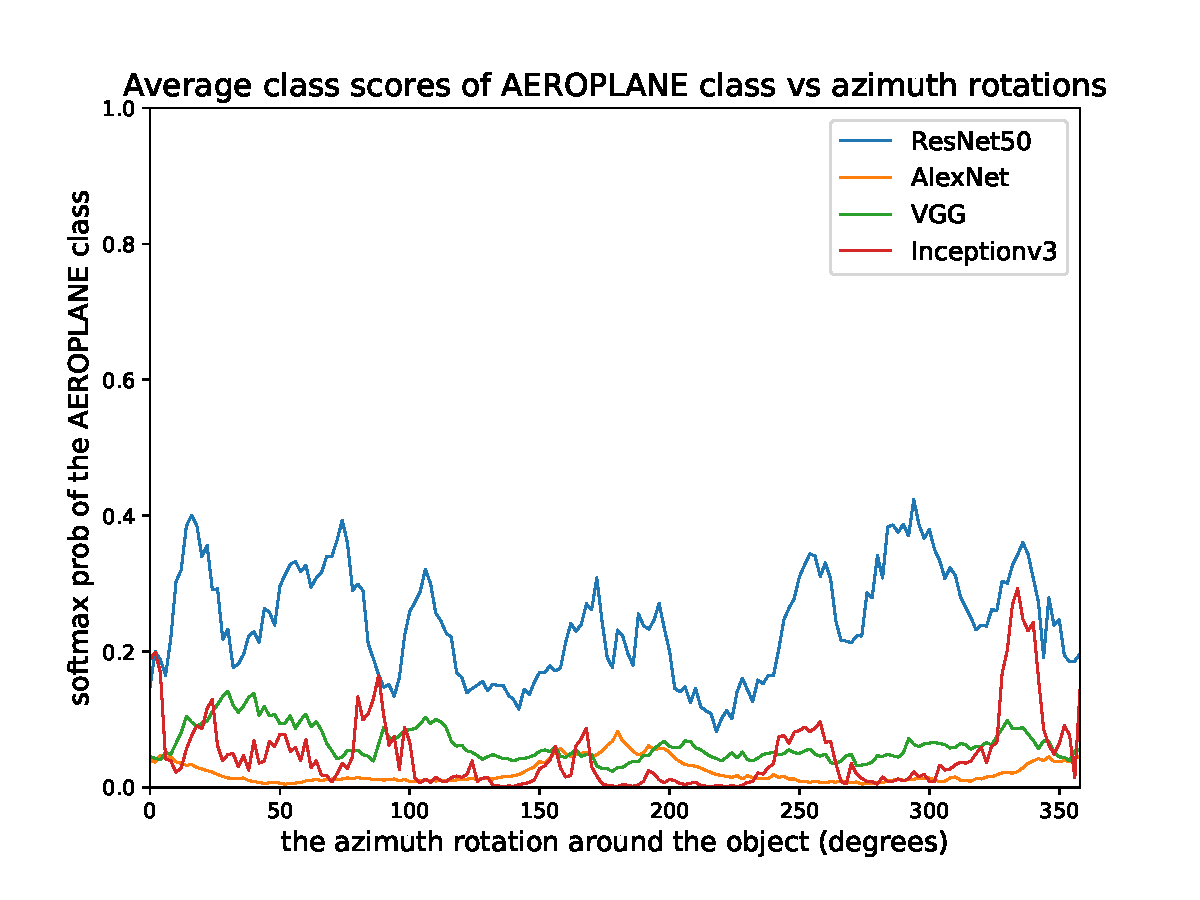
\includegraphics[width = 9cm]{supimages/nms1d/average_azimuth_performance_AEROPLANE.pdf}&
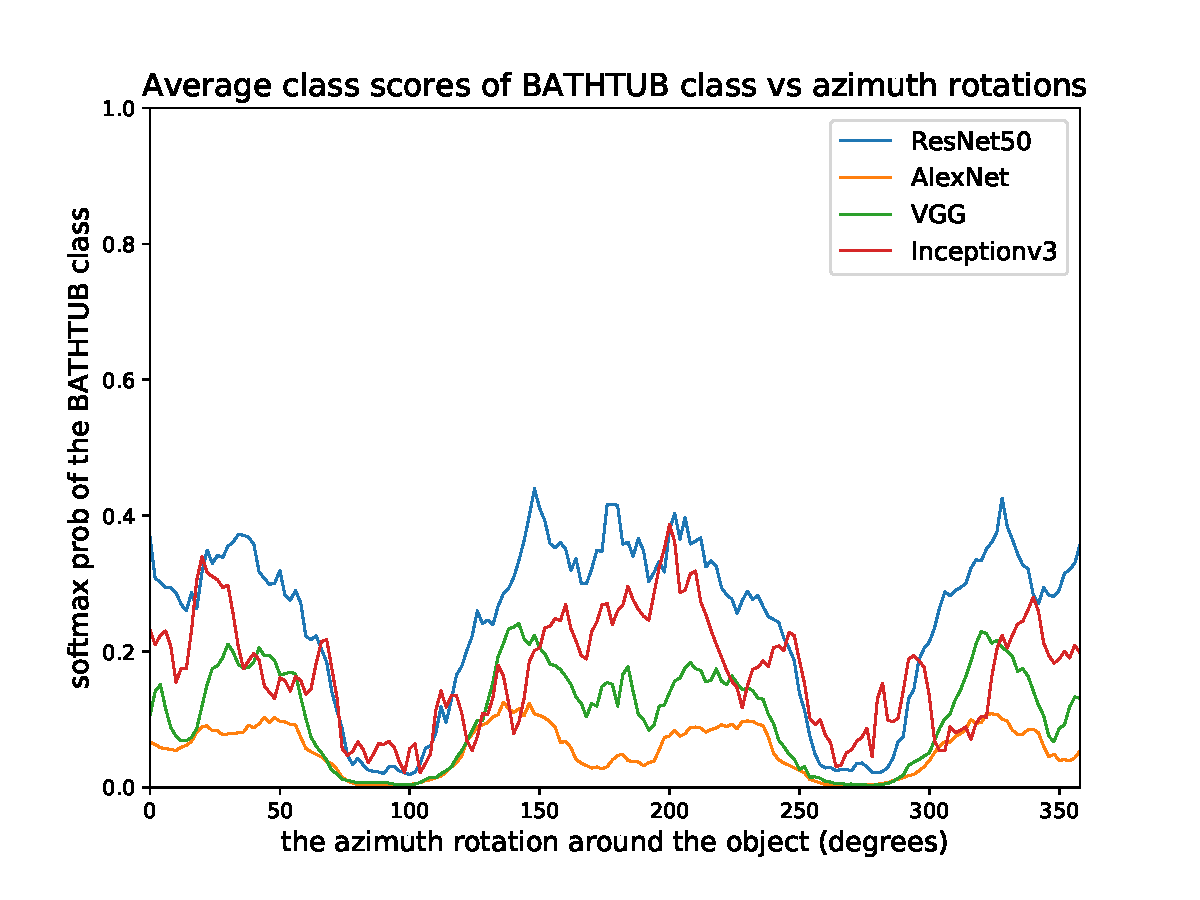
\includegraphics[width = 9cm]{supimages/nms1d/average_azimuth_performance_BATHTUB.pdf}\\ \hline
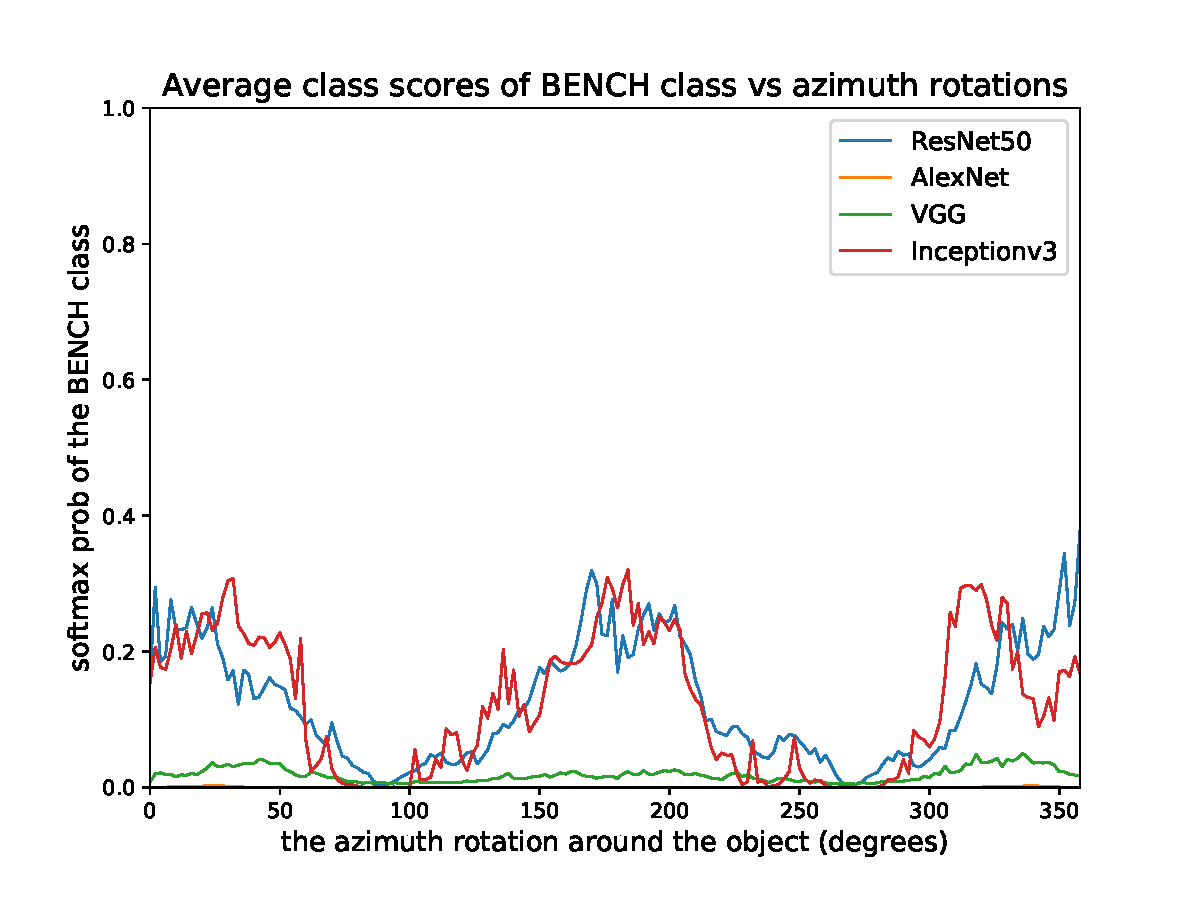
\includegraphics[width = 9cm]{supimages/nms1d/average_azimuth_performance_BENCH.pdf}&
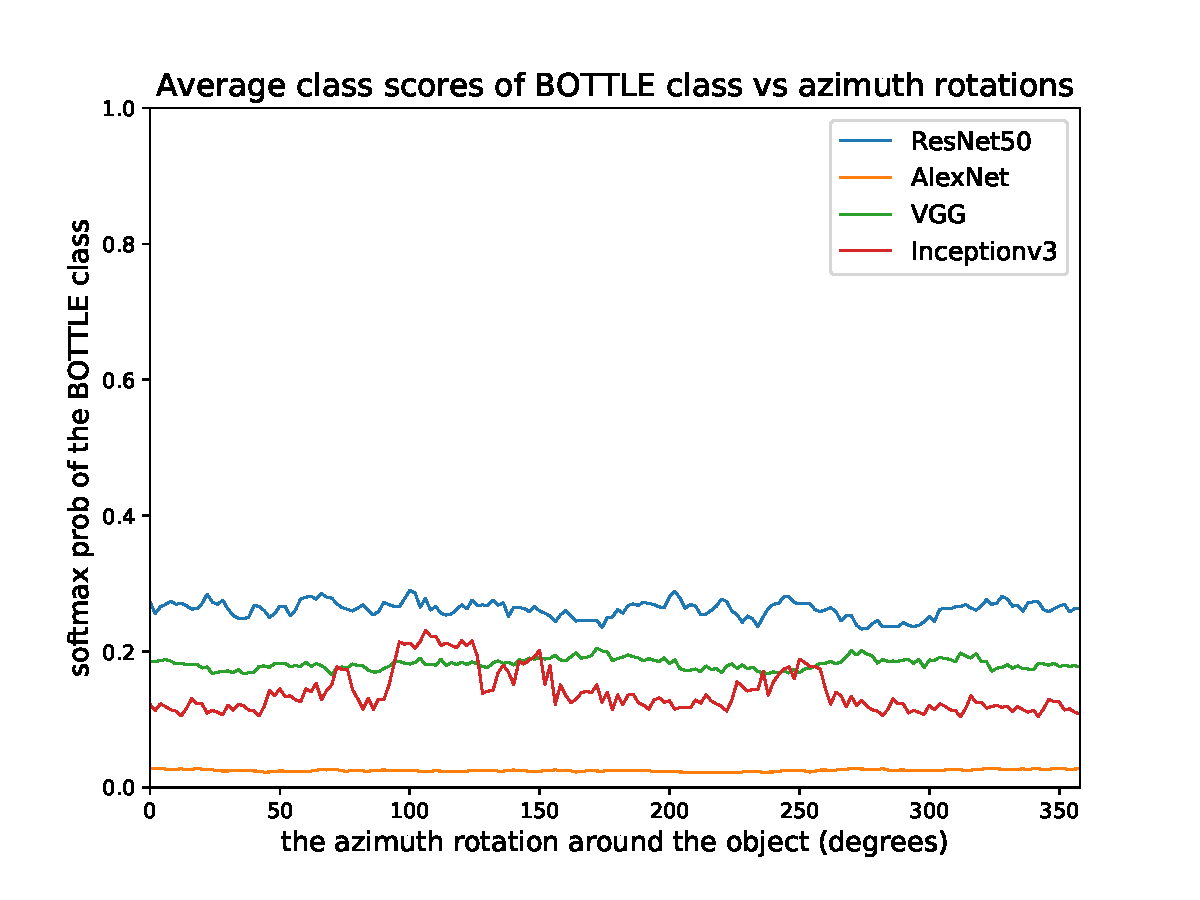
\includegraphics[width = 9cm]{supimages/nms1d/average_azimuth_performance_BOTTLE.pdf}
% 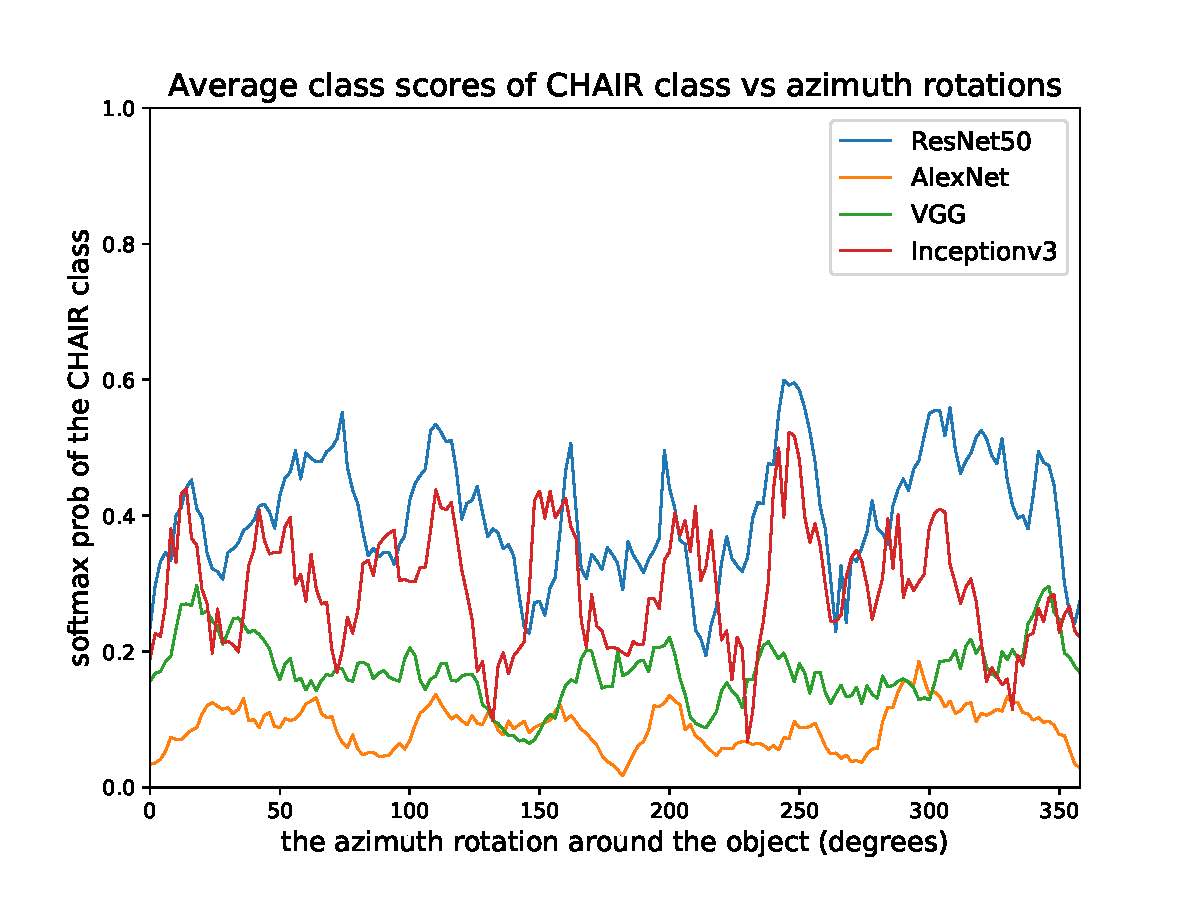
\includegraphics[width = 9cm]{supimages/nms1d/average_azimuth_performance_CHAIR.pdf}&
% 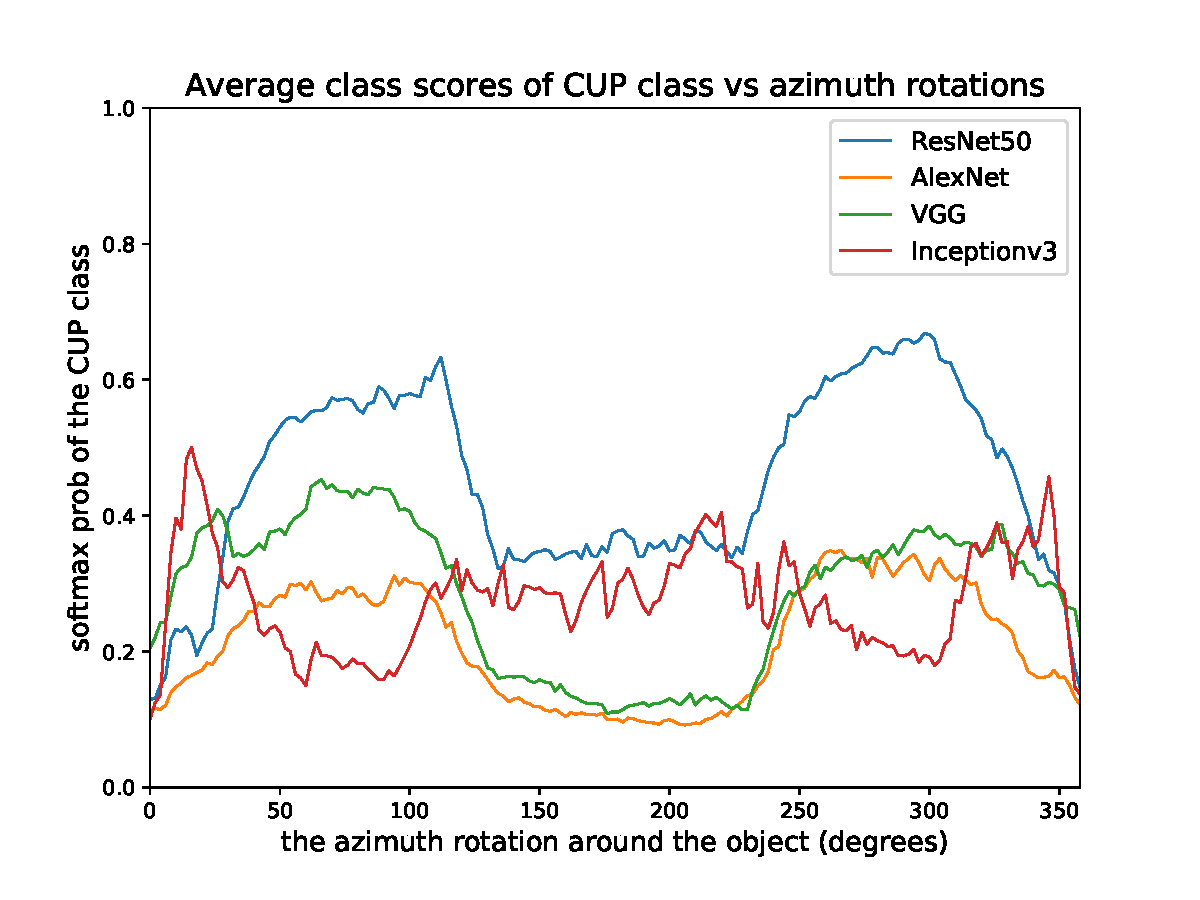
\includegraphics[width = 9cm]{supimages/nms1d/average_azimuth_performance_CUP.pdf}\\
% 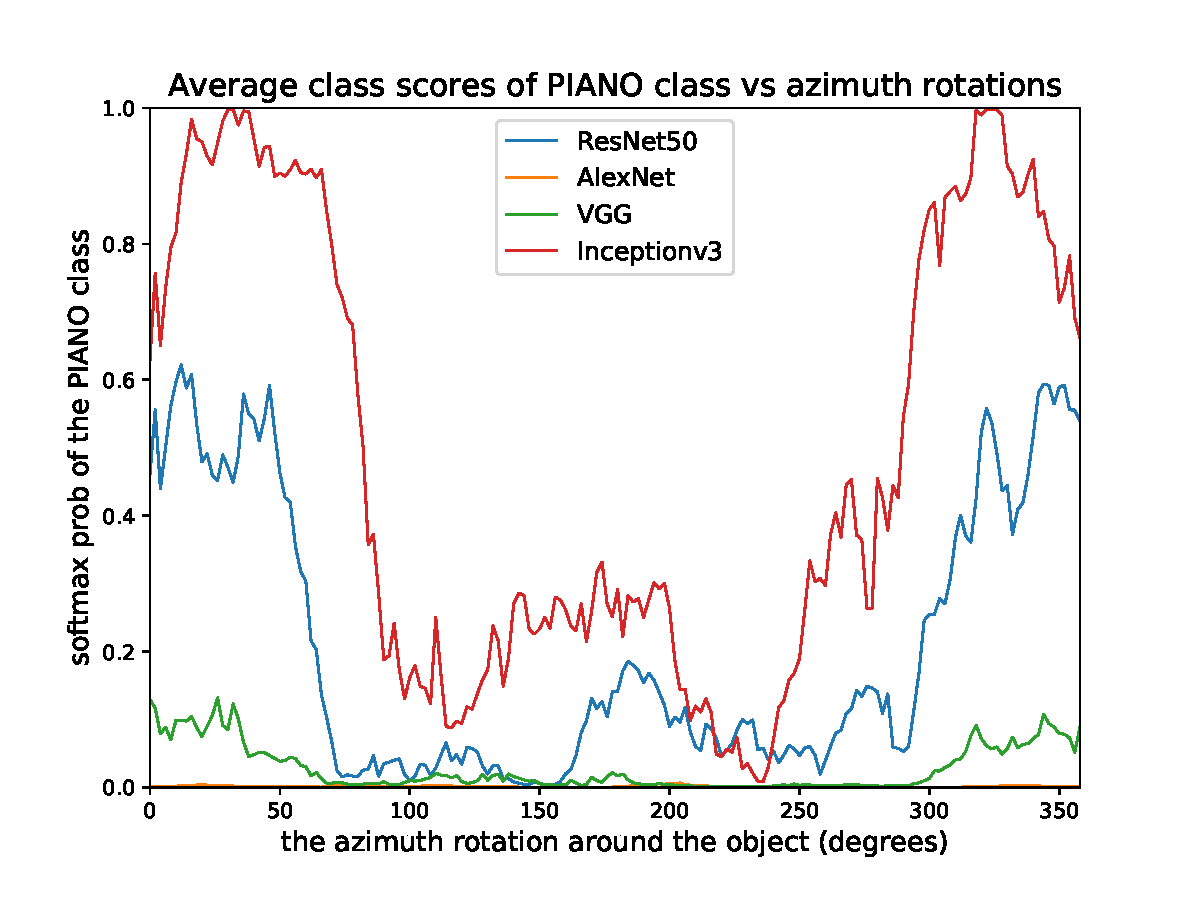
\includegraphics[width = 9cm]{supimages/nms1d/average_azimuth_performance_PIANO.pdf}&
% 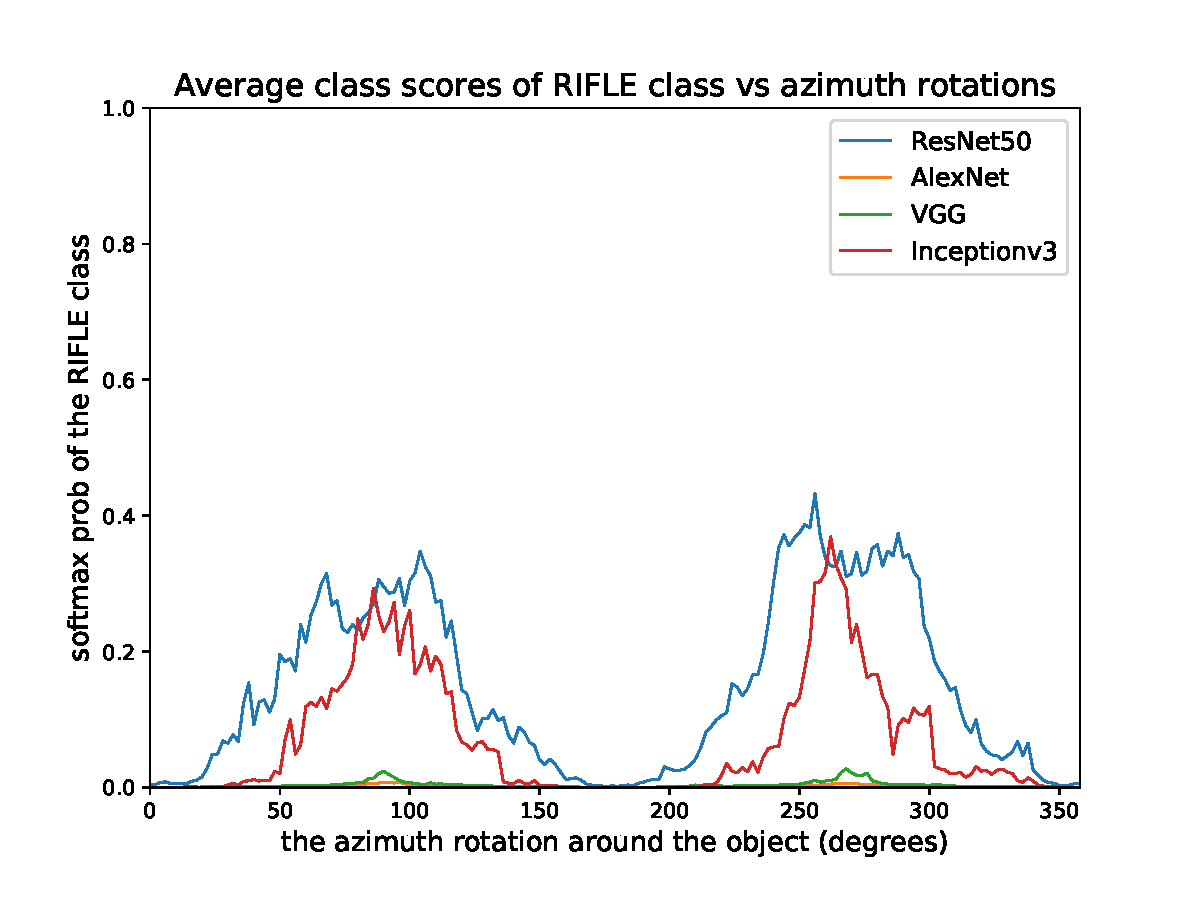
\includegraphics[width = 9cm]{supimages/nms1d/average_azimuth_performance_RIFLE.pdf}\\
% 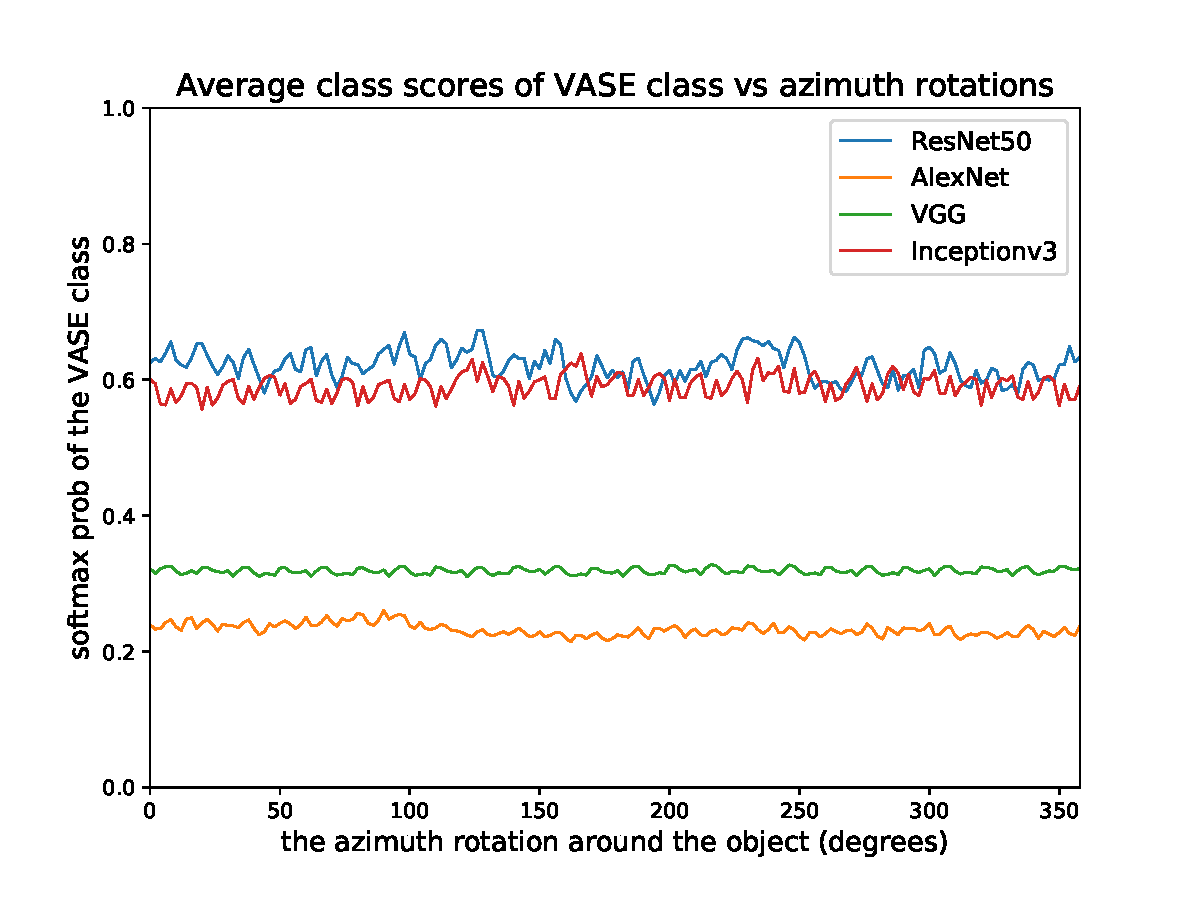
\includegraphics[width = 9cm]{supimages/nms1d/average_azimuth_performance_VASE.pdf}&
% \includegraphics[width = 9cm]{supimages/nms1d/average_azimuth_performance_TOILET.pdf}
\end{tabular}
    %   \vspace{-9pt}
   \caption{\small \textbf{1D Network Semantic Maps NMS-I}: visualizing 1D Semantic Robustness profile for different networks averaged over 10 different shapes. Observe that different DNNs profiles differ depending on the training , accuracy , and network architectures that all result in a unique ''signatures" for the DNN on that class. The correlation between the DNN profiles is due to the common data bias in ImageNet.}
   \vspace{-8pt}
   \label{fig:nsm1d-1}
\end{figure*}

\begin{figure*}[h]
\centering
\tabcolsep=0.03cm
   \begin{tabular}{c|c}
% 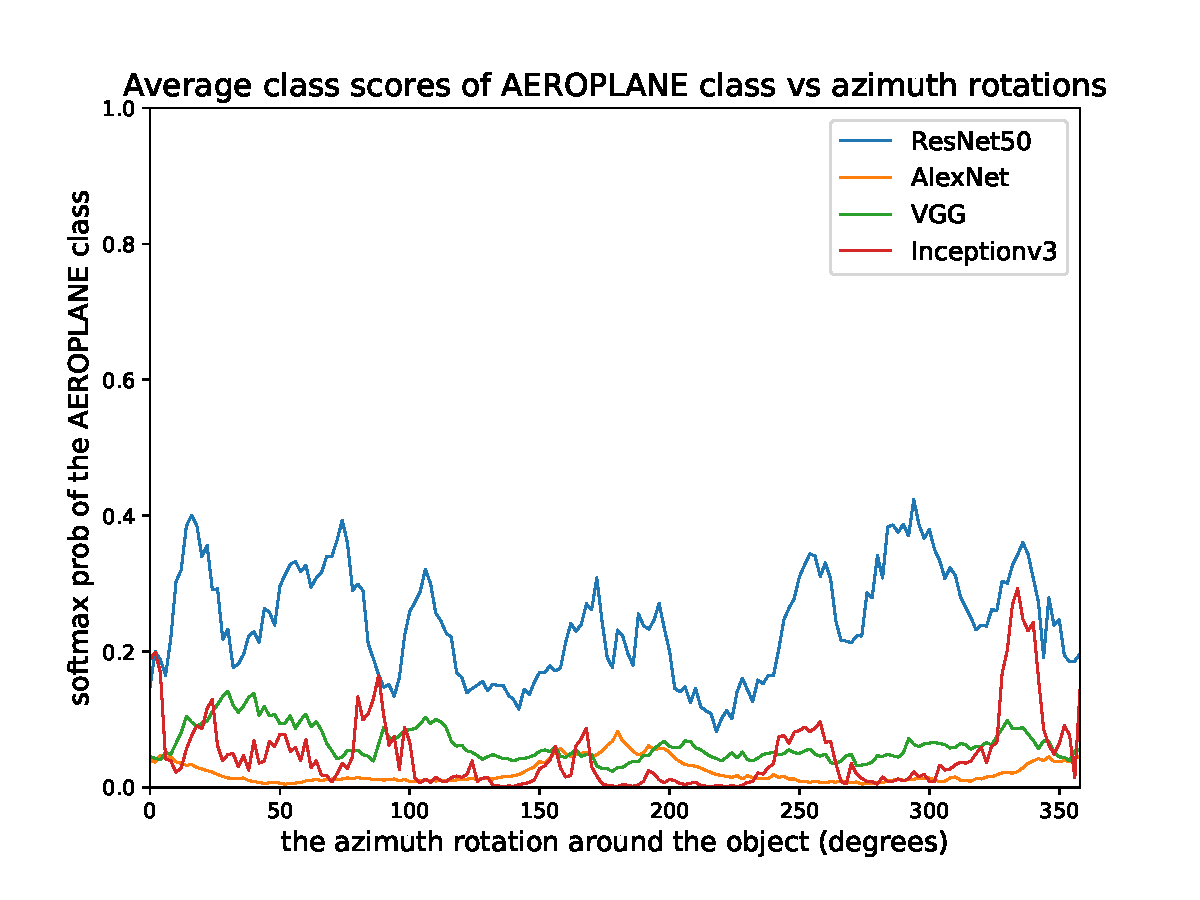
\includegraphics[width = 9cm]{supimages/nms1d/average_azimuth_performance_AEROPLANE.pdf}&
% 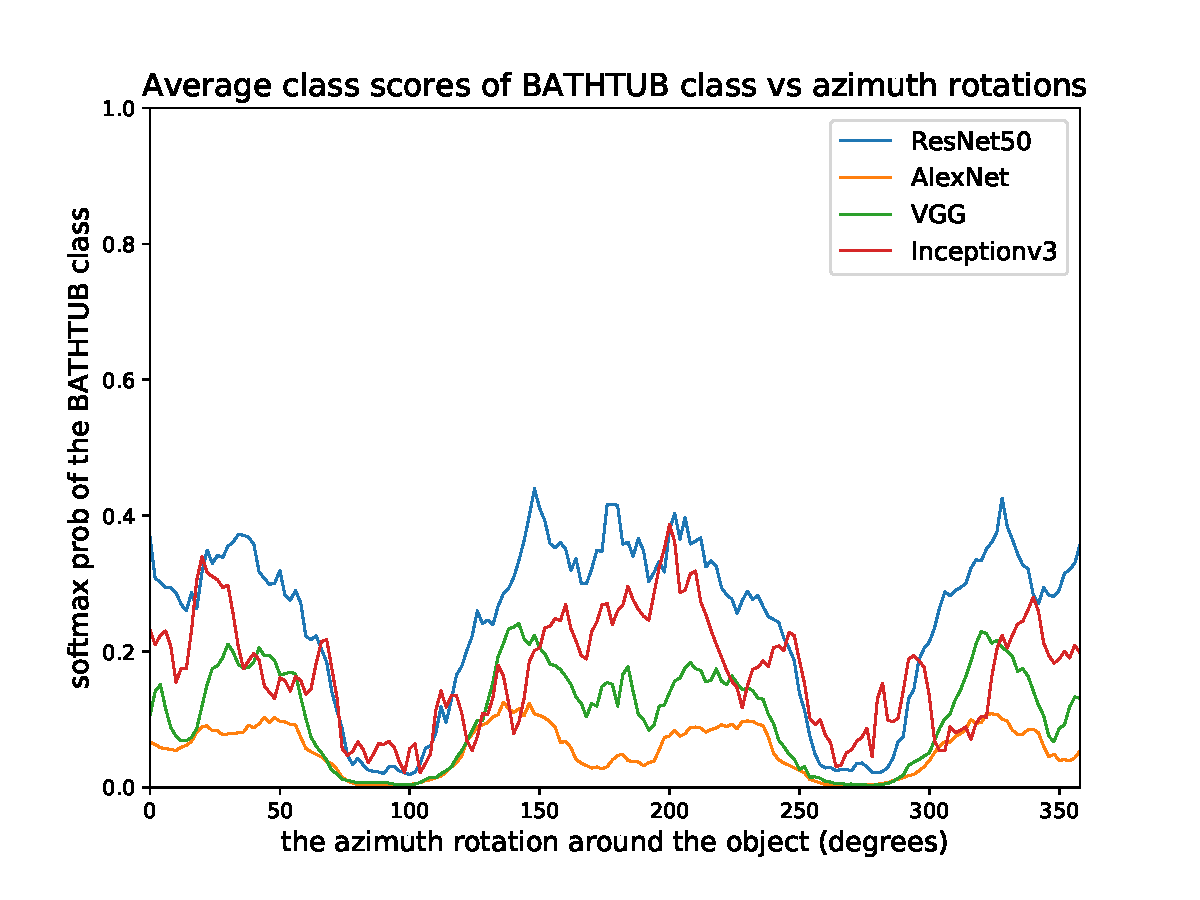
\includegraphics[width = 9cm]{supimages/nms1d/average_azimuth_performance_BATHTUB.pdf}\\
% 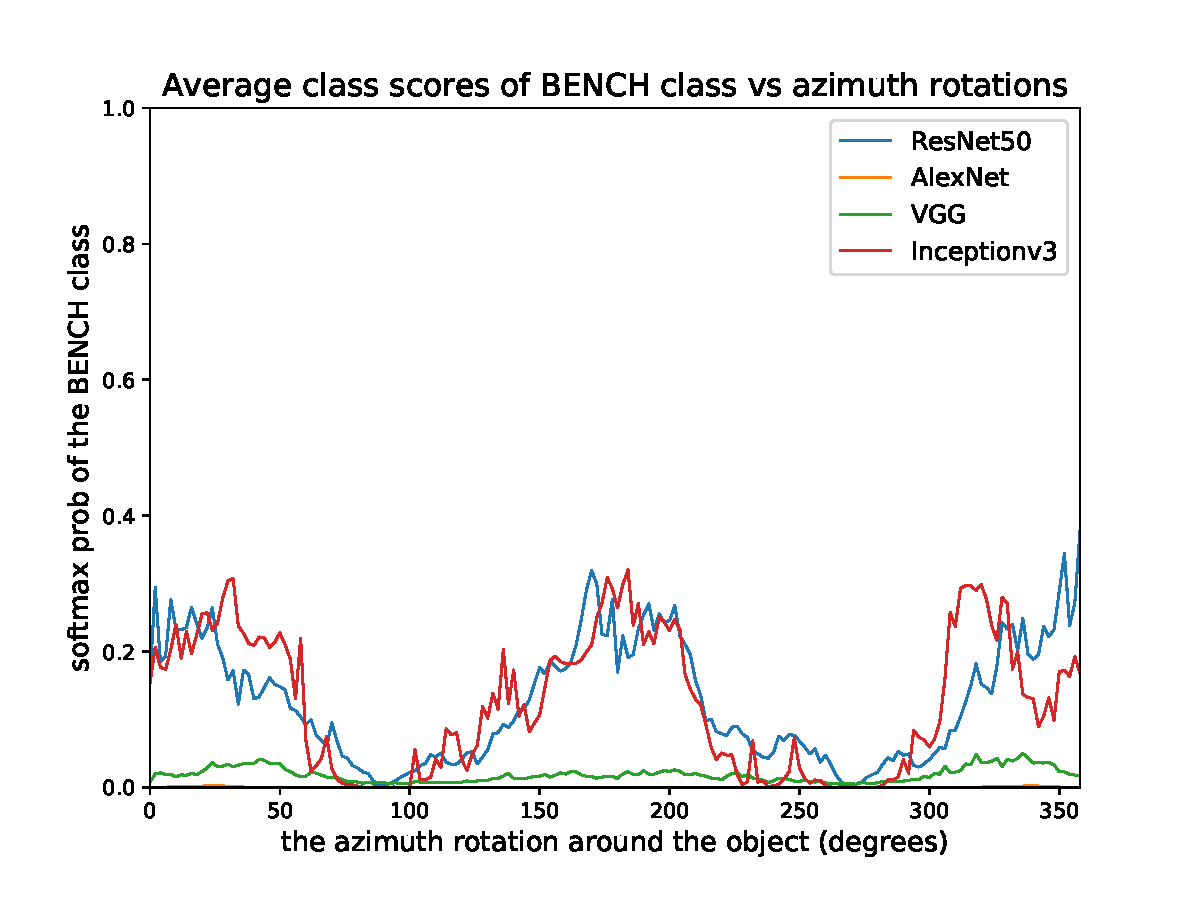
\includegraphics[width = 9cm]{supimages/nms1d/average_azimuth_performance_BENCH.pdf}&
% 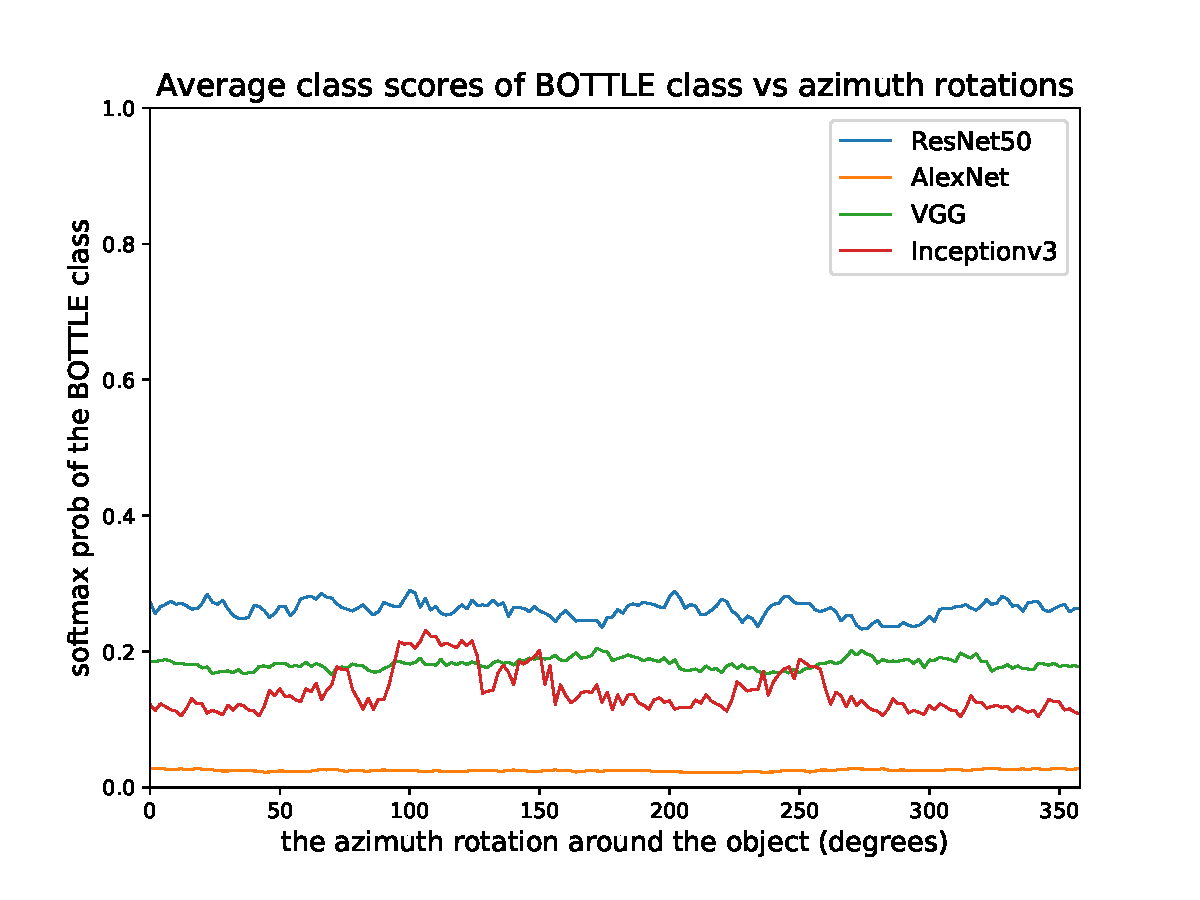
\includegraphics[width = 9cm]{supimages/nms1d/average_azimuth_performance_BOTTLE.pdf}\\
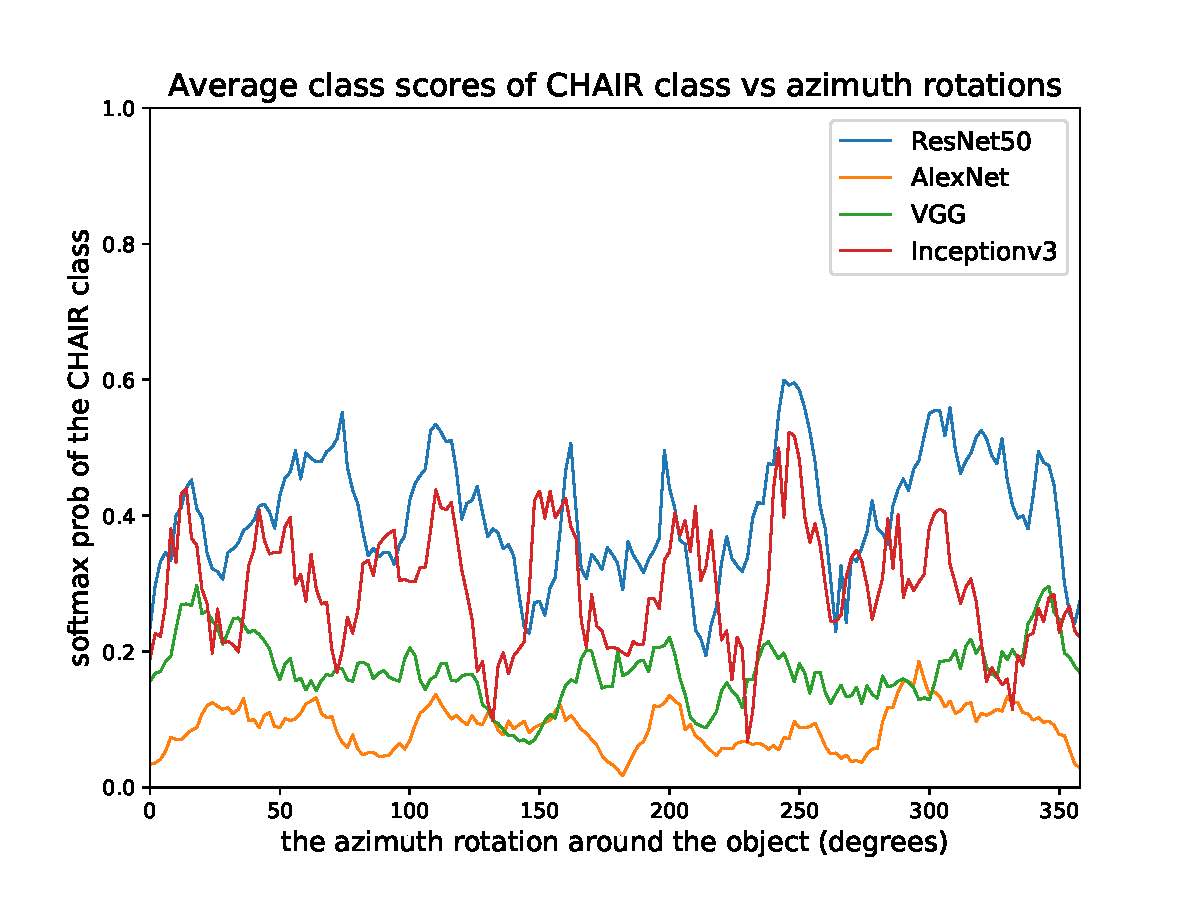
\includegraphics[width = 9cm]{supimages/nms1d/average_azimuth_performance_CHAIR.pdf}&
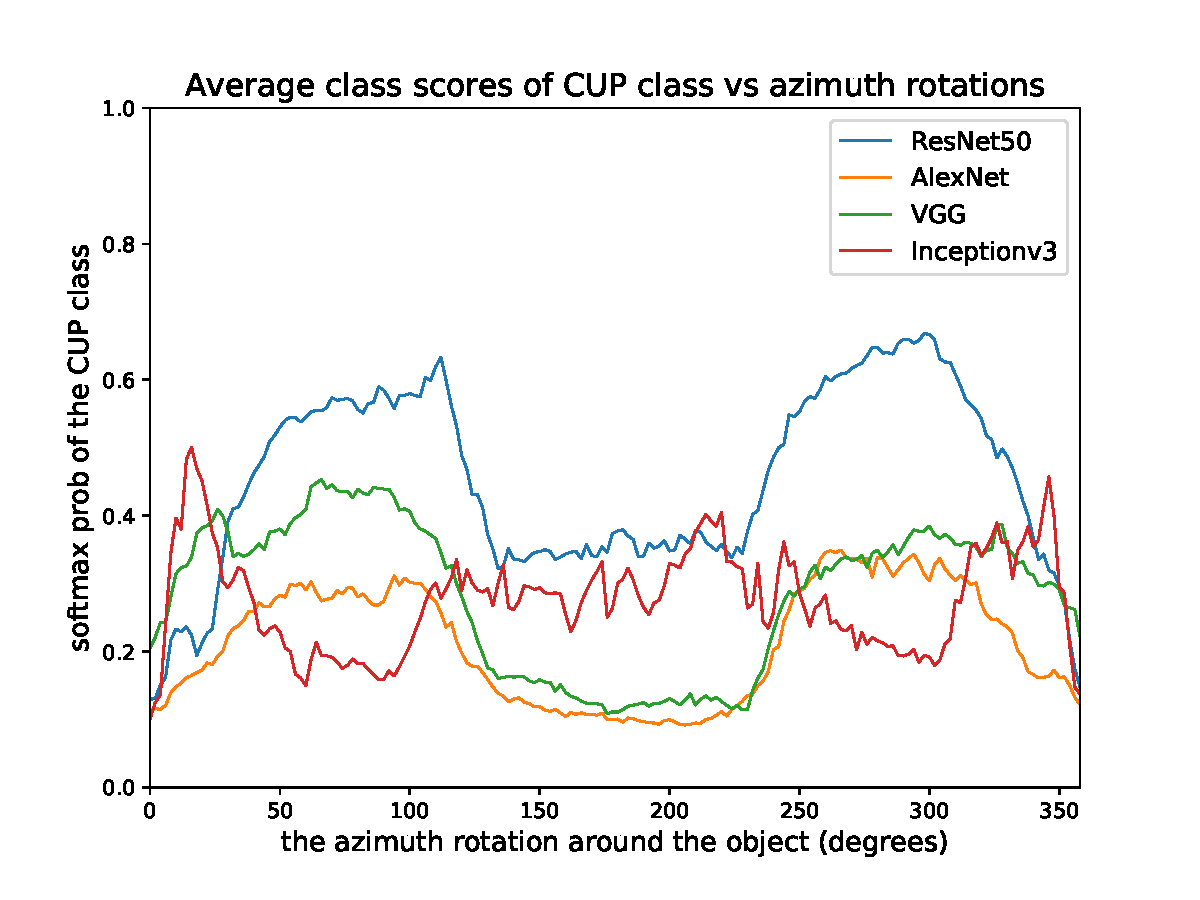
\includegraphics[width = 9cm]{supimages/nms1d/average_azimuth_performance_CUP.pdf}\\\hline
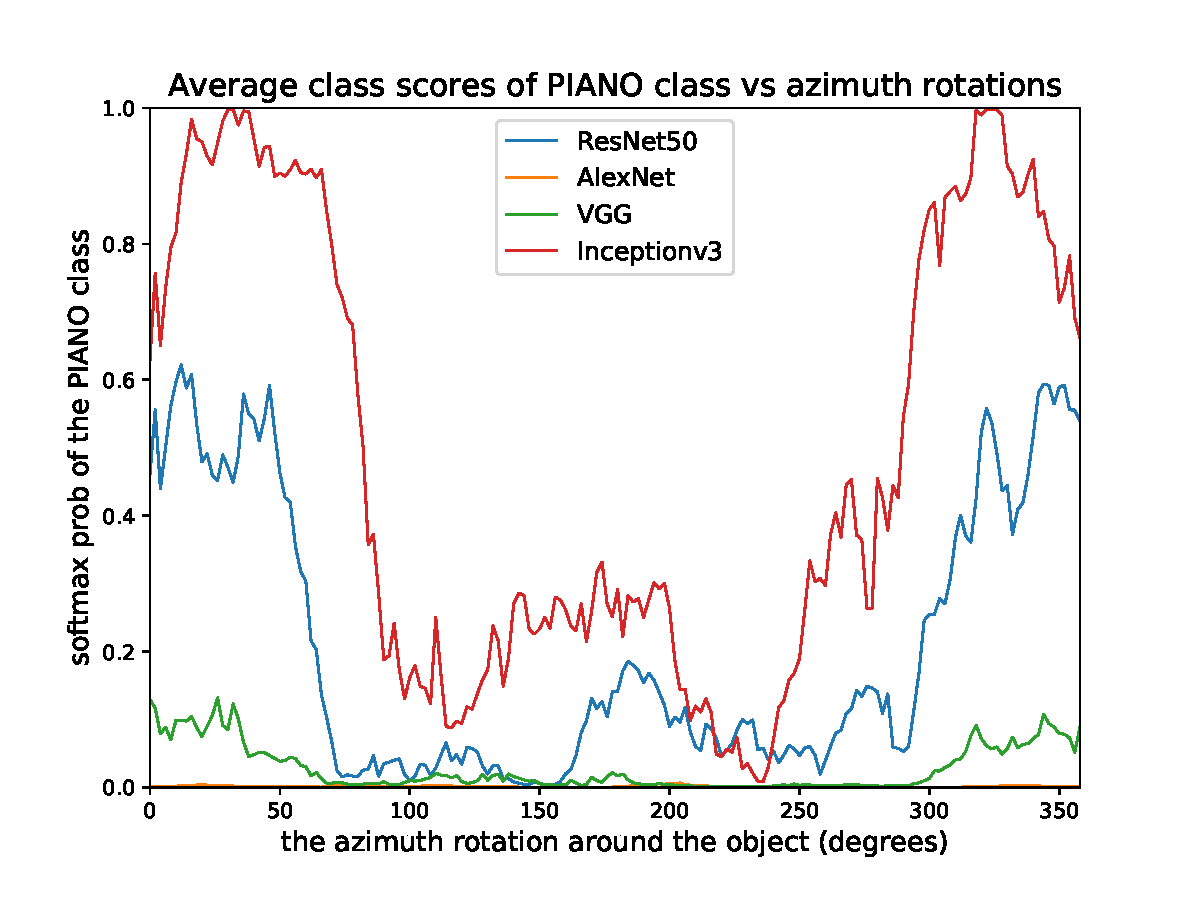
\includegraphics[width = 9cm]{supimages/nms1d/average_azimuth_performance_PIANO.pdf}&
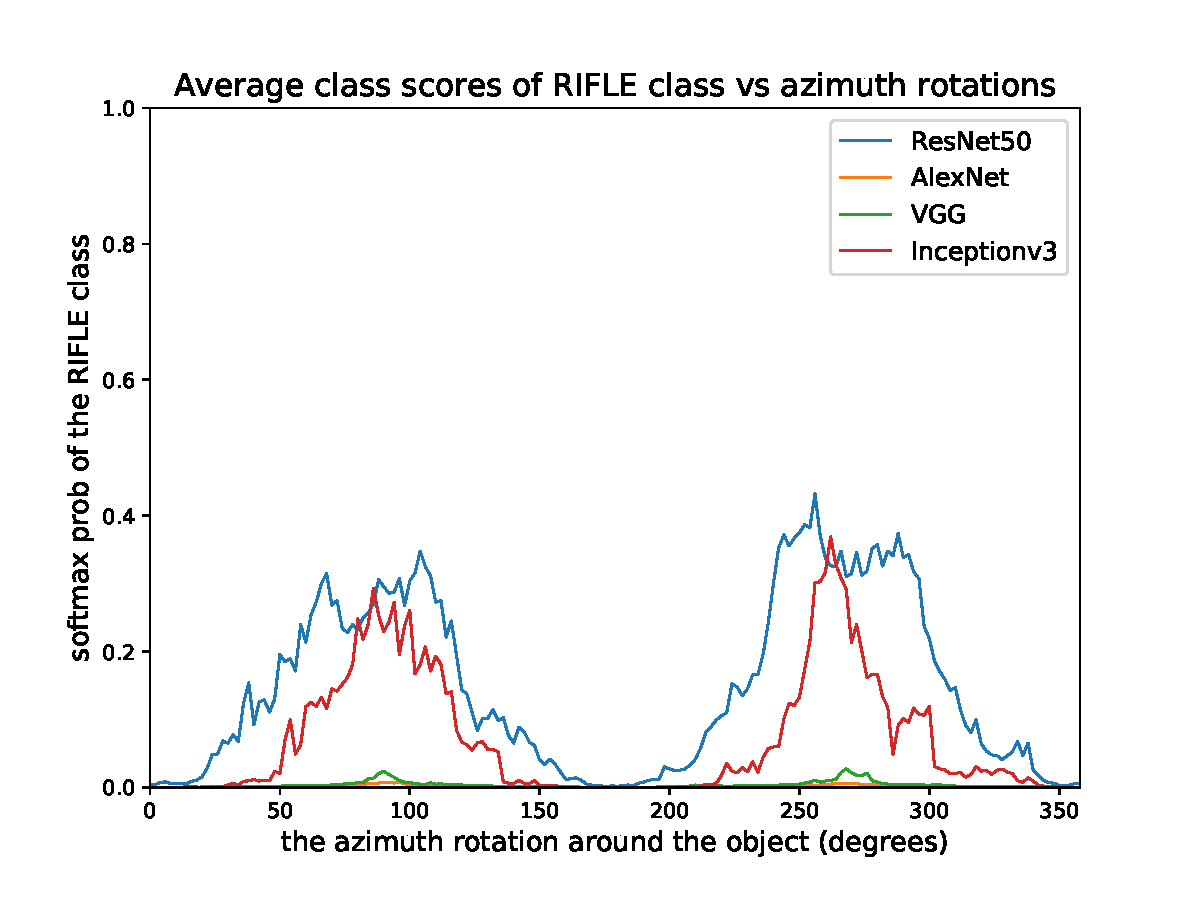
\includegraphics[width = 9cm]{supimages/nms1d/average_azimuth_performance_RIFLE.pdf}\\\hline
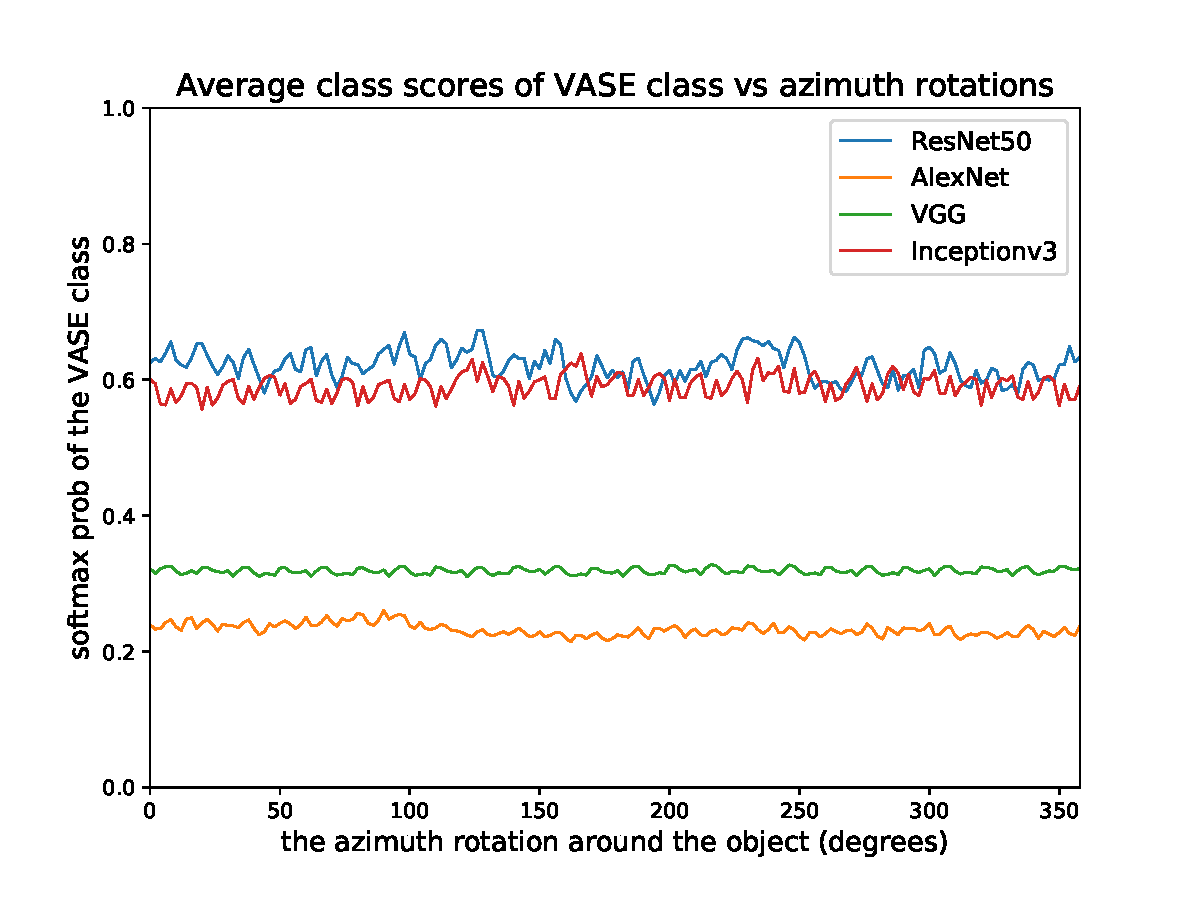
\includegraphics[width = 9cm]{supimages/nms1d/average_azimuth_performance_VASE.pdf}&
\includegraphics[width = 9cm]{supimages/nms1d/average_azimuth_performance_TOILET.pdf}
\end{tabular}
    %   \vspace{-9pt}
   \caption{\small \textbf{1D Network Semantic Maps NMS-II}: visualizing 1D Semantic Robustness profile for different networks averaged over 10 different shapes. Observe that different DNNs profiles differ depending on the training , accuracy , and network architectures that all result in a unique ''signatures" for the DNN on that class. The correlation between the DNN profiles is due to the common data bias in ImageNet.}
   \vspace{-8pt}
   \label{fig:nsm1d-2}
\end{figure*}
% \clearpage

\subsection{Networks Semantic Maps (2D)}
In \figLabel{\ref{fig:nsm2d-1},\ref{fig:nsm2d-2}} we visualize the 2D semantic maps of elevation angles and rotating around the object and recording different DNNs performance and averaging the maps over 10 different shapes per class.
\begin{figure*}[h]
\centering
\tabcolsep=0.03cm
   \begin{tabular}{||c|c|c|c||} \hline
   \textbf{AlexNet} & \textbf{VGG} &\textbf{ResNet50} & \textbf{InceptionV3} \\ \hline
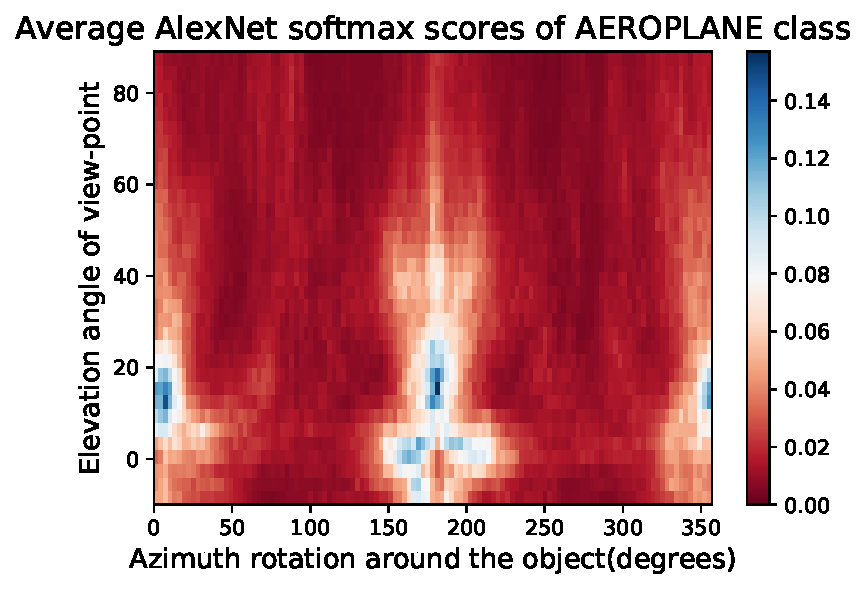
\includegraphics[width = 4cm]{supimages/nms2d/AlexNet_aeroplane_Average.pdf}&
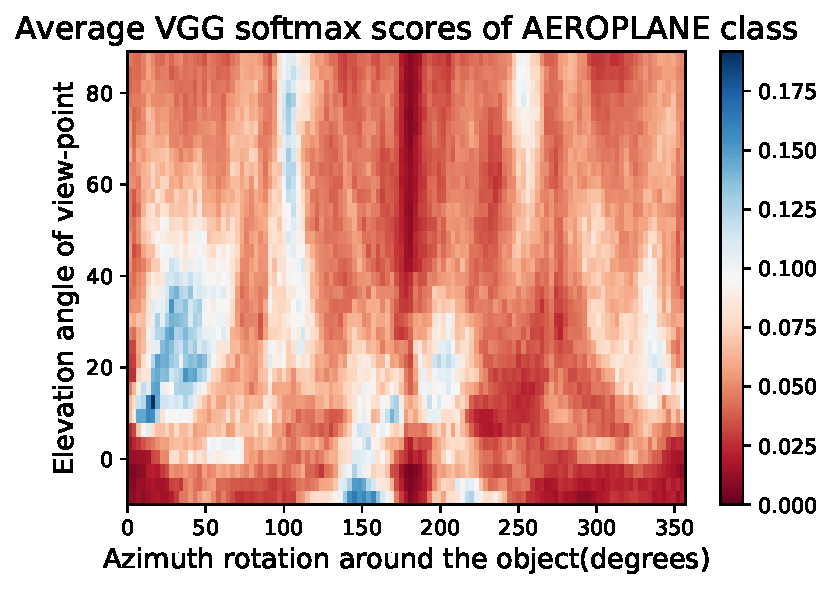
\includegraphics[width = 4cm]{supimages/nms2d/VGG_aeroplane_Average.pdf}&
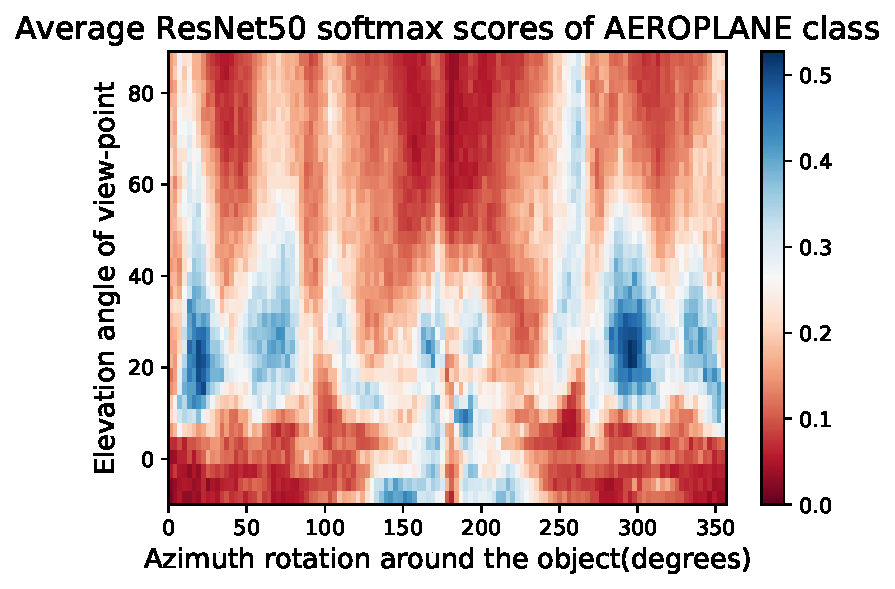
\includegraphics[width = 4cm]{supimages/nms2d/ResNet50_aeroplane_Average.pdf}&
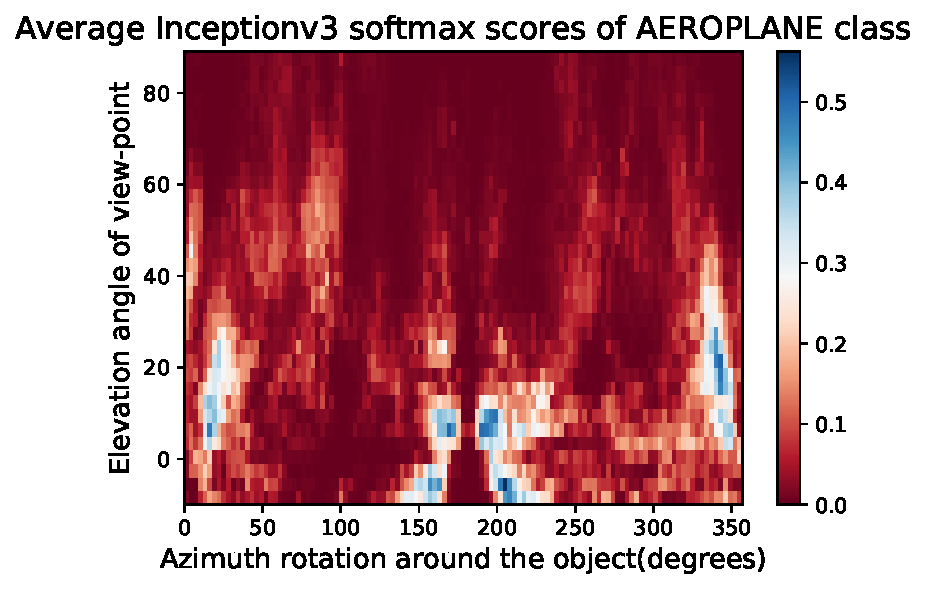
\includegraphics[width = 4cm]{supimages/nms2d/Inceptionv3_aeroplane_Average.pdf}\\ \hline
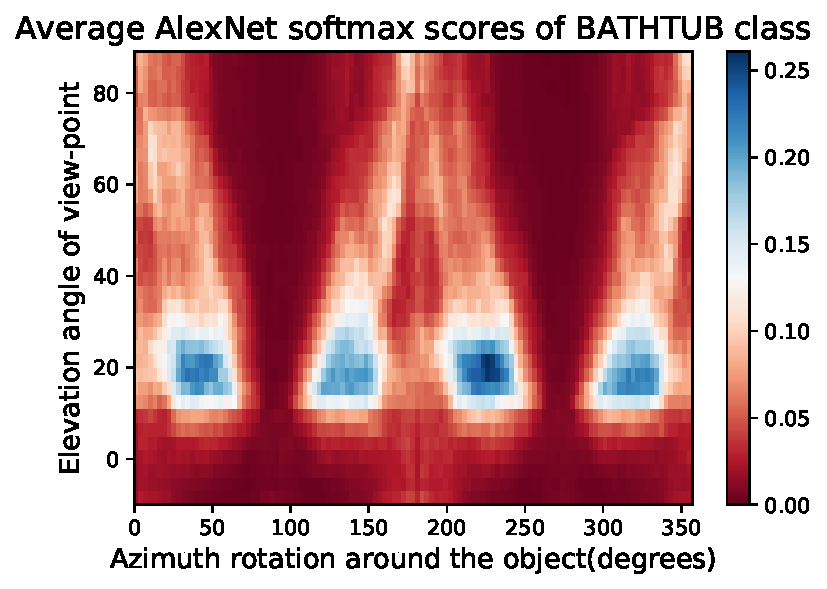
\includegraphics[width = 4cm]{supimages/nms2d/AlexNet_bathtub_Average.pdf}&
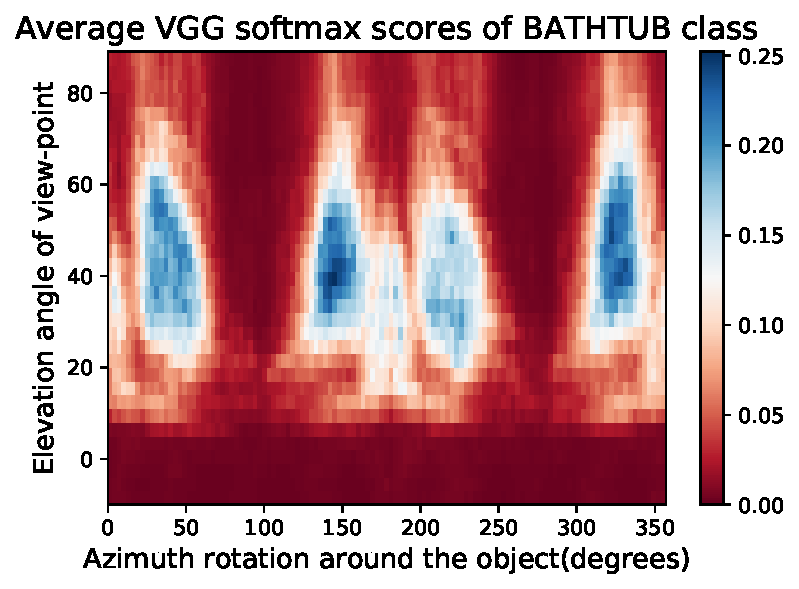
\includegraphics[width = 4cm]{supimages/nms2d/VGG_bathtub_Average.pdf}&
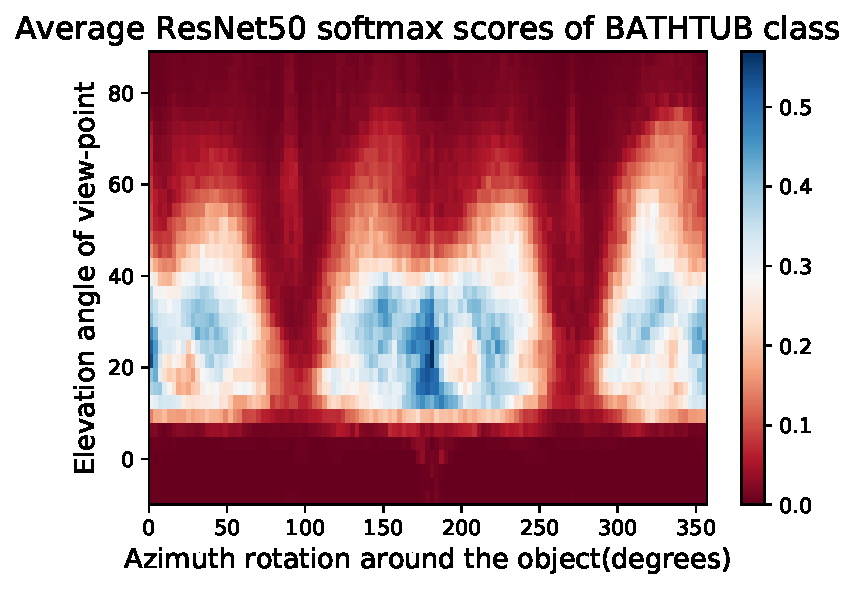
\includegraphics[width = 4cm]{supimages/nms2d/ResNet50_bathtub_Average.pdf}&
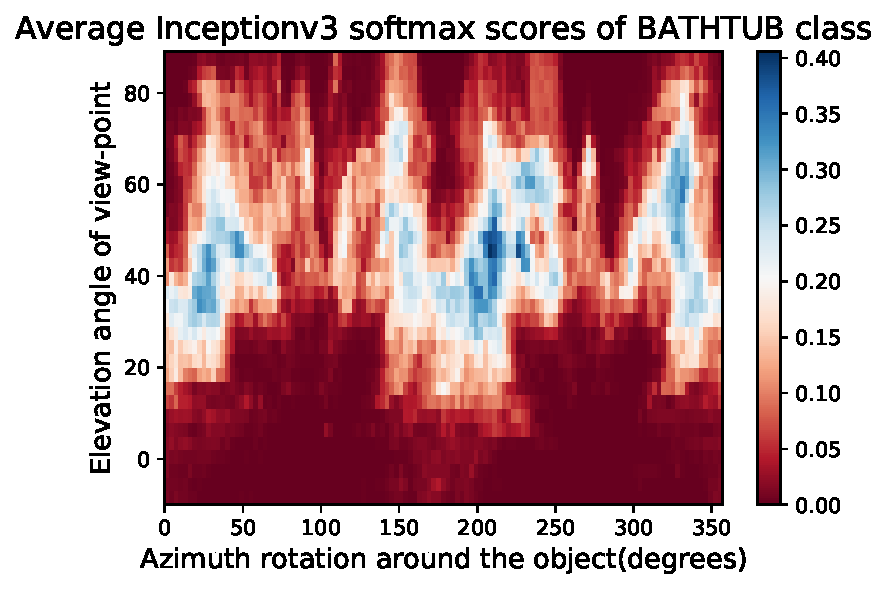
\includegraphics[width = 4cm]{supimages/nms2d/Inceptionv3_bathtub_Average.pdf}\\ \hline
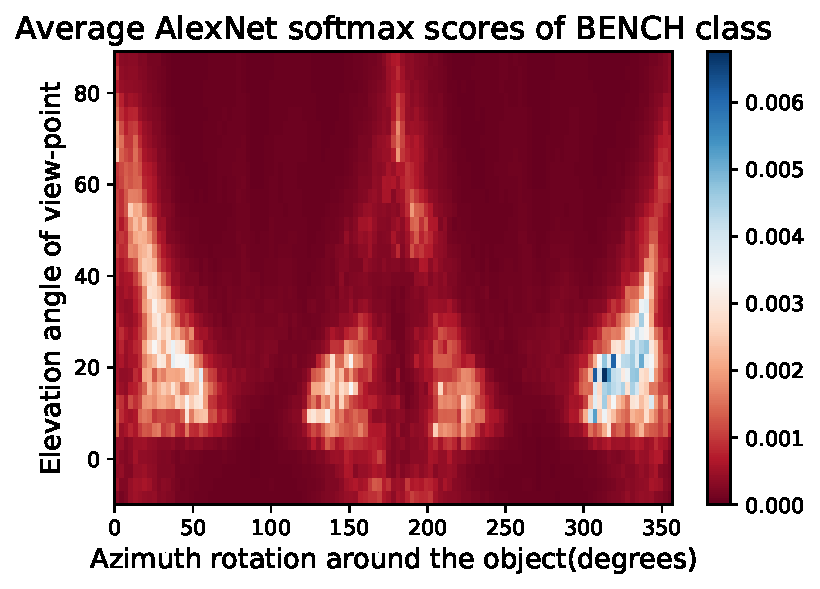
\includegraphics[width = 4cm]{supimages/nms2d/AlexNet_bench_Average.pdf}&
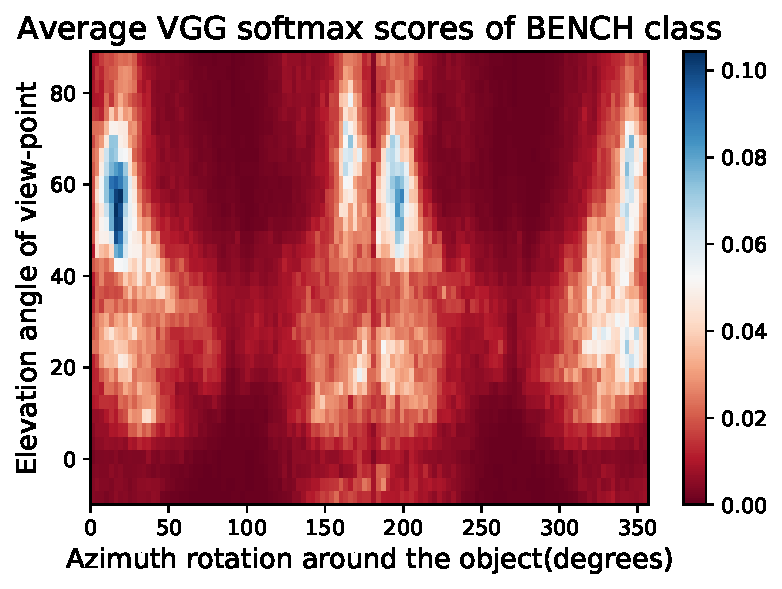
\includegraphics[width = 4cm]{supimages/nms2d/VGG_bench_Average.pdf}&
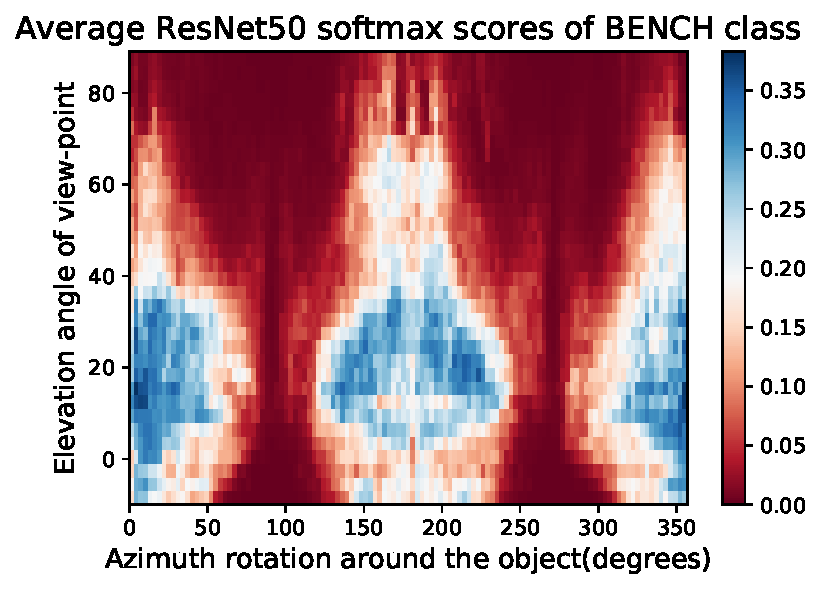
\includegraphics[width = 4cm]{supimages/nms2d/ResNet50_bench_Average.pdf}&
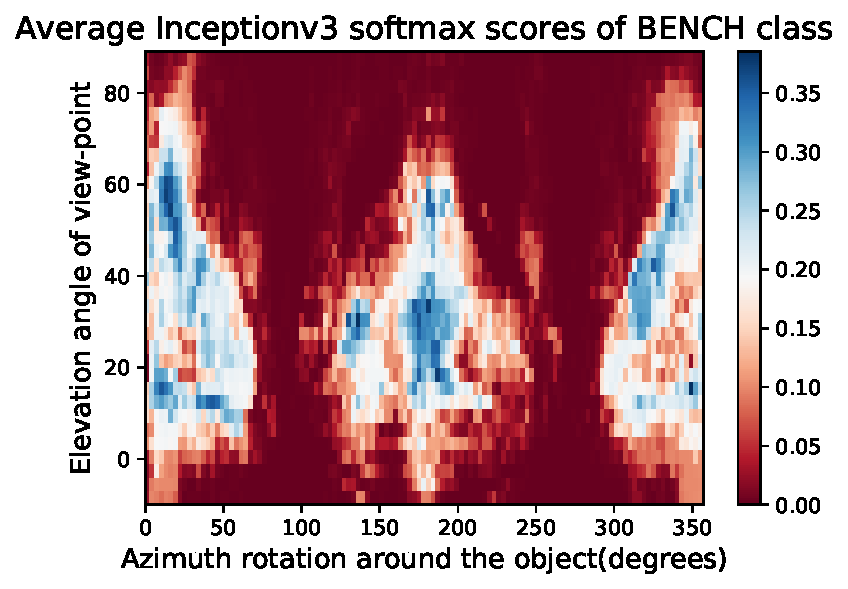
\includegraphics[width = 4cm]{supimages/nms2d/Inceptionv3_bench_Average.pdf}\\ \hline
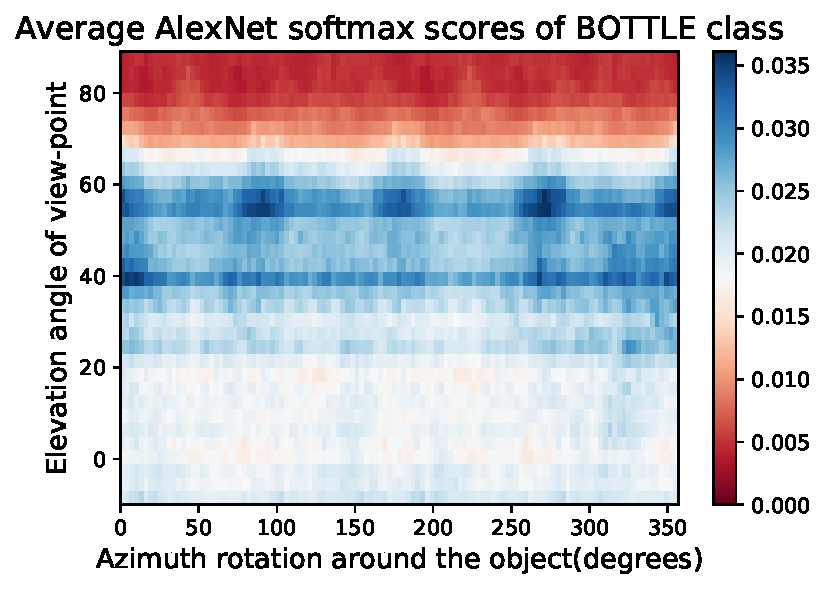
\includegraphics[width = 4cm]{supimages/nms2d/AlexNet_bottle_Average.pdf}&
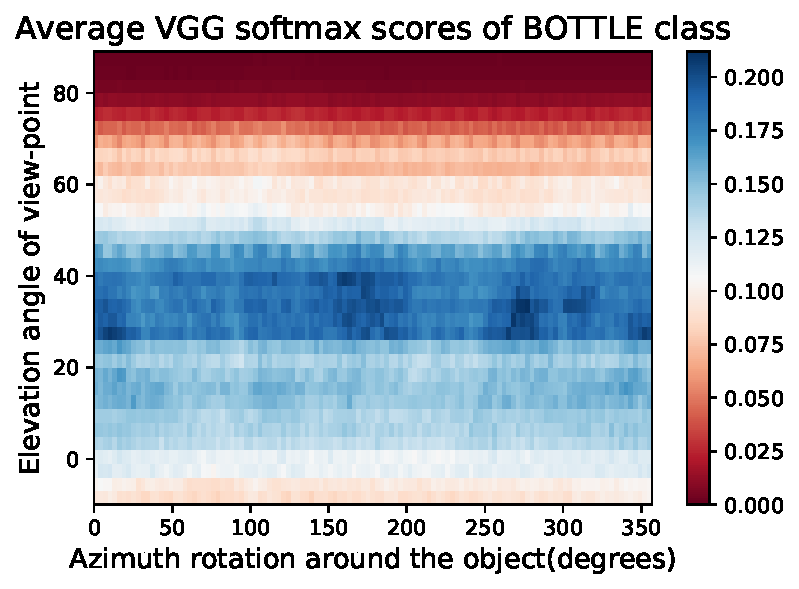
\includegraphics[width = 4cm]{supimages/nms2d/VGG_bottle_Average.pdf}&
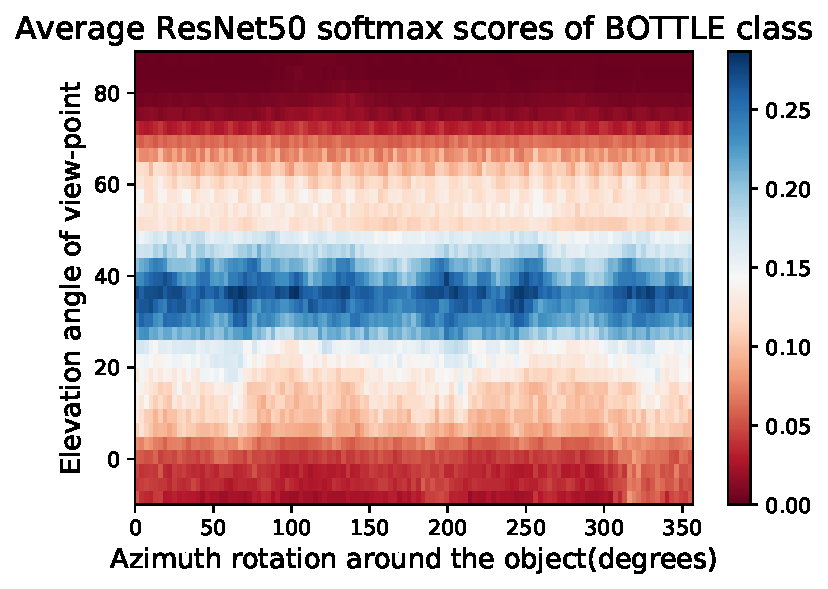
\includegraphics[width = 4cm]{supimages/nms2d/ResNet50_bottle_Average.pdf}&
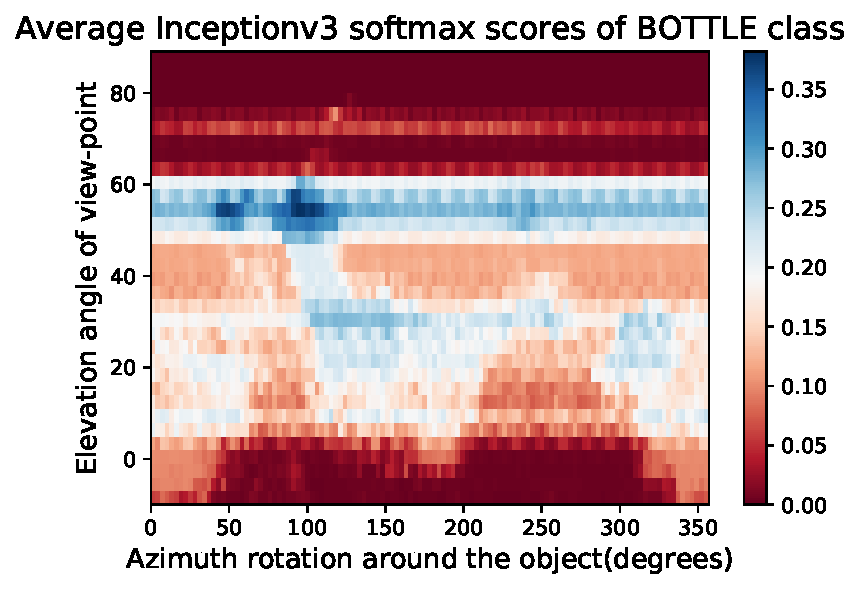
\includegraphics[width = 4cm]{supimages/nms2d/Inceptionv3_bottle_Average.pdf} \\\hline
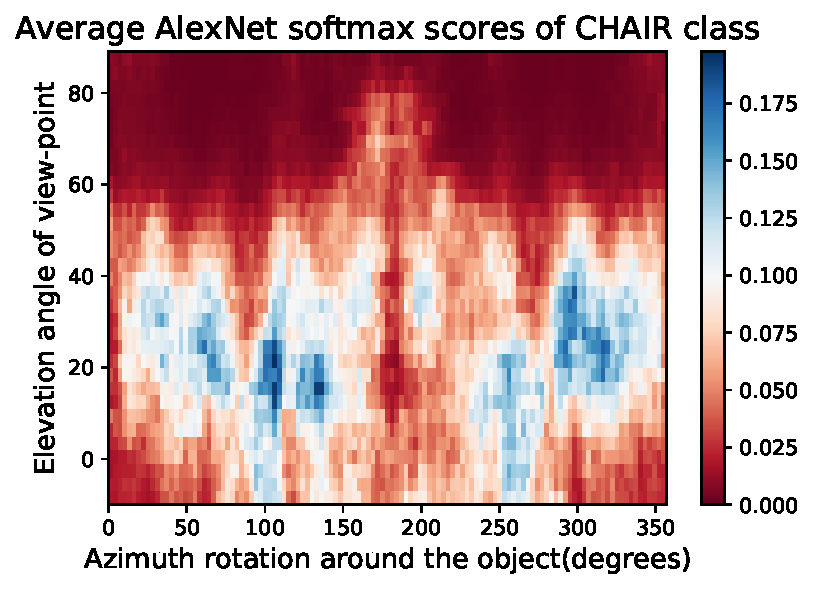
\includegraphics[width = 4cm]{supimages/nms2d/AlexNet_chair_Average.pdf}&
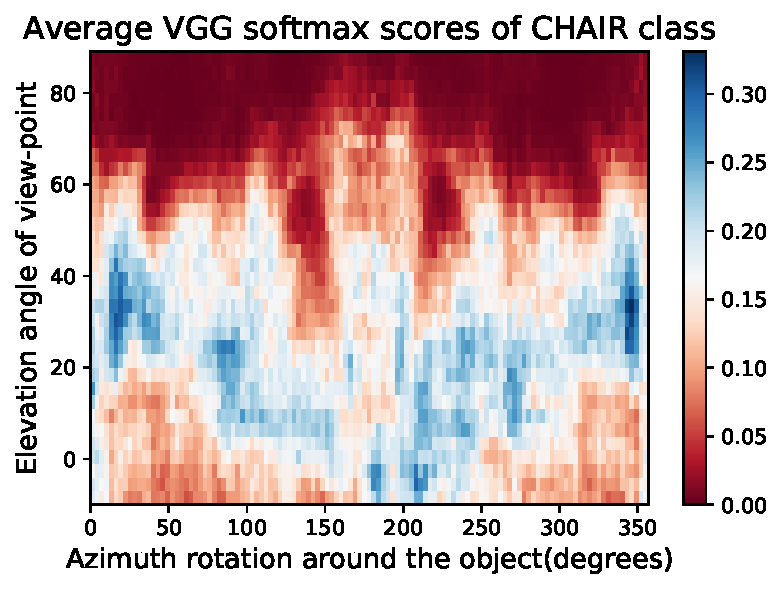
\includegraphics[width = 4cm]{supimages/nms2d/VGG_chair_Average.pdf}&
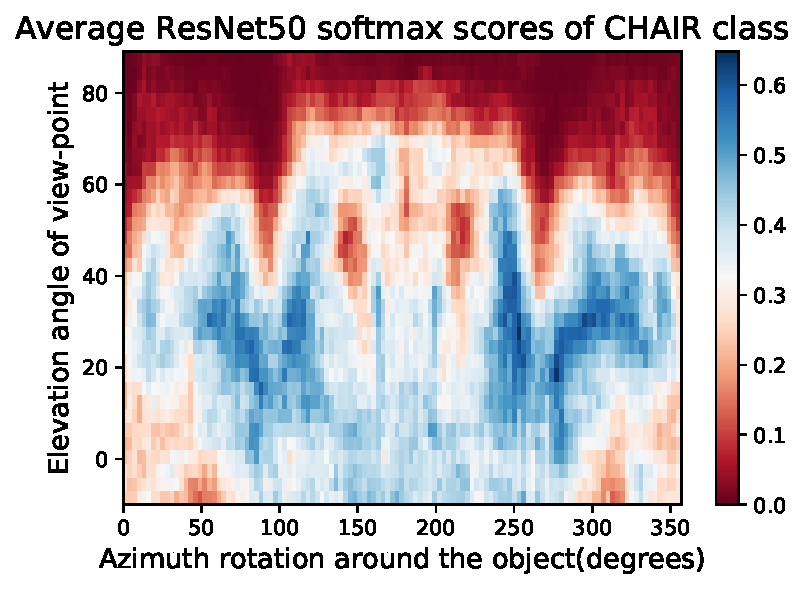
\includegraphics[width = 4cm]{supimages/nms2d/ResNet50_chair_Average.pdf}&
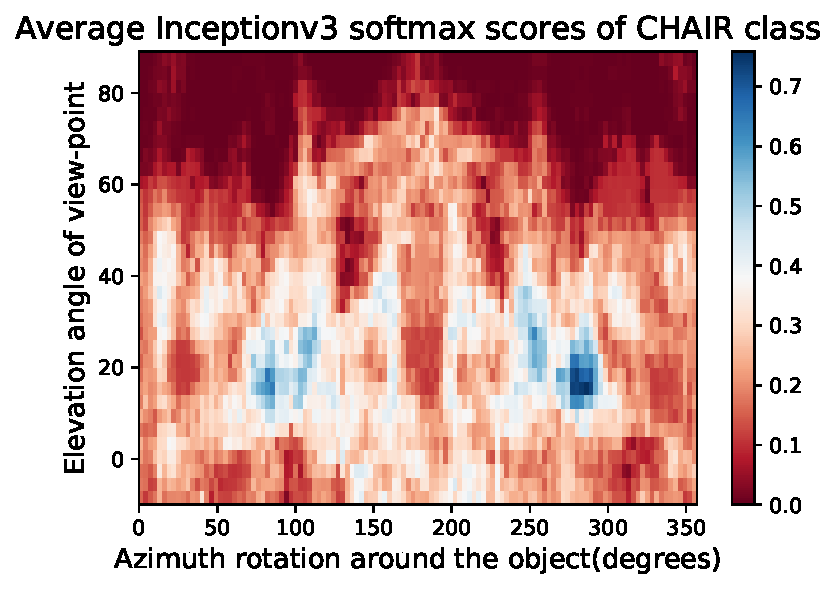
\includegraphics[width = 4cm]{supimages/nms2d/Inceptionv3_chair_Average.pdf} \\
% 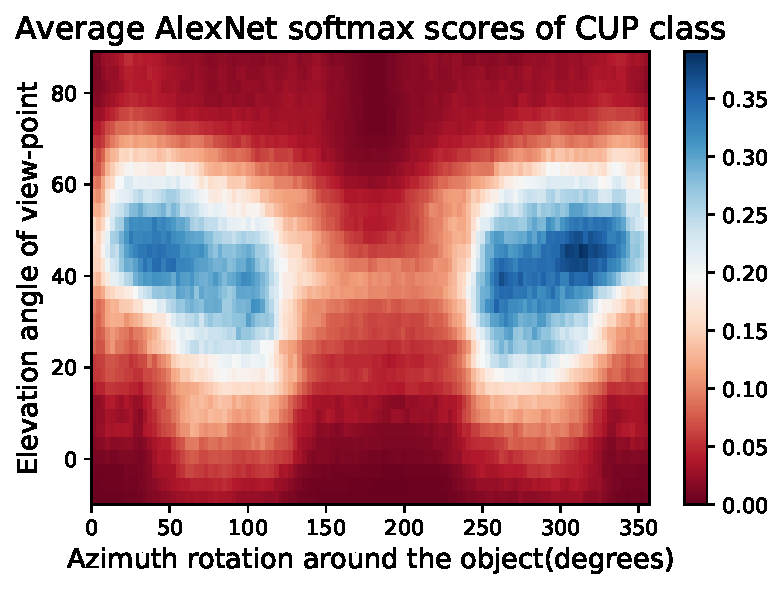
\includegraphics[width = 4cm]{supimages/nms2d/AlexNet_cup_Average.pdf}&
% 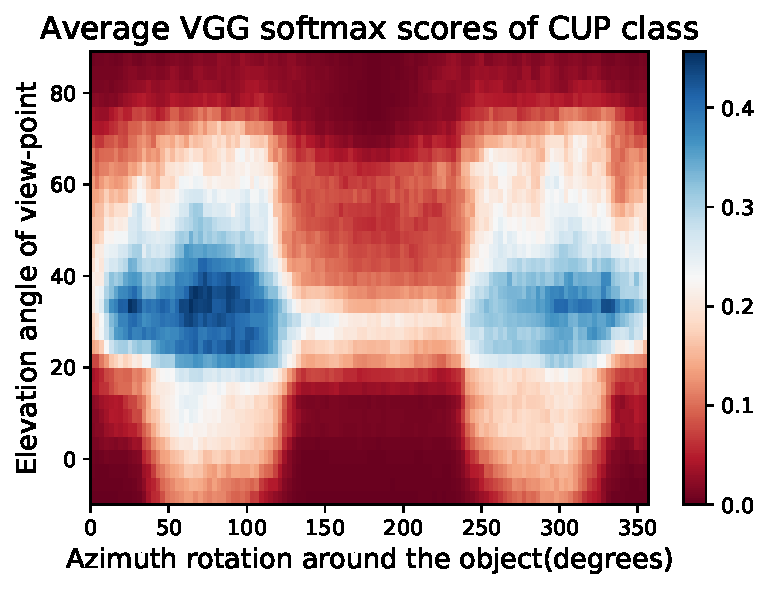
\includegraphics[width = 4cm]{supimages/nms2d/VGG_cup_Average.pdf}&
% 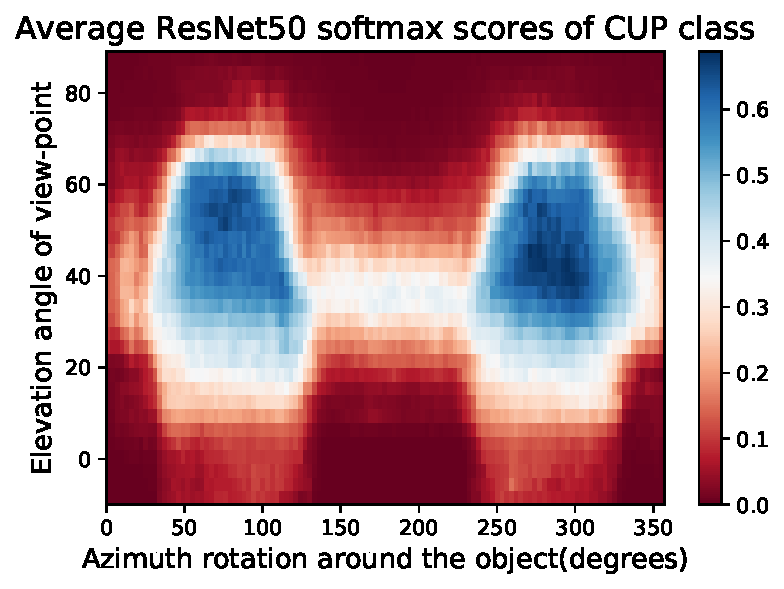
\includegraphics[width = 4cm]{supimages/nms2d/ResNet50_cup_Average.pdf}&
% 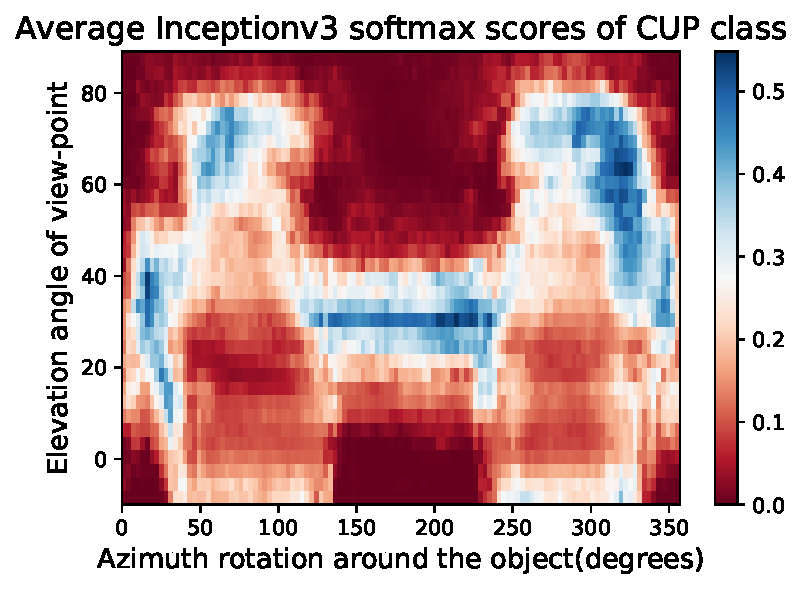
\includegraphics[width = 4cm]{supimages/nms2d/Inceptionv3_cup_Average.pdf}\\ 
% 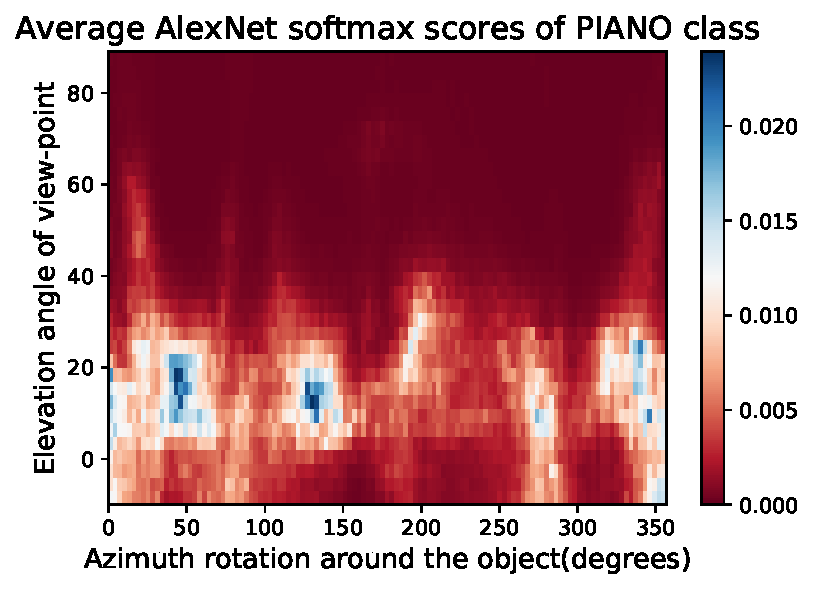
\includegraphics[width = 4cm]{supimages/nms2d/AlexNet_piano_Average.pdf}&
% 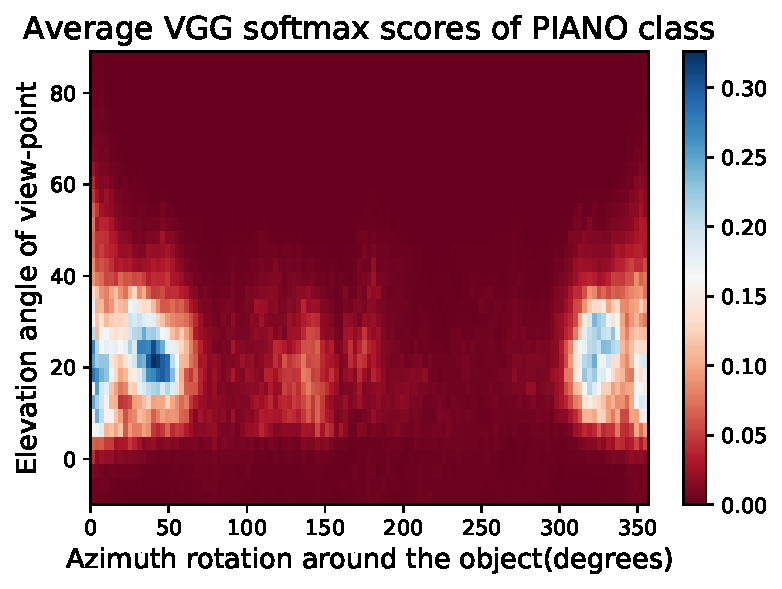
\includegraphics[width = 4cm]{supimages/nms2d/VGG_piano_Average.pdf}&
% 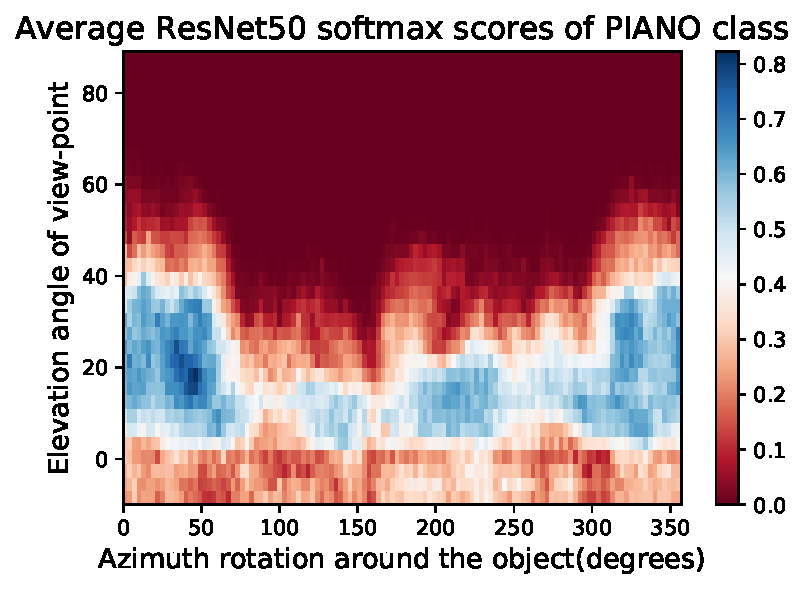
\includegraphics[width = 4cm]{supimages/nms2d/ResNet50_piano_Average.pdf}&
% 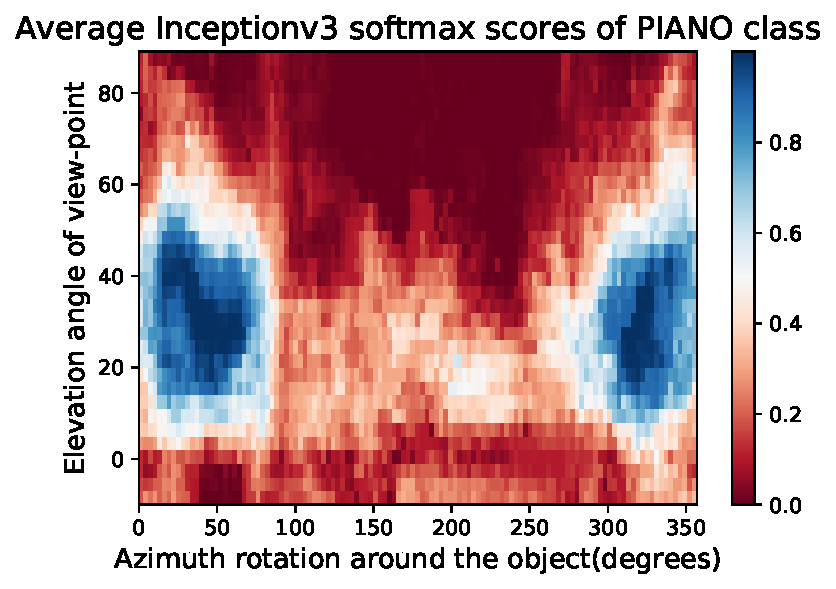
\includegraphics[width = 4cm]{supimages/nms2d/Inceptionv3_piano_Average.pdf}\\ 
% 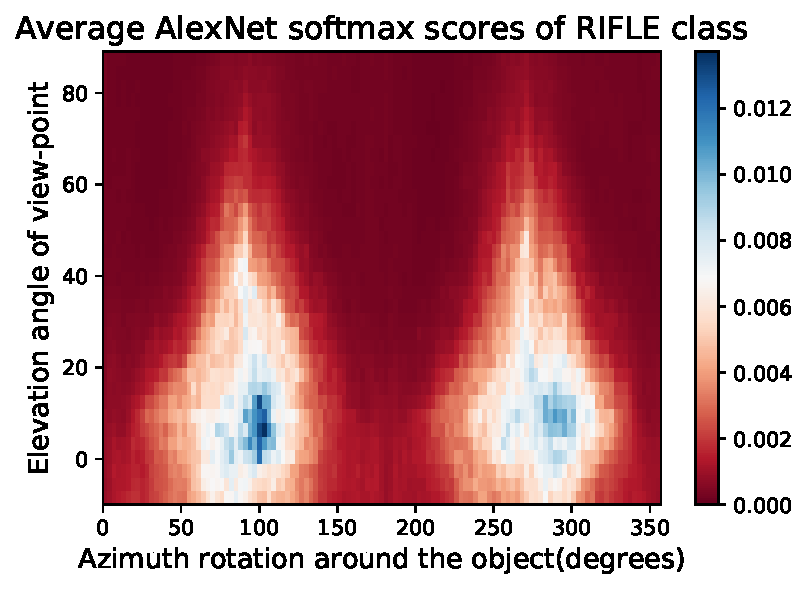
\includegraphics[width = 4cm]{supimages/nms2d/AlexNet_rifle_Average.pdf}&
% 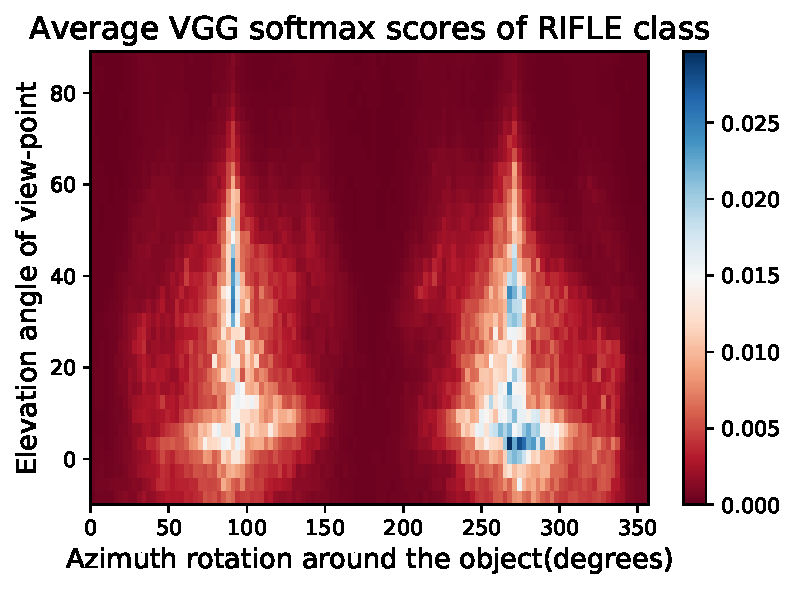
\includegraphics[width = 4cm]{supimages/nms2d/VGG_rifle_Average.pdf}&
% \includegraphics[width = 4cm]{supimages/nms2d/ResNet50_rifle_Average.pdf}&
% \includegraphics[width = 4cm]{supimages/nms2d/Inceptionv3_rifle_Average.pdf}\\ 
% \includegraphics[width = 4cm]{supimages/nms2d/AlexNet_vase_Average.pdf}&
% \includegraphics[width = 4cm]{supimages/nms2d/VGG_vase_Average.pdf}&
% \includegraphics[width = 4cm]{supimages/nms2d/ResNet50_vase_Average.pdf}&
% \includegraphics[width = 4cm]{supimages/nms2d/Inceptionv3_vase_Average.pdf}\\ 
% \includegraphics[width = 4cm]{supimages/nms2d/AlexNet_toilet_Average.pdf}&
% \includegraphics[width = 4cm]{supimages/nms2d/VGG_toilet_Average.pdf}&
% \includegraphics[width = 4cm]{supimages/nms2d/ResNet50_toilet_Average.pdf}&
% \includegraphics[width = 4cm]{supimages/nms2d/Inceptionv3_toilet_Average.pdf}
\hline
\end{tabular}
    %   \vspace{-9pt}
   \caption{\small \textbf{2D Network Semantic Maps NMS-I}. Visualizing 2D Semantic Robustness profile for different networks averaged over 10 different shapes. Every row is different class. observe that different DNNs profiles differ depending on the training , accuracy , and network architectures that all result in a unique ''signatures" for the DNN on that class.}
   \vspace{-8pt}
   \label{fig:nsm2d-1}
\end{figure*}

\begin{figure*}[h]
\centering
\tabcolsep=0.03cm
   \begin{tabular}{||c|c|c|c||} \hline
   \textbf{AlexNet} & \textbf{VGG} &\textbf{ResNet50} & \textbf{InceptionV3} \\ \hline
% \includegraphics[width = 4cm]{supimages/nms2d/AlexNet_aeroplane_Average.pdf}&
% \includegraphics[width = 4cm]{supimages/nms2d/VGG_aeroplane_Average.pdf}&
% \includegraphics[width = 4cm]{supimages/nms2d/ResNet50_aeroplane_Average.pdf}&
% \includegraphics[width = 4cm]{supimages/nms2d/Inceptionv3_aeroplane_Average.pdf}\\ 
% \includegraphics[width = 4cm]{supimages/nms2d/AlexNet_bathtub_Average.pdf}&
% \includegraphics[width = 4cm]{supimages/nms2d/VGG_bathtub_Average.pdf}&
% \includegraphics[width = 4cm]{supimages/nms2d/ResNet50_bathtub_Average.pdf}&
% \includegraphics[width = 4cm]{supimages/nms2d/Inceptionv3_bathtub_Average.pdf}\\ 
% \includegraphics[width = 4cm]{supimages/nms2d/AlexNet_bench_Average.pdf}&
% \includegraphics[width = 4cm]{supimages/nms2d/VGG_bench_Average.pdf}&
% \includegraphics[width = 4cm]{supimages/nms2d/ResNet50_bench_Average.pdf}&
% \includegraphics[width = 4cm]{supimages/nms2d/Inceptionv3_bench_Average.pdf}\\ 
% \includegraphics[width = 4cm]{supimages/nms2d/AlexNet_bottle_Average.pdf}&
% \includegraphics[width = 4cm]{supimages/nms2d/VGG_bottle_Average.pdf}&
% \includegraphics[width = 4cm]{supimages/nms2d/ResNet50_bottle_Average.pdf}&
% \includegraphics[width = 4cm]{supimages/nms2d/Inceptionv3_bottle_Average.pdf}\\ 
% \includegraphics[width = 4cm]{supimages/nms2d/AlexNet_chair_Average.pdf}&
% \includegraphics[width = 4cm]{supimages/nms2d/VGG_chair_Average.pdf}&
% \includegraphics[width = 4cm]{supimages/nms2d/ResNet50_chair_Average.pdf}&
% \includegraphics[width = 4cm]{supimages/nms2d/Inceptionv3_chair_Average.pdf}\\ 
\includegraphics[width = 4cm]{supimages/nms2d/AlexNet_cup_Average.pdf}&
\includegraphics[width = 4cm]{supimages/nms2d/VGG_cup_Average.pdf}&
\includegraphics[width = 4cm]{supimages/nms2d/ResNet50_cup_Average.pdf}&
\includegraphics[width = 4cm]{supimages/nms2d/Inceptionv3_cup_Average.pdf}\\ \hline
\includegraphics[width = 4cm]{supimages/nms2d/AlexNet_piano_Average.pdf}&
\includegraphics[width = 4cm]{supimages/nms2d/VGG_piano_Average.pdf}&
\includegraphics[width = 4cm]{supimages/nms2d/ResNet50_piano_Average.pdf}&
\includegraphics[width = 4cm]{supimages/nms2d/Inceptionv3_piano_Average.pdf}\\ \hline
\includegraphics[width = 4cm]{supimages/nms2d/AlexNet_rifle_Average.pdf}&
\includegraphics[width = 4cm]{supimages/nms2d/VGG_rifle_Average.pdf}&
\includegraphics[width = 4cm]{supimages/nms2d/ResNet50_rifle_Average.pdf}&
\includegraphics[width = 4cm]{supimages/nms2d/Inceptionv3_rifle_Average.pdf}\\ \hline
\includegraphics[width = 4cm]{supimages/nms2d/AlexNet_vase_Average.pdf}&
\includegraphics[width = 4cm]{supimages/nms2d/VGG_vase_Average.pdf}&
\includegraphics[width = 4cm]{supimages/nms2d/ResNet50_vase_Average.pdf}&
\includegraphics[width = 4cm]{supimages/nms2d/Inceptionv3_vase_Average.pdf}\\ \hline
\includegraphics[width = 4cm]{supimages/nms2d/AlexNet_toilet_Average.pdf}&
\includegraphics[width = 4cm]{supimages/nms2d/VGG_toilet_Average.pdf}&
\includegraphics[width = 4cm]{supimages/nms2d/ResNet50_toilet_Average.pdf}&
\includegraphics[width = 4cm]{supimages/nms2d/Inceptionv3_toilet_Average.pdf} \\
\hline
\end{tabular}
    %   \vspace{-9pt}
   \caption{\small \textbf{2D Network Semantic Maps NMS-II}: visualizing 2D Semantic Robustness profile for different networks averaged over 10 different shapes. Every row is different class. observe that different DNNs profiles differ depending on the training , accuracy , and network architectures that all result in a unique ''signatures" for the DNN on that class.}
   \vspace{-8pt}
   \label{fig:nsm2d-2}
\end{figure*}


% \clearpage

% \clearpage
%%%%%%%%%%%%%%%%%%%%%%%%%%%%%%%%%%%%%%%%
\subsection{Convergence of the Region Finding Algorithms}
Here we show how when we apply the region detection algorithms; the naive detect the smallest region while the OIR formulations detect bigger more general robust region. This result happens even with different initial points; they always converge to the same bounds of that robust region of the semantic maps. \figLabel{\ref{fig:converge}} show 4 different initializations for 1D case  along with predicted regions. In \figLabel{\ref{fig:conv1},\ref{fig:conv2}} shows the bounds evolving during the optimization of the three algorithms (naive , OIR\_B and OIR\_W ) for 500 steps.
\begin{figure*}[h]
\centering
\tabcolsep=0.03cm
\includegraphics[width = \textwidth]{supimages/converge/1D_bathtub_regions.pdf}
   \caption{\small \textbf{Robust Region Detection with different initializations}: visualizing the Robust Regions Bounds found by the three algorithms for four initial points. We can see that the naive produce different bounds of the same region for different initializations while OIR detect the same region regardless of initialization.}
   \vspace{-8pt}
   \label{fig:converge}
\end{figure*}
\begin{figure*}[h]
\centering
\tabcolsep=0.03cm
   \begin{tabular}{c|c}  \hline
   \textbf{initialization = 120} & \textbf{initialization = 140} \\  \hline 
   \multicolumn{2}{c}{\textbf{Naive algorithm}} \\   
\includegraphics[width = 9cm]{supimages/converge/run0_1_1_naive.pdf} &
\includegraphics[width = 9cm]{supimages/converge/run1_1_1_naive.pdf} \\   \hline
\multicolumn{2}{c}{\textbf{Black-Box OIR algorithm}} \\  
\includegraphics[width = 9cm]{supimages/converge/run0_1_1_OIR_B.pdf} &
\includegraphics[width = 9cm]{supimages/converge/run1_1_1_OIR_B.pdf} \\   \hline
\multicolumn{2}{c}{\textbf{White-Box OIR algorithm}} \\  
\includegraphics[width = 9cm]{supimages/converge/run0_1_1_OIR_W.pdf} &
\includegraphics[width = 9cm]{supimages/converge/run1_1_1_OIR_W.pdf} \\   \hline
\end{tabular}
    %   \vspace{-9pt}
   \caption{\small \textbf{Robust Region Bounds Growing I}: visualizing the bounds growing Using different algorithms from two different initializations (120 and 140) in \figLabel{\ref{fig:converge}}. We can see that OIR formulations converge to the same bounds of the robust region regardless of the initialization, which indicates effectiveness in detecting these regions, unlike the naive approach which can stop in a local optimum. }
   \vspace{-8pt}
   \label{fig:conv1}
\end{figure*}

\begin{figure*}[h]
\centering
\tabcolsep=0.03cm
   \begin{tabular}{c|c}  \hline
   \textbf{initialization = 290} & \textbf{initialization = 310} \\  \hline
      \multicolumn{2}{c}{\textbf{Naive algorithm}} \\   
\includegraphics[width = 9cm]{supimages/converge/run2_1_1_naive.pdf} &
\includegraphics[width = 9cm]{supimages/converge/run3_1_1_naive.pdf} \\   \hline
\multicolumn{2}{c}{\textbf{Black-Box OIR algorithm}} \\  
\includegraphics[width = 9cm]{supimages/converge/run2_1_1_OIR_B.pdf} &
\includegraphics[width = 9cm]{supimages/converge/run3_1_1_OIR_B.pdf} \\   \hline
\multicolumn{2}{c}{\textbf{White-Box OIR algorithm}} \\ 
\includegraphics[width = 9cm]{supimages/converge/run2_1_1_OIR_W.pdf} &
\includegraphics[width = 9cm]{supimages/converge/run3_1_1_OIR_W.pdf} \\   \hline
\end{tabular}
    %   \vspace{-9pt}
   \caption{\small \textbf{Robust Region Bounds Growing I}: visualizing the bounds growing Using different algorithms from two different initializations (290, 310) in \figLabel{\ref{fig:converge}}. We can see that OIR formulations converge to the same bounds of the robust region regardless of the initialization, which indicates effectiveness in detecting these regions, unlike the naive approach which can stop in a local optimum. }
   \vspace{-8pt}
   \label{fig:conv2}
\end{figure*}


% \clearpage
%%%%%%%%%%%%%%%%%%%%%%%%%%%%%%%%%%%%%%%%
\subsection{Examples of Found Regions ( with Example Renderings)}
In \figLabel{\ref{fig:ex1},\ref{fig:ex2}} we provide examples of 2D regions found with the three algorithms along with renderings of the shapes from the robust regions detected.

% \begin{figure*}[h]
% \centering
% \tabcolsep=0.03cm
%   \begin{tabular}[!t]{c|c}  \hline
%   \textbf{Detected Robust Regions} & \textbf{Renderings from Inside the Regions} \\  \hline
% \includegraphics[width = 8.5cm]{supimages/qualitative/AlexNet_chair_6_regions.pdf} &
% \begin{tabular}[t]{ccc} 
%  \includegraphics[width = 2cm]{supimages/qualitative/chair/20_110.jpg} &\includegraphics[width = 2cm]{supimages/qualitative/chair/20_130.jpg} &\includegraphics[width = 2cm]{supimages/qualitative/chair/40_120.jpg}
%  \end{tabular}\\ \hline 
% \includegraphics[width = 8.5cm]{supimages/qualitative/Inceptionv3_aeroplane_7_regions.pdf} & 
% \begin{tabular}[t]{ccc} 
%  \includegraphics[width = 2cm]{supimages/qualitative/aeroplane/10_40.jpg} &\includegraphics[width = 2cm]{supimages/qualitative/aeroplane/30_50.jpg} &\includegraphics[width = 2cm]{supimages/qualitative/aeroplane/10_60.jpg}
%  \end{tabular}\\ \hline 
% \includegraphics[width = 8.5cm]{supimages/qualitative/Inceptionv3_bench_0_regions.pdf} & \begin{tabular}[t]{ccc} 
%  \includegraphics[width = 2cm]{supimages/qualitative/bench/0_10.jpg} &\includegraphics[width = 2cm]{supimages/qualitative/bench/20_50.jpg} &\includegraphics[width = 2cm]{supimages/qualitative/bench/50_50.jpg}
%  \end{tabular}\\ \hline 
% \includegraphics[width = 8.5cm]{supimages/qualitative/Inceptionv3_bottle_2_regions.pdf} & \begin{tabular}[t]{ccc} 
%  \includegraphics[width = 2cm]{supimages/qualitative/bottle/0_180.jpg} &\includegraphics[width = 2cm]{supimages/qualitative/bottle/10_210.jpg} &\includegraphics[width = 2cm]{supimages/qualitative/bottle/30_180.jpg}
%  \end{tabular}\\ \hline 
% % \includegraphics[width = 8.5cm]{supimages/qualitative/Inceptionv3_cup_1_regions.pdf} & \\ \hline 
% % \includegraphics[width = 8.5cm]{supimages/qualitative/Inceptionv3_piano_1_regions.pdf} & \\ \hline 
% % \includegraphics[width = 8.5cm]{supimages/qualitative/Inceptionv3_toilet_0_regions.pdf} & \\ \hline 
% % \includegraphics[width = 8.5cm]{supimages/qualitative/ResNet50_rifle_1_regions.pdf} & \\ \hline 
% % \includegraphics[width = 8.5cm]{supimages/qualitative/VGG_bathtub_4_regions.pdf} & \\ \hline 
% \end{tabular}
%     %   \vspace{-9pt}
%   \caption{\small \textbf{Qualitative Examples of Robust Regions I}: visualizing different runs of the algorithm to find robust regions along with different renderings from inside these regions for those specific shapes used in the experiments. }
%   \vspace{-8pt}
%   \label{fig:ex1}
% \end{figure*}
\begin{figure*}[h]
\centering
\tabcolsep=0.03cm
   \begin{tabular}[!t]{c|c}  \hline
   \textbf{Detected Robust Regions} & \textbf{Renderings from Inside the Robust Regions} \\  \hline
\includegraphics[width = 8.5cm]{supimages/qualitative/AlexNet_chair_6_regions.pdf} &
 \includegraphics[width = 7.5cm]{supimages/qualitative/chair/chair_s.png}\\ \hline 
 \includegraphics[width = 9.5cm]{supimages/qualitative/Inceptionv3_aeroplane_7_regions.pdf} & 
 \includegraphics[width = 7.5cm]{supimages/qualitative/aeroplane/aeroplane_s.png}\\ \hline 
\includegraphics[width = 9.5cm]{supimages/qualitative/Inceptionv3_bench_0_regions.pdf} & 
 \includegraphics[width = 7.5cm]{supimages/qualitative/bench/bench_s.png}\\ \hline 
\includegraphics[width = 9.5cm]{supimages/qualitative/Inceptionv3_bottle_2_regions.pdf}  &
 \includegraphics[width = 7.5cm]{supimages/qualitative/bottle/bottle_s.png}\\ \hline 
% \includegraphics[width = 8.5cm]{supimages/qualitative/Inceptionv3_cup_1_regions.pdf} & \\ \hline 
% \includegraphics[width = 8.5cm]{supimages/qualitative/Inceptionv3_piano_1_regions.pdf} & \\ \hline 
% \includegraphics[width = 8.5cm]{supimages/qualitative/Inceptionv3_toilet_0_regions.pdf} & \\ \hline 
% \includegraphics[width = 8.5cm]{supimages/qualitative/ResNet50_rifle_1_regions.pdf} & \\ \hline 
% \includegraphics[width = 8.5cm]{supimages/qualitative/VGG_bathtub_4_regions.pdf} & \\ \hline 
\end{tabular}
    %   \vspace{-9pt}
   \caption{\small \textbf{Qualitative Examples of Robust Regions I}: visualizing different runs of the algorithm to find robust regions along with different renderings from inside these regions for those specific shapes used in the experiments. }
  \vspace{-8pt}
   \label{fig:ex1}
\end{figure*}

% \begin{figure*}[h]
% \centering
% \tabcolsep=0.03cm
%   \begin{tabular}{c|c}  \hline
%   \textbf{Detected Robust Regions} & \textbf{Renderings from Inside the Regions} \\  \hline
% % \includegraphics[width = 8.5cm]{supimages/qualitative/AlexNet_chair_6_regions.pdf} & \\ \hline 
% % \includegraphics[width = 8.5cm]{supimages/qualitative/Inceptionv3_aeroplane_7_regions.pdf} & \\ \hline 
% % % \includegraphics[width = 8.5cm]{supimages/qualitative/Inceptionv3_bench_0_regions.pdf} & \\ \hline 
% % \includegraphics[width = 8.5cm]{supimages/qualitative/Inceptionv3_bottle_2_regions.pdf} & 
% % \begin{tabular}[t]{ccc} 
% %  \includegraphics[width = 2cm]{supimages/qualitative/chair/20_110.jpg} &\includegraphics[width = 2cm]{supimages/qualitative/chair/20_110.jpg} &\includegraphics[width = 2cm]{supimages/qualitative/chair/20_110.jpg}
% %  \end{tabular}\\ \hline 
% \includegraphics[width = 8.5cm]{supimages/qualitative/Inceptionv3_cup_1_regions.pdf} & 
% \begin{tabular}[t]{ccc} 
%  \includegraphics[width = 2cm]{supimages/qualitative/cup/30_280.jpg} &\includegraphics[width = 2cm]{supimages/qualitative/cup/40_320.jpg} &\includegraphics[width = 2cm]{supimages/qualitative/cup/60_290.jpg}
%  \end{tabular}\\ \hline 
% \includegraphics[width = 8.5cm]{supimages/qualitative/Inceptionv3_piano_1_regions.pdf} & 
% \begin{tabular}[t]{ccc} 
%  \includegraphics[width = 2cm]{supimages/qualitative/piano/10_0.jpg} &\includegraphics[width = 2cm]{supimages/qualitative/piano/30_50.jpg} &\includegraphics[width = 2cm]{supimages/qualitative/piano/60_10.jpg}
%  \end{tabular}\\ \hline 
%  \includegraphics[width = 8.5cm]{supimages/qualitative/ResNet50_rifle_1_regions.pdf} & 
% \begin{tabular}[t]{ccc} 
%  \includegraphics[width = 2cm]{supimages/qualitative/rifle/10_50.jpg} &\includegraphics[width = 2cm]{supimages/qualitative/rifle/20_120.jpg} &\includegraphics[width = 2cm]{supimages/qualitative/rifle/50_80.jpg}
%  \end{tabular}\\ \hline 
% % \includegraphics[width = 8.5cm]{supimages/qualitative/Inceptionv3_toilet_0_regions.pdf} & \\ \hline 
% % \includegraphics[width = 8.5cm]{supimages/qualitative/ResNet50_rifle_1_regions.pdf} & \\ \hline 
% % \includegraphics[width = 8.5cm]{supimages/qualitative/VGG_bathtub_4_regions.pdf} & \\ \hline 
% \end{tabular}
%     %   \vspace{-9pt}
%   \caption{\small \textbf{Qualitative Examples of Robust Regions II}: visualizing different runs of the algorithm to find robust regions along with different renderings from inside these regions for those specific shapes used in the experiments.}
%   \vspace{-8pt}
%   \label{fig:ex2}
% \end{figure*}
\begin{figure*}[h]
\centering
\tabcolsep=0.03cm
   \begin{tabular}{c|c}  \hline
   \textbf{Detected Robust Regions} & \textbf{Renderings from Inside the Robust Regions} \\  \hline
% \includegraphics[width = 8.5cm]{supimages/qualitative/AlexNet_chair_6_regions.pdf} & \\ \hline 
% \includegraphics[width = 8.5cm]{supimages/qualitative/Inceptionv3_aeroplane_7_regions.pdf} & \\ \hline 
% % \includegraphics[width = 8.5cm]{supimages/qualitative/Inceptionv3_bench_0_regions.pdf} & \\ \hline 
% \includegraphics[width = 8.5cm]{supimages/qualitative/Inceptionv3_bottle_2_regions.pdf} & 
% \begin{tabular}[t]{ccc} 
%  \includegraphics[width = 2cm]{supimages/qualitative/chair/20_110.jpg} &\includegraphics[width = 2cm]{supimages/qualitative/chair/20_110.jpg} &\includegraphics[width = 2cm]{supimages/qualitative/chair/20_110.jpg}
%  \end{tabular}\\ \hline 
\includegraphics[width = 9.5cm]{supimages/qualitative/Inceptionv3_cup_1_regions.pdf} & 
 \includegraphics[width = 7.5cm]{supimages/qualitative/cup/cup_s.png}\\ \hline 
\includegraphics[width = 9.5cm]{supimages/qualitative/Inceptionv3_piano_1_regions.pdf} &  
\includegraphics[width = 7.5cm]{supimages/qualitative/piano/piano_s.png}\\ \hline 
 \includegraphics[width = 9.5cm]{supimages/qualitative/ResNet50_rifle_1_regions.pdf} & 
  \includegraphics[width = 7.5cm]{supimages/qualitative/rifle/rifle_s.png}\\ \hline 
% \includegraphics[width = 8.5cm]{supimages/qualitative/Inceptionv3_toilet_0_regions.pdf} & \\ \hline 
% \includegraphics[width = 8.5cm]{supimages/qualitative/ResNet50_rifle_1_regions.pdf} & \\ \hline 
% \includegraphics[width = 8.5cm]{supimages/qualitative/VGG_bathtub_4_regions.pdf} & \\ \hline 
\end{tabular}
    %   \vspace{-9pt}
   \caption{\small \textbf{Qualitative Examples of Robust Regions II}: visualizing different runs of the algorithm to find robust regions along with different renderings from inside these regions for those specific shapes used in the experiments.}
   \vspace{-8pt}
   \label{fig:ex2}
\end{figure*}



% \clearpage
%%%%%%%%%%%%%%%%%%%%%%%%%%%%%%%%%%%%%%%%%%%%%%%%%%%%%%%%%%%%%%
\subsection{Analyzing Semantic Data Bias in ImageNet}
In \figLabel{\ref{fig:dsm1},\ref{fig:dsm2}}, we visualizing semantic data bias in the common training dataset (\ie ImageNet \cite{IMAGENET}) by averaging the Networks Semantic Maps (NSM) of different networks and on different shapes, Different classes have a different semantic bias in ImageNet as clearly shown in the maps above. These places of high confidence probably reveal the areas where an abundance of examples exists in ImageNet, while holes convey scarcity of such examples in ImageNet corresponding class.
\begin{figure*}[h]
\centering
\tabcolsep=0.03cm
   \begin{tabular}{c|c}
\includegraphics[width = 9cm]{supimages/bias/aeroplane_Average_2D.pdf}&
\includegraphics[width = 9cm]{supimages/bias/bathtub_Average_2D.pdf}\\\hline
\includegraphics[width = 9cm]{supimages/bias/bench_Average_2D.pdf}&
\includegraphics[width = 9cm]{supimages/bias/bottle_Average_2D.pdf}
% \includegraphics[width = 9cm]{supimages/bias/chair_Average_2D.pdf}&
% \includegraphics[width = 9cm]{supimages/bias/cup_Average_2D.pdf}\\
% \includegraphics[width = 9cm]{supimages/bias/piano_Average_2D.pdf}&
% \includegraphics[width = 9cm]{supimages/bias/rifle_Average_2D.pdf}\\
% \includegraphics[width = 9cm]{supimages/bias/vase_Average_2D.pdf}&
% \includegraphics[width = 9cm]{supimages/bias/toilet_Average_2D.pdf}
\end{tabular}
    %   \vspace{-9pt}
   \caption{\small \textbf{Data Semantic Maps DSM-I}: visualizing Semantic Data Bias in the common training dataset (\ie ImageNet \cite{IMAGENET}) by averaging the Networks Semantic Maps (NSM) of different networks and on different shapes, Different classes have different semantic bias in ImageNet as clearly shown in the maps above. The symmetry in the maps are attributed to the 3D symmetry of the objects. }
   \vspace{-8pt}
   \label{fig:dsm1}
\end{figure*}

\begin{figure*}[]
\centering
\tabcolsep=0.03cm
   \begin{tabular}{c|c}
% \includegraphics[width = 9cm]{supimages/bias/aeroplane_Average_2D.pdf}&
% \includegraphics[width = 9cm]{supimages/bias/bathtub_Average_2D.pdf}\\
% \includegraphics[width = 9cm]{supimages/bias/bench_Average_2D.pdf}&
% \includegraphics[width = 9cm]{supimages/bias/bottle_Average_2D.pdf}\\
\includegraphics[width = 9cm]{supimages/bias/chair_Average_2D.pdf}&
\includegraphics[width = 9cm]{supimages/bias/cup_Average_2D.pdf}\\\hline
\includegraphics[width = 9cm]{supimages/bias/piano_Average_2D.pdf}&
\includegraphics[width = 9cm]{supimages/bias/rifle_Average_2D.pdf}\\\hline
\includegraphics[width = 9cm]{supimages/bias/vase_Average_2D.pdf}&
\includegraphics[width = 9cm]{supimages/bias/toilet_Average_2D.pdf}
\end{tabular}
    %   \vspace{-9pt}
   \caption{\small \textbf{Data Semantic Maps DSM-II}: visualizing Semantic Data Bias in the common training dataset (\ie ImageNet \cite{IMAGENET}) By averaging the Networks Semantic Maps (NSM) of different networks and on different shapes, Different classes have different semantic bias in ImageNet as clearly shown in the maps above. The symmetry in the maps are attributed to the 3D symmetry of the objects.}
   \vspace{-8pt}
   \label{fig:dsm2}
\end{figure*}


\clearpage
%%%%%%%%%%%%%%%%%%%%%%%%%%%%%%%%%%%%%%%%
\section{Detailed Derivations of the Update Directions of the Bounds}
% \M{Show all the derivations as well as the unised formulations }
% Typical adversarial pixel attacks involve a neural network agent $\mathbf{C}$ (\eg classifier or detector) that takes an image $\mathbf{x} \in [0,1]^{d}$ as input and outputs a multinoulli distribution over $K$ class labels with softmax values $[l_{1}, l_{2}, ... ,l_{K}]$, where $l_{j}$ is the softmax value for class $j$. The adversary (attacker) tries to produce a perturbed image $\mathbf{x'} \in [0,1]^{d}$ that is as close as possible to $\mathbf{x}$ and where $\mathbf{C}(\mathbf{x}) \ne \mathbf{C}(\mathbf{x'})$. %while maintaining a small distance $\mathit{d}(\mathbf{x},\mathbf{x'})< \epsilon$. 
% The objective to be optimized can be formulated as follows: 
% \begin{equation}
% \begin{aligned} 
%  &\min_{\mathbf{x'}} ~ \mathit{d}(\mathbf{x},\mathbf{x'})~~~ \text{s.t.~}  \mathbf{C}(\mathbf{x}) \ne \mathbf{C}(\mathbf{x'});~ \mathbf{x'} \in [0,1]^{d}
% \label{eq:classifier-attack}
% \end{aligned}
% \end{equation}
% where $\mathit{d}(\mathbf{x},\mathbf{x'})$ is the distance, %between the original image and the perturbed image
% \eg $\|\mathbf{x} - \mathbf{x'} \|_{2}$ or $\|\mathbf{x} - \mathbf{x'} \|_{\infty}$. 


%%%%%%%%%%%%%%%%%%%%%%%%%%%%%%%%%%%%%%%%%%%%%%%%%%%%%%5
    In our case we consider a more general case where er are interested in the $\mathbf{u} \in \Omega \subset \mathbb{R}^{n}$ , a hidden latent parameter that generate the image and is passes to scene generator (\eg a renderer function $\mathbf{R}$) that takes the parameter $\mathbf{u}$ and a an object shape $\mathbf{S}$ of a class that is identified by classifier $\mathbf{C}$. $\Omega$ is the continuous semantic space for the parameters that we intend to study. The renderer creates the image $\mathbf{x} \in \mathbb{R}^{d}$, and then we study the behavior of a classifier $\mathbf{C}$ of that image across multiple shapes and multiple famous DNNs. Now, this function of interest is defined as follows. 
    \begin{equation}
\begin{aligned} 
 f(\mathbf{u}) = \mathbf{C}_{z}(\mathbf{R}(\mathbf{S}_{z},\mathbf{u})) ~, ~~ 0\leq  f(\mathbf{u}) \leq 1
\label{eq:f-sup}
\end{aligned}
\end{equation}
Where $z$ is a class label of interest of study, and we observe the network score for that class by rendering a shape $\mathbf{S}_{z}$ of the same class. The shape and class labels are constants, and only the parameters vary for $f$.
% We can visualize such function for any shape $\mathbf{S}_{z}$ as long as the DNN can identify the shape at some region in the semantic of interest, as we did in \figLabel{\ref{fig:intro_fig}}. However, plotting such figure is expensive and the complexity of plotting it increases exponentially with a big base. The complexity of plotting this type of semantic maps ( we call Network Semantic Map NSM) is $N$ for $n=1$, and the complexity is $N^{2}$ for $n=2$. We can see that for a general dimension $n$, the complexity of plotting the NMS to fill the semantic space $\Omega$ adequately is $N^{n}$. This number is huge even if we have only moderate dimensionality (\eg n=8). To see this , for the plot in \figLabel{\ref{fig:intro_fig}} we use $N=180$ points in the range of 360 degrees. If all the other dimensionality requires the same number $N=180$ of samples for their specific range, the total joint space requires $180^{n} = 180^{8} = 1.1 * 10^{18}$ which is million times the number of stars in the universe. Evaluating the DNN that many times forward passes impossible. Therefore, we follow a different approach, which is a button up approach, where we start from one point in the semantic space $\mathbf{u}_{0}$ and we grow an n-dimensional hyper-rectangle around that point to find the robust ``neighborhood" of that point for this specific neural network. As we will see in \secLabel{\ref{sec:application}}, this approach can be used to characterize the space much more efficiently as in Table \ref{tbl:complexity-sup} and used to measure robustness as in \secLabel{\ref{sec:measuring}}. Explicitly, we defined the region finding as an operator $\mathbf{\Phi}$ that takes the function of interest in \eqLabel{\ref{eq:f-sup}} and initial point in the semantic space $\mathbf{u} \in \Omega $, and a shape $\mathbf{S}_{z}$ of some class $z$. The operator will return the hyperrectangle $\mathbb{D} \subset \Omega $ where the DNN behaves stably in the region and doesn't drop the score of the intended class sharply as well as keeps identifying the shape. Please refer to
% \figLabel{\ref{fig:pipeline}} for illustration.
The robust-region-finding operator is then defined as follows 
\begin{equation}
\begin{aligned} 
& \mathbf{\Phi}_{\text{robust}}(f(\mathbf{u}),\mathbf{S}_{z},\mathbf{u}_{0}) = \mathbb{D} = \{\mathbf{u}: \mathbf{a} \leq \mathbf{u} \leq \mathbf{b}\} \\
  \text{s.t.}&~~ \mathbb{E}_{\mathbf{u}\sim \mathbb{D}} [f(\mathbf{u})] \ge 1-\epsilon_{m}~, ~~ \mathbf{u}_{0} \in \mathbb{D} ~, ~ \text{VAR}[f(\mathbf{u})] \le \epsilon_{v}
\label{eq:phi-rob-sup}
\end{aligned}
\end{equation}
where the left and right bounds of $\mathbb{D}$ are $\mathbf{a} = [a_{1},a_{2},...,a_{n}]$ and $\mathbf{b} = [b_{1},b_{2},...,b_{n}]$  respectively. The two samll thresholds $\epsilon_{m},\epsilon_{v}$ are to insure high performance and low variance of the DNN network in that robust region. We can define the opposite operator which is to find adversarial regions like follows :
\begin{equation}
\begin{aligned} 
& \mathbf{\Phi}_{\text{adv}}(f(\mathbf{u}),\mathbf{S}_{z},\mathbf{u}_{0}) = \mathbb{D} = \{\mathbf{u}: \mathbf{a} \leq \mathbf{u} \leq \mathbf{b}\} \\
 & \text{s.t.}~~ \mathbb{E}_{\mathbf{u}\sim \mathbb{D}} [f(\mathbf{u})] \leq \epsilon_{m}~, ~~ \mathbf{u}_{0} \in \mathbb{D} ~, ~ \text{VAR}[f(\mathbf{u})] \ge \epsilon_{v}
\label{eq:phi-adv-sup}
\end{aligned}
\end{equation}
We can show clearly that $\mathbf{\Phi}_{\text{adv}}$ and $\mathbf{\Phi}_{\text{robust}}$ are related as follows 
\begin{equation}
\begin{aligned} 
& \mathbf{\Phi}_{\text{adv}}(f(\mathbf{u}),\mathbf{S}_{z},\mathbf{u}_{0}) = \mathbf{\Phi}_{\text{robust}}(1-f(\mathbf{u}),\mathbf{S}_{z},\mathbf{u}_{0})
\label{eq:phi-adv-robust-sup}
\end{aligned}
\end{equation}
So we can just focus our attentions on $\mathbf{\Phi}_{\text{robust}}$ to find robust regions , and the adversarial regions follows directly from \eqLabel{\ref{eq:phi-adv-robust-sup}}.
\subsection{Divergence of the Bounds}
To develop an algorithm for $\mathbf{\Phi}$, we deploy the idea by \cite{ioc} which focus on maximizing the inner area of the function in the region and fitting the bounds to grow the region bounds. As we will show , maximizing the region by maximizing the integral can lead to divergence , as follows :
\begin{lemma} \label{thm:integral}
Let $f$ be a continuous scalar function $f: \mathbb{R}^{1} \rightarrow \mathbb{R}^{1} $, and let $L$ be the function defining the definite integral of $f$ in terms of the two integral bounds , \ie $L(a,b) = \int_{a}^{b}f(u)du$. Then, to maximize $L$, $-f(a)$ and $f(b)$ are valid ascent directions for the two bounds $a,b$ respectively. 
\end{lemma}
\begin{proof}
a direction $\mathbf{p}$ is an ascent direction of objective $L$ if it satisfies the inequality $\mathbf{p}^{T}\nabla L \geq 0$.\cite{Boyd}.\\ To find $\pd{l}{a} =  \pd{ }{a}\int_{a}^{b}f(u)du $, we use Leibniz rule from the fundamental theorem of calculus which states that $\frac { d } { d x } \int _ { a ( x ) } ^ { b ( x ) } f ( u ) d u = f ( b ( x ) ) \frac { d } { d x }b ( x ) - f ( a ( x ) )\frac { d } { d x } a ( x )$ \\
Therefore, $\pd{ }{a}\int_{a}^{b}f(u)du = f ( b ) \times 0 - f ( a ) \times 1 = - f ( a )$. Similarly, $\pd{ }{b}\int_{a}^{b}f(u)du = f ( b )$. By picking $\mathbf{p} = [-f(a), f(b)]^{T}$, then $\mathbf{p}^{T}\nabla L = f(a)^{2} + f(b)^{2} \geq 0$. This proves that $\mathbf{p}$ is a valid ascent direction for objective $L$. 
\end{proof}

\begin{theorem} \label{thm:unbounded}
Let $f$ be a positive continuous scalar function $f: \mathbb{R}^{1} \rightarrow (0,1) $, and let $L$ be the function defining the definite integral of $f$ in terms of the two integral bounds , \ie $L(a,b) = \int_{a}^{b}f(u)du$. Then, following the ascent direction in Lemma \ref{thm:integral} can diverge the bounds if followed in a gradient ascent technique with fixed learning rate  . 
\end{theorem}
\begin{proof}
If we follow the direction $= [-f(a), f(b)]^{T}$ , with a fixed learning rate $\eta$, then the update rules for $a,b$ will be as follws. $a_{k} = a_{k-1} - \eta f(a) , ~ b_{k} = b_{k-1} + \eta f(b) $. for initial points $a_{0},b_{0}$, then $a_{k}= a_{0} - \eta \sum_{i=0}^{k}f(\text{Area}_{\text{in}})$, and $b_{k}= b_{0} + \eta \sum_{i=0}^{k}f(b_{i})$ . We can see now if $f(u) = c, 0<c<1$, then as $k \rightarrow \infty$, the bounds $a_{k} \rightarrow - \infty, ~ b_{k} \rightarrow \infty$. This leads to the claimed divergence. 
\end{proof} \vspace{-8pt}
To solve the issue of bounds diverging we propose the following formulations for one dimensional bounds , and then we extend them to n- dimensions , which allows for finding the n-dimensional semantic robust/adversarial regions that are similar to figure 2 . some of the formulations are black-box in nature ( they dint need the gradient of the function $f $ in order to update the current estimates of the bound ) while others  . 

\subsection{Naive Approach} 
\begin{equation}
\begin{aligned} 
L = -\text{Area}_{\text{in}} + \frac{\lambda}{2} \left| b-a\right|_{2}^{2}
\label{eq:loss-naive-sup}
\end{aligned}
\end{equation}
using Libeniz rule as in Lemma \ref{thm:integral}, we get the following update steps for the objective L :
\begin{equation}
\begin{aligned} 
\pd{L}{a} =& f(a) - \lambda (b-a)\\
\pd{L}{b} =& - f(b) + \lambda (b-a)
\label{eq:update-naive-1-sup}
\end{aligned}
\end{equation}
where $\lambda$ is regularizing the boundaries not to extend too much in the case the function evaluation wa positive all the time.

\mysection{Extension to n-dimension:}
Lets start by $n=2$. Now, we have $f: \mathbb{R}^{2} \rightarrow (0,1)$, then we define the loss integral as a function of four bounds of a rectangular region as follows.
\begin{equation}
\begin{aligned} 
&L(a_{1},a_{2},b_{1},b_{2}) = \\ 
&- \int_{a_{2}}^{b_{2}}\int_{a_{1}}^{b_{1}}f(u,v)dvdu + \frac{\lambda}{2} \left| b_1 -a_1 \right|_{2}^{2} + \frac{\lambda}{2} \left| b_2 -a_2 \right|_{2}^{2} 
\label{eq:naive-integration2}
\end{aligned}
\end{equation}
We apply the trapezoidal approximation on the loss to obtain the following expression. 
\begin{equation}
\begin{aligned} 
&L(a_{1},a_{2},b_{1},b_{2})~ \approx ~\frac{\lambda}{2} \left| b_1 -a_1 \right|_{2}^{2} + \frac{\lambda}{2} \left| b_2 -a_2 \right|_{2}^{2} \\ 
& ~~- \frac{(b_{1}-a_{1})(b_{2}-a_{2})}{4}(~f(a_{1},a_{2})+f(b_{1},a_{2})+\\ &~~~~~~~~~~~~~~~~~~~~~~~~~~~~~~~~~~~~f(a_{1},b_{2})+f(b_{1},b_{2})~) 
\label{eq:naive-integration3}
\end{aligned}
\end{equation}
to find the update direction for the first bound $a_1$ by taking the partial derivative of the function in \eqLabel{\ref{eq:naive-integration2}} we get the following update direction for $a_1$ along with its trapezoidal approximation in order to able to compute it during the optimization:
\begin{equation}
\begin{aligned} 
&\pd{L}{a_{1}} =  \int_{a_{2}}^{b_{2}}f(a_1,v)dv ~~-~ \lambda (b_1-a_1)  \\  
&\approx \frac{(b_{2}-a_{2})}{2}\Big(~f(a_{1},a_{2}) + f(a_{1},b_{2}))~\Big) ~-~ \lambda (b_1-a_1)
\label{eq:update-naive-2-sup}
\end{aligned}
\end{equation}
Doing similar steps to the first bound for the other three bounds we obtain the full update directions for ($a_1 ,a_2 ,b_1 ,b_2$)
\begin{equation}
\begin{aligned} 
&\pd{L}{a_{1}} \approx \frac{(b_{2}-a_{2})}{2}\Big(~f(a_{1},a_{2}) + f(a_{1},b_{2}))~\Big) ~-~ \lambda (b_1-a_1) \\
&\pd{L}{b_{1}} \approx -\frac{(b_{2}-a_{2})}{2}\Big(~f(b_{1},a_{2}) + f(b_{1},b_{2}))~\Big) ~+~ \lambda (b_1-a_1)\\
&\pd{L}{a_{2}} \approx \frac{(b_{1}-a_{1})}{2}\Big(~f(a_{1},a_{2}) + f(b_{1},a_{2}))~\Big) ~-~ \lambda (b_2-a_2)\\
&\pd{L}{b_{2}} \approx -\frac{(b_{1}-a_{1})}{2}\Big(~f(a_{1},b_{2}) + f(b_{1},b_{2}))~\Big) ~+~ \lambda (b_2-a_2)
\label{eq:update-naive-3-sup}
\end{aligned}
\end{equation}
% Where $f^{\prime}_{1}(.) = \pd{f(u,v)}{u}, f^{\prime}_{2}(.) = \pd{f(u,v)}{v}$
Now, for $f: \mathbb{R}^{n} \rightarrow (0,1)$, we define the inner region hyper-rectangle as before $\mathbb{D} = \{\mathbf{x}: \mathbf{a} \leq \mathbf{x} \leq \mathbf{b}\}$.Here , we assume the size of the region is positive at every dimension , \ie $\mathbf{r} =  \mathbf{b} -  \mathbf{a} > \mathbf{0} $. The volume of the region $\mathbb{D}$ normalized by exponent of dimension $n$ is expressed as follows
\begin{equation}
\begin{aligned} 
\text{volume}(\mathbb{D}) = \triangle = \frac{1}{2^{n}}\prod_{i=1}^{n}\mathbf{r}_{i} 
\label{eq:n-vol-sup}
\end{aligned}
\end{equation}
The region $\mathbb{D}$ can also be defined in terms of the matrix $\mathbf{D}$ of all the corner points $\{\mathbf{d}^{i}\}_{i=1}^{2^{n}}$ as follows.

\begin{equation}
\begin{aligned} 
\text{corners}&(\mathbb{D}) = \mathbf{D}_{n\times 2^{n}} = \left[\mathbf{d}^{1} | \mathbf{d}^{2} |.. | \mathbf{d}^{2^{n}}\right] \\
&\mathbf{D} = \mathbf{1}^{T}\mathbf{a}~ +~ \mathbf{M}^{T} \odot (\mathbf{1}^{T}\mathbf{r})
% \mathbf{M}_{n\times 2^{n}} = &\left[ \mathbf{m}^{0}| \mathbf{m}^{1} |.. | \mathbf{m}^{2^{n}-1} \right] ~, ~ \text{where}~~ \mathbf{m}^{i} = \text{binary}_{n}(i)
\label{eq:n-corners-sup}
\end{aligned}
\end{equation}

where $\mathbf{1}$ is the all-ones vector of size $2^{n}$, $\odot$ is the Hadamard product of matrices (element-wise) , and $\mathbf{M}$ is a constant  masking matrix defined as the matrix of binary numbers of n bits that range from 0 to $2{n} - 1 $ defined as follows.
\begin{equation}
\begin{aligned} 
\mathbf{M}_{n\times 2^{n}} = \left[\mathbf{m}^{0} | \mathbf{m}^{1} |.. | \mathbf{m}^{2^{n}-1}\right] ~, ~ \text{where}~~ \mathbf{m}^{i} = \text{binary}_{n}(i)
\label{eq:n-mask-sup}
\end{aligned}
\end{equation}
We define the function vector as the vector $\mathbf{f}_{\mathbb{D}}$ of all function evaluations at all corner points of $\mathbb{D}$
\begin{equation}
\begin{aligned} 
\mathbf{f}_{\mathbb{D}} &= \left[f(\mathbf{d}^{1}), f(\mathbf{d}^{2}),...,f(\mathbf{d}^{2^{n}}) \right]^{T} , ~ \mathbf{d^{i}} = \mathbf{D}_{:,i}
\label{eq:n-function-sup}
\end{aligned}
\end{equation}
We follow similar steps as in $n=2$ and obtain the following loss expressions and update directions :
\begin{equation}
\begin{aligned} 
L(\mathbf{a},\mathbf{b}) &= - \idotsint_\mathbb{D} f(u_1,\dots,u_n) \,du_1 \dots du_n  + \frac{\lambda}{2} \left| \mathbf{r}\right|^{2}\\ 
&\approx~ -\triangle\mathbf{1}^{T}\mathbf{f}_{\mathbb{D}} ~+~ \frac{\lambda}{2} \left| \mathbf{r}\right|^{2}\\ 
\nabla_{\mathbf{a}}L  &\approx~ 2\triangle\text{diag}^{-1}(\mathbf{r}) \overline{\mathbf{M}}\mathbf{f}_{\mathbb{D}} + \lambda \mathbf{r}\\
\nabla_{\mathbf{b}}L  &\approx~ -2\triangle\text{diag}^{-1}(\mathbf{r}) \mathbf{M}\mathbf{f}_{\mathbb{D}} - \lambda \mathbf{r}
\label{eq:n-loss-update-naive-sup}
\end{aligned}
\end{equation}

\subsection{Outer-Inner Ratio Loss (OIR)}
We introduce an outer region $A,B$ with bigger area that contains the small region $(a,b)$. We follow the following assumption to insure that outer area is always positive.
\begin{equation}
\begin{aligned} 
 A =  a - \alpha \frac{b-a}{2} ,  B =  b + \alpha \frac{b-a}{2}  
\label{eq:fixed-assumption}
\end{aligned}
\end{equation}
where $\alpha$ is the small boundary factor of the outer area to inner area. We formulate the problem as a ratio of outer over inner area and we try to make this ratio as close as possible to 0 . 
$L =  \frac{\text{Area}_{\text{out}}}{\text{Area}_{\text{in}}}  $
By using DencklBeck technique for solving non-linear fractional programming problems \cite{dinckl}. Using their formulation to transform $L$ as follows.
\begin{equation}
\begin{aligned} 
L &= \frac{\text{Area}_{\text{out}}}{\text{Area}_{\text{in}}} ~ =~ \text{Area}_{\text{out}} ~-~ \lambda ~ \text{Area}_{\text{in}} \\
&= \int_{A}^{B}f(a)du ~ -~ \int_{a}^{b}f(a)du ~ -~ \lambda ~\int_{a}^{b}f(a)du
\label{eq:loss-oir-sup}
\end{aligned}
\end{equation}
where $\lambda^{*} = \frac{\text{Area}_{\text{out}}^{*}}{\text{Area}_{\text{in}}^{*}}$ is the DencklBeck factor and it is equal to the small objective best achieved.

\mysection{Black-Box (OIR\_B)}

Here we set $\lambda = 1$ to simplify the problem. This yields the following expression of the loss 
% $L =  \text{Area}_{\text{out}} - \text{Area}_{\text{in}} = \int_{A}^{a}f(u)du + \int_{b}^{B}f(u)du - \int_{a}^{b}f(u)du $, which is similar to the area contrastive loss in \cite{ioc}.
% we follow the following assumption to insure that outer area is always positive. 
% \begin{equation}
% \begin{aligned} 
%  A =  a - \alpha \frac{b-a}{2} ,  B =  b + \alpha \frac{b-a}{2}  
% \label{eq:fixed-assumption}
% \end{aligned}
% \end{equation}
% This yeilds the foollowing expression for the loss. \\ 
\begin{equation}
\begin{aligned} 
L &=  \text{Area}_{\text{out}} - \text{Area}_{\text{in}} \\
&= \int_{A}^{a}f(u)du + \int_{b}^{B}f(u)du - \int_{a}^{b}f(u)du  \\
 &= \int_{A}^{B}f(u)du  - 2\int_{a}^{b}f(u)du \\
 &= \int_{a - \alpha \frac{b-a}{2}}^{b + \alpha \frac{b-a}{2} }f(u)du  - 2\int_{a}^{b}f(u)du\label{eq:oir-b-loss}
\end{aligned}
\end{equation}
using Libeniz ruloe as in Lemma \ref{thm:integral}, we get the following update steps for the objective L :
\begin{equation}
\begin{aligned} 
\pd{L}{a} =& -(1+ \frac{\alpha}{2})f(A) - \frac{\alpha}{2}f(B) + 2f(a) \\
\pd{L}{b} =& (1+ \frac{\alpha}{2})f(B) + \frac{\alpha}{2}f(A) - 2f(b)
\label{eq:update-ioc-1}
\end{aligned}
\end{equation}

\mysection{Extension to n-dimension:}
Lets start by $n=2$. Now, we have $f: \mathbb{R}^{2} \rightarrow (0,1)$, and with the following constrains on the outer region.
\begin{equation}
\begin{aligned} 
 A_1 =  a_{1}-\frac{b_{1}-a_{1}}{2} ,~~  B_1 =  b_{1}+\frac{b_{1}-a_{1}}{2} \\
  A_2 =  a_{2}-\frac{b_{2}-a_{2}}{2} ,~~  B_1 =  b_{2}+\frac{b_{2}-a_{2}}{2}
\label{eq:fixed-assumption-2}
\end{aligned}
\end{equation}
we define the loss integral as a function of four bounds of a rectangular region as follows.
\begin{equation}
\begin{aligned} 
&L(a_{1},a_{2},b_{1},b_{2}) =\\ &  \int_{A_2}^{B_2}\int_{A_1}^{B_1}f(u,v)dvdu ~- ~2  \int_{a_{2}}^{b_{2}}\int_{a_{1}}^{b_{1}}f(u,v)dvdu 
\label{eq:outer-integration2}
\end{aligned}
\end{equation}
We apply the trapezoidal approximation on the loss to obtain the following expression. 
\begin{equation}
\begin{aligned} 
&L(a_{1},a_{2},b_{1},b_{2}) \approx \\ 
& \frac{(B_{1}-A_{1})(B_{2}-A_{2})}{4}(~f(A_{1},A_{2})+f(B_{1},A_{2})+ \\ &~~~~~~~~~~~~~~~~~~~~~~~~~~~~~~~~~~~~f(A_{1},B_{2})+f(B_{1},B_{2})~)\\
&~~- \frac{(b_{1}-a_{1})(b_{2}-a_{2})}{2}(~f(a_{1},a_{2})+f(b_{1},a_{2})+\\ &~~~~~~~~~~~~~~~~~~~~~~~~~~~~~~~~~~~~f(a_{1},b_{2})+f(b_{1},b_{2})~) \\
&= \frac{(b_{1}-a_{1})(b_{2}-a_{2})}{4}( \\
&~~~~(1+ \alpha )^2 (~f(A_{1},A_{2})+f(B_{1},A_{2})+ \\ &~~~~~~~~~~~~~~~~~~~~~~~~~~~~~~~~~~~~f(A_{1},B_{2})+f(B_{1},B_{2})~)\\
&~~~~- 2(~f(a_{1},a_{2})+f(b_{1},a_{2})+f(a_{1},b_{2})+f(b_{1},b_{2})~)~~)
\label{eq:outer-integration3}
\end{aligned}
\end{equation}
to find the update direction for the first bound $a_1$ by taking the partial derivative of the function in \eqLabel{\ref{eq:outer-integration2}} we get the following update direction for $a_1$ along with its trapezoidal approximation in order to able to compute it during the optimization:
\begin{equation}
\begin{aligned} 
&\pd{L}{a_{1}} = -(1+\frac \alpha2)\int_{A_2}^{B_2}\Big(f(A_1,v) + \frac \alpha2 f(B_1,v) \Big)dv  \\ & +~2  \int_{a_{2}}^{b_{2}}f(a_1,v)dv  \\  
&\approx \frac{(b_{2}-a_{2})}{2}( \\
&~~~~-(1+ \alpha )(~(1+ \frac \alpha2 )(f(A_{1},A_{2}) + f(A_{1},B_{2}))\\ &~~~~~~~~~~~~~~~~~~~~~~~~~ +\frac \alpha2 ~~(f(B_{1},A_{2}) + f(B_{1},B_{2}))~)\\
&~~~~+ 2\Big(~f(a_{1},a_{2}) + f(a_{1},b_{2}))~\Big)
\label{eq:update-outer-2}
\end{aligned}
\end{equation}
Doing similar steps to the first bound for the other three bounds we obtain the full update directions for ($a_1 ,a_2 ,b_1 ,b_2$)
\begin{equation}
\begin{aligned} 
&\pd{L}{a_{1}} \approx \frac{(b_{2}-a_{2})}{2}( \\
&~~~~-(1+ \alpha )(~(1+ \frac \alpha2 )(f(A_{1},A_{2}) + f(A_{1},B_{2}))\\ &~~~~~~~~~~~~~~~~~~~~~~~~~ +\frac \alpha2 ~~(f(B_{1},A_{2}) + f(B_{1},B_{2}))~)\\
&~~~~+ 2\Big(~f(a_{1},a_{2}) + f(a_{1},b_{2}))~\Big)
\label{eq:update-outer-2-1}
\end{aligned}
\end{equation}
\begin{equation}
\begin{aligned} 
&\pd{L}{b_{1}} \approx \frac{(b_{2}-a_{2})}{2}( \\
&~~~~(1+ \alpha )(~(1+ \frac \alpha2 )(f(B_{1},A_{2}) + f(B_{1},B_{2}))~)\\ &~~~~~~~~~~~~~~~~~~~~~~~~~ +\frac \alpha2 ~~(f(A_{1},A_{2}) + f(A_{1},B_{2}))\\
&~~~~- 2\Big(~f(b_{1},a_{2}) + f(b_{1},b_{2}))~\Big)
\label{eq:update-outer-2-2}
\end{aligned}
\end{equation}
\begin{equation}
\begin{aligned} 
&\pd{L}{a_{2}} \approx \frac{(b_{1}-a_{1})}{2}( \\
&~~~~-(1+ \alpha )(~(1+ \frac \alpha2 )(f(A_{1},A_{2}) + f(B_{1},A_{2}))\\ &~~~~~~~~~~~~~~~~~~~~~~~~~ +\frac \alpha2 ~~(f(A_{1},B_{2}) + f(B_{1},B_{2}))~)\\
&~~~~+ 2\Big(~f(a_{1},a_{2}) + f(b_{1},a_{2}))~\Big)
\label{eq:update-outer-2-3}
\end{aligned}
\end{equation}
\begin{equation}
\begin{aligned} 
&\pd{L}{b_{2}} \approx \frac{(b_{1}-a_{1})}{2}( \\
&~~~~(1+ \alpha )(~(1+ \frac \alpha2 )(f(A_{1},B_{2}) + f(B_{1},B_{2}))\\ &~~~~~~~~~~~~~~~~~~~~~~~~~ +\frac \alpha2 ~~(f(A_{1},A_{2}) + f(B_{1},A_{2}))~)\\
&~~~~- 2\Big(~f(a_{1},b_{2}) + f(b_{1},b_{2}))~\Big)
\label{eq:update-outer-2-4}
\end{aligned}
\end{equation}
% Where $f^{\prime}_{1}(.) = \pd{f(u,v)}{u}, f^{\prime}_{2}(.) = \pd{f(u,v)}{v}$
Now, for $f: \mathbb{R}^{n} \rightarrow (0,1)$, we define the inner region hyper-rectangle as before $\mathbb{D} = \{\mathbf{x}: \mathbf{a} \leq \mathbf{x} \leq \mathbf{b}\}$, but now define an outer bigger region $\mathbb{Q}$ that include the smaller region $\mathbb{D} $ and defined as follows : $\mathbb{Q} = \{\mathbf{x}: \mathbf{a} - \frac{\alpha}{2}\mathbf{r} \leq \mathbf{x} \leq \mathbf{b} + \frac{\alpha}{2}\mathbf{r} \}$ , where $\mathbf{a},\mathbf{b},\mathbf{r}$ are defined as before, while $\alpha$ is defined as the boundary factor of the outer region in all the dimensions equivilantly. The inner and outer regions can also be defined in terms of the corner points as follows.
\begin{equation}
\begin{aligned} 
\text{corners}(\mathbb{D}) &= \mathbf{D}_{n\times 2^{n}} = \left[\mathbf{d}^{1} | \mathbf{d}^{2} |.. | \mathbf{d}^{2^{n}}\right] \\
\mathbf{D} &= \mathbf{1}^{T}\mathbf{a}~ +~ \mathbf{M}^{T} \odot (\mathbf{1}^{T}\mathbf{r}) \\
\text{corners}(\mathbb{Q}) &= \mathbf{Q}_{n\times 2^{n}} = \left[\mathbf{q}^{1} | \mathbf{q}^{2} |.. | \mathbf{q}^{2^{n}}\right] \\
\mathbf{Q} &= \mathbf{1}^{T}(\mathbf{a} - \frac{\alpha}{2}\mathbf{r})~ +~ (1+\alpha)\mathbf{M}^{T} \odot (\mathbf{1}^{T}\mathbf{r}) 
\label{eq:n-corners2-sup}
\end{aligned}
\end{equation}
where $\mathbf{1}$ is the all-ones vector of size $2^{n}$, $\odot$ is the Hadamard product of matrices (elemnt-wise) , and $\mathbf{M}$ is a constant  masking matrix defined in \eqLabel{\ref{eq:n-mask-sup}}. Now we define two function vectors evaluated at all possible inner and outer corner points respectively.
\begin{equation}
\begin{aligned} 
\mathbf{f}_{\mathbb{D}} &= \left[f(\mathbf{d}^{1}), f(\mathbf{d}^{2}),...,f(\mathbf{d}^{2^{n}}) \right]^{T} , ~ \mathbf{d^{i}} = \mathbf{D}_{:,i}\\
\mathbf{f}_{\mathbb{Q}} &= \left[f(\mathbf{q}^{1}), f(\mathbf{q}^{2}),...,f(\mathbf{q}^{2^{n}}) \right]^{T} , ~ \mathbf{c^{i}} = \mathbf{Q}_{:,i}
\label{eq:n-function-outer-sup}
\end{aligned}
\end{equation}
Now the loss and update directions for the n-dimensional case becomes as follows .
\begin{equation}
\begin{aligned} 
L(\mathbf{a},\mathbf{b}) &= \idotsint_\mathbb{Q} f(u_1,\dots,u_n) \,du_1 \dots du_n \\ 
&- 2 \idotsint_\mathbb{D} f(u_1,\dots,u_n) \,du_1 \dots du_n \\ 
&\approx \triangle\Big((1+\alpha)^{n} \mathbf{1}^{T}\mathbf{f}_{\mathbb{Q}} ~-~ 2 ~ \mathbf{1}^{T}\mathbf{f}_{\mathbb{D}}\Big)\\ 
\nabla_{\mathbf{a}}L  \approx &2\triangle\text{diag}^{-1}(\mathbf{r}) \Big(2\overline{\mathbf{M}}\mathbf{f}_{\mathbb{D}} ~-~ \overline{\mathbf{M}}_{\mathbb{Q}}\mathbf{f}_{\mathbb{Q}}  \Big) \\
\nabla_{\mathbf{b}}L  \approx &2\triangle\text{diag}^{-1}(\mathbf{r}) \Big(-2\mathbf{M}\mathbf{f}_{\mathbb{D}} ~+~ \mathbf{M}_{\mathbb{Q}}\mathbf{f}_{\mathbb{Q}}  \Big)
\label{eq:n-loss-update-outer-sup}
\end{aligned}
\end{equation}
wheere  $\overline{\mathbf{M}}_{\mathbb{Q}}$ is the outer region mask defined as follows. 
\begin{equation}
\begin{aligned} 
\overline{\mathbf{M}}_{\mathbb{Q}} = &~  (1+\alpha)^{n-1}\Big((1+\frac{\alpha}{2})\overline{\mathbf{M}}+\frac{\alpha}{2}\mathbf{M}\Big)\\ 
\mathbf{M}_{\mathbb{Q}} = &~  (1+\alpha)^{n-1}\Big((1+\frac{\alpha}{2})\mathbf{M}+\frac{\alpha}{2}\overline{\mathbf{M}}\Big)
\label{eq:n-mask-outer-sup}
\end{aligned}
\end{equation}

% \subsection{White Box Formulation} \label{sec: white formulation}
%  The following two formulations are white-box in nature ( they need the gradient of the function $f $ in order to update the current estimates of the bound ) this is useful when the function in hand is differentiable ( \eg DNN), to obtain more intelligent regions ,rather then the regions surrounded by near 0 values of the function $f$.


\mysection{White-Box OIR (OIR\_W})
 The following formulation is white-box in nature ( it need the gradient of the function $f $ in order to update the current estimates of the bound ) this is useful when the function in hand is differntiable ( \eg DNN ) , to obtain more intelligent regions, rather then the regions surrounded by near 0 values of the function $f$. We set $\lambda = \frac{\alpha}{\beta}$ in \eqLabel{\ref{eq:loss-oir-sup}}, where $\alpha$ is the small boundary factor of the outer area, $\beta$ is the emphasis factor (we will show later how it determines the emphasis on the function vs the gradient). Hence, the objective in \eqLabel{\ref{eq:loss-oir-sup}} becomes :
% \begin{equation}
% \begin{aligned} 
% &\argmin_{a,b} L = \argmin_{a,b}~ \text{Area}_{\text{out}} - \lambda ~ \text{Area}_{\text{in}} \\
% =& \argmin_{a,b}~ \int_{A}^{a}f(u)du + \int_{b}^{B}f(u)du - \frac{\alpha}{\beta} \int_{a}^{b}f(u)du \\
% =& \argmin_{a,b}~ \frac{\beta}{\alpha} \int_{a - \alpha \frac{b-a}{2}}^{b + \alpha \frac{b-a}{2} }f(u)du  - (1+\frac{\beta}{\alpha})\int_{a}^{b}f(u)du \\
% \pd{L}{a} &= \frac{\beta}{\alpha}\Big(f(a) - f\Big(a - \alpha \frac{b-a}{2}\Big) \Big) \\&~- \frac{\beta}{2}f\Big(b + \alpha \frac{b-a}{2}\Big) ~ - \frac{\beta}{2}f\Big(a - \alpha \frac{b-a}{2}\Big) + f(a) 
% \label{eq:loss-oir2-sup}
% \end{aligned}
% \end{equation}
%  we formulate the problem as a rito of outer over inner area and we try to make this ratio as close as possible to 0 . 
% $L =  \frac{\text{Area}_{\text{out}}}{\text{Area}_{\text{in}}}  $
% By using DencklBeck technique for solving non-linear fractional programming problems \cite{dinckl}. Using their formulation to transform $L$ as follows.
% \begin{equation}
% \begin{aligned} 
% L = \frac{\text{Area}_{\text{out}}}{\text{Area}_{\text{in}}} = \text{Area}_{\text{out}} - \lambda ~ \text{Area}_{\text{in}} 
% \label{eq:loss-oir-sup}
% \end{aligned}
% \end{equation}
% where $\lambda^{*} = \frac{\text{Area}_{\text{out}}^{*}}{\text{Area}_{\text{in}}^{*}}$ is the DencklBeck factor and it is equal to the small objective best achieved. we use the same assumption as in \eqLabel{\ref{eq:fixed-assumption}}, and we set $\lambda = \frac{\alpha}{\beta}$, where $\alpha$ is the small boundary factor of the outer area, $\beta$ is the emphasis factor as we will show in the following. Hence, the objective in \eqLabel{\ref{eq:loss-oir-sup}} becomes :
\begin{equation}
\begin{aligned} 
&\argmin_{a,b} L = \argmin_{a,b}~ \text{Area}_{\text{out}} - \lambda ~ \text{Area}_{\text{in}} \\
=& \argmin_{a,b}~ \int_{A}^{a}f(u)du + \int_{b}^{B}f(u)du - \frac{\alpha}{\beta} \int_{a}^{b}f(u)du \\
=& \argmin_{a,b}~ \frac{\beta}{\alpha} \int_{a - \alpha \frac{b-a}{2}}^{b + \alpha \frac{b-a}{2} }f(u)du  - (1+\frac{\beta}{\alpha})\int_{a}^{b}f(u)du \\ 
\label{eq:loss-oir2-sup}
\end{aligned}
\end{equation}
using Libeniz ruloe as in Lemma \ref{thm:integral}, we get the following derivatives of the bound $a$ :
\begin{equation}
\begin{aligned} 
\pd{L}{a} &= \frac{\beta}{\alpha}\Big(f(a) - f\Big(a - \alpha \frac{b-a}{2}\Big) \Big) \\&~- \frac{\beta}{2}f\Big(b + \alpha \frac{b-a}{2}\Big) ~ - \frac{\beta}{2}f\Big(a - \alpha \frac{b-a}{2}\Big) + f(a) 
\label{eq:update-oir-1}
\end{aligned}
\end{equation}
now since $\lambda^{*}$ should be small for the optimal objective , then as $\lambda \rightarrow 0 ,~ \alpha \rightarrow 0$ and hence the derivative in \eqLabel{\ref{eq:update-oir-1}} becomes the following.  
\begin{equation}
\begin{aligned} 
\lim_{\alpha \to 0}\pd{L}{a} &= \lim_{\alpha \to 0} \beta\frac{\Big(f(a) - f\Big(a - \alpha \frac{b-a}{2}\Big) \Big)}{\alpha} \\&~- \frac{\beta}{2}f(b) ~- \frac{\beta}{2}f(a) + f(a) 
\label{eq:update-oir-2}
\end{aligned}
\end{equation}
We can see that the first term is proportional to the derivative of $f$ at $a$, and hence the expression becomes :
\begin{equation}
\begin{aligned} 
\lim_{\alpha \to 0}\pd{L}{a} &= \frac{\beta}{2}\Big((b-a)f^{\prime}(a) + f(b)\Big) ~+~ (1-\frac{\beta}{2})f(a) 
\label{eq:update-oir-3-sup}
\end{aligned}
\end{equation}
we can see that the update rule depends on the function value and the derivative of $f$ at the boundary $a$ with $\beta$ controlling the dependence. Similarly for the boundary $b$ we can see the following direction
\begin{equation}
\begin{aligned} 
\lim_{\alpha \to 0}\pd{L}{b} &= \frac{\beta}{2}\Big((b-a)f^{\prime}(b) + f(a)\Big) ~-~ (1-\frac{\beta}{2})f(b) 
\label{eq:update-oir-4}
\end{aligned}
\end{equation}
If $\beta \rightarrow 0 $, the update directions in \eqLabel{\ref{eq:update-oir-3-sup},\ref{eq:update-oir-4}} collapse to the unregularized naive update in \eqLabel{\ref{eq:update-naive-1-sup}} .\\

\mysection{Extension to n-dimension}.
Lets start by $n=2$. Now, we have $f: \mathbb{R}^{2} \rightarrow (0,1)$, and with the following constrains on the outer region.
\begin{equation}
\begin{aligned} 
 A_1 =  a_{1}-\frac{b_{1}-a_{1}}{2} ,~~  B_1 =  b_{1}+\frac{b_{1}-a_{1}}{2} \\
  A_2 =  a_{2}-\frac{b_{2}-a_{2}}{2} ,~~  B_1 =  b_{2}+\frac{b_{2}-a_{2}}{2}
\label{eq:fixed-assumption-2-w}
\end{aligned}
\end{equation}
we follow similar approach as in \eqLabel{\ref{eq:loss-oir2-sup}} to obtain the following expression.
\begin{equation}
\begin{aligned} 
&L(a_{1},a_{2},b_{1},b_{2}) =\\ &  \frac{\beta}{\alpha} \int_{A_2}^{B_2}\int_{A_1}^{B_1}f(u,v)dvdu ~- ~(1+\frac{\beta}{\alpha}) \int_{a_{2}}^{b_{2}}\int_{a_{1}}^{b_{1}}f(u,v)dvdu 
\label{eq:outer-integration2-w}
\end{aligned}
\end{equation}
We apply the trapezoidal approximation on the loss to obtain the following approximation. 
\begin{equation}
\begin{aligned} 
&L(a_{1},a_{2},b_{1},b_{2}) \approx -1 + (1+ \alpha )^2  \\ 
& \frac{(~f(A_{1},A_{2})+f(B_{1},A_{2})+f(A_{1},B_{2})+f(B_{1},B_{2})~)}{(~f(a_{1},a_{2})+f(b_{1},a_{2})+f(a_{1},b_{2})+f(b_{1},b_{2})~)}
\label{eq:outer-integration3-w}
\end{aligned}
\end{equation}
to find the update direction for the first bound $a_1$ by taking the partial derivative of the function in \eqLabel{\ref{eq:outer-integration2}} we get the fol owing update direction for $a_1$ along with its trapezoidal approximation in order to able to compute it during the optimization:
\begin{equation}
\begin{aligned} 
&\pd{L}{a_{1}} = -\frac{\beta}{\alpha}(1+\frac \alpha2)\int_{A_2}^{B_2}\Big(f(A_1,v) + \frac \alpha2 f(B_1,v) \Big)dv  \\ & ~~~~~~~~~~~~+~(1+\frac{\beta}{\alpha})  \int_{a_{2}}^{b_{2}}f(a_1,v)dv  \\  
&\approx \frac{(b_{2}-a_{2})}{2}( \\
&~~~~-(1+ \alpha )(~(\frac{\beta}{\alpha}+ \frac \beta2 )(f(A_{1},A_{2}) + f(A_{1},B_{2}))\\ &~~~~~~~~~~~~~~~~~~~~~~~~~ +\frac \beta2 ~~(f(B_{1},A_{2}) + f(B_{1},B_{2}))~)\\
&~~~~+ (1+\frac{\beta}{\alpha})\Big(~f(a_{1},a_{2}) + f(a_{1},b_{2}))~\Big)
\label{eq:update-outer-2-w}
\end{aligned}
\end{equation}
grouping the terms which are divided by $\alpha$ together and then taking the limit of $\alpha \rightarrow \infty $ (as explained in the 1-d case ), we get the following expressions.
\begin{equation}
\begin{aligned} 
& \lim_{\alpha \to 0} \pd{L}{a_{1}} \approx \frac{(b_{2}-a_{2})}{2}( \\
&\lim_{\alpha \to 0} \frac{\beta}{\alpha}(~(~f(a_{1},a_{2}) + f(a_{1},b_{2})) - (f(A_{1},A_{2}) + f(A_{1},B_{2})) ~)\\ &~~~~-\lim_{\alpha \to 0}\frac{3\beta}{2} ~~(f(A_{1},A_{2}) + f(A_{1},B_{2}) ~) \\ &~~~~-\lim_{\alpha \to 0} \frac \beta2 (~f(B_{1},A_{2}) + f(B_{1},B_{2})~)\\
&~~~~+ \Big(~f(a_{1},a_{2}) + f(a_{1},b_{2})~)~\Big)
\label{eq:update-outer-2-w-2}
\end{aligned}
\end{equation}
Noting that the first term is related to the directional derivatives of $f$, we get the following limit expression
\begin{equation}
\begin{aligned} 
& \lim_{\alpha \to 0} \pd{L}{a_{1}} \approx \frac{(b_{2}-a_{2})}{2}( \\
&\beta(~~\nabla f(a_1,a_2)\cdot \bigl( \begin{smallmatrix} \frac{b_1 -a_1 }{2}\\ \frac{b_2 -a_2}{2} \end{smallmatrix} \bigr) + \nabla f(a_1,b_2)\cdot \bigl( \begin{smallmatrix} \frac{b_1 -a_1 }{2}\\ -\frac{b_2 -a_2}{2} \end{smallmatrix} \bigr)~~)\\ &~~~~+\Big(1-\frac{3\beta}{2}\Big)               \Big(~f(a_{1},a_{2}) + f(a_{1},b_{2})~)~\Big) \\ &~~~~- \frac \beta2 (~f(b_{1},a_{2}) + f(b_{1},b_{2})~)
\label{eq:update-outer-2-w-3}
\end{aligned}
\end{equation}
% Where $f^{\prime}_{1}(.) = \pd{f(u,v)}{u}, f^{\prime}_{2}(.) = \pd{f(u,v)}{v}$.
Doing similar steps to the first bound for the other three bounds we obtain the full update directions for ($a_1 ,a_2 ,b_1 ,b_2$)
\begin{equation}
\begin{aligned} 
& \lim_{\alpha \to 0} \pd{L}{a_{1}} \approx \frac{(b_{2}-a_{2})}{2}( \\
&\beta(~~\nabla f(a_1,a_2)\cdot \bigl( \begin{smallmatrix} (b_1 -a_1)\\ (b_2 -a_2) \end{smallmatrix} \bigr) + \nabla f(a_1,b_2)\cdot \bigl( \begin{smallmatrix} (b_1 -a_1)\\ -(b_2 -a_2) \end{smallmatrix} \bigr)~~)\\ &~~~~+\Big(1-\frac{3\beta}{2}\Big)               \Big(~f(a_{1},a_{2}) + f(a_{1},b_{2})~)~\Big) \\ &~~~~- \frac \beta2 (~f(b_{1},a_{2}) + f(b_{1},b_{2})~)
\label{eq:update-outer-2-1-w}
\end{aligned}
\end{equation}
\begin{equation}
\begin{aligned} 
& \lim_{\alpha \to 0} \pd{L}{b_{1}} \approx \frac{(b_{2}-a_{2})}{2}( \\
&\beta(~~\nabla f(b_1,a_2)\cdot \bigl( \begin{smallmatrix} (b_1 -a_1)\\ -(b_2 -a_2) \end{smallmatrix} \bigr) + \nabla f(b_1,b_2)\cdot \bigl( \begin{smallmatrix} (b_1 -a_1)\\ (b_2 -a_2) \end{smallmatrix} \bigr)~~)\\ &~~~~-\Big(1-\frac{3\beta}{2}\Big) \Big(~f(b_{1},a_{2}) + f(b_{1},b_{2})~)~\Big) \\ &~~~~+ \frac \beta2 (~f(a_{1},a_{2}) + f(a_{1},b_{2})~)
\label{eq:update-outer-2-2-w}
\end{aligned}
\end{equation}
\begin{equation}
\begin{aligned} 
& \lim_{\alpha \to 0} \pd{L}{a_{2}} \approx \frac{(b_{2}-a_{2})}{2}( \\
&\beta(~~\nabla f(a_1,a_2)\cdot \bigl( \begin{smallmatrix} (b_1 -a_1)\\ (b_2 -a_2) \end{smallmatrix} \bigr) + \nabla f(b_1,a_2)\cdot \bigl( \begin{smallmatrix} -(b_1 -a_1)\\ (b_2 -a_2) \end{smallmatrix} \bigr)~~)\\ &~~~~+\Big(1-\frac{3\beta}{2}\Big)               \Big(~f(a_{1},a_{2}) + f(b_{1},a_{2})~)~\Big) \\ &~~~~- \frac \beta2 (~f(a_{1},b_{2}) + f(b_{1},b_{2})~)
\label{eq:update-outer-2-3-w}
\end{aligned}
\end{equation}
\begin{equation}
\begin{aligned} 
& \lim_{\alpha \to 0} \pd{L}{b_{2}} \approx \frac{(b_{2}-a_{2})}{2}( \\
&\beta(~~\nabla f(a_1,b_2)\cdot \bigl( \begin{smallmatrix} -(b_1 -a_1)\\ (b_2 -a_2) \end{smallmatrix} \bigr) + \nabla f(a_2,b_2)\cdot \bigl( \begin{smallmatrix} (b_1 -a_1)\\ (b_2 -a_2) \end{smallmatrix} \bigr)~~)\\ &~~~~-\Big(1-\frac{3\beta}{2}\Big)               \Big(~f(a_{1},b_{2}) + f(b_{1},b_{2})~)~\Big) \\ &~~~~+ \frac \beta2 (~f(a_{1},a_{2}) + f(b_{1},a_{2})~)
\label{eq:update-outer-2-4-w}
\end{aligned}
\end{equation}
% Where $f^{\prime}_{1}(.) = \pd{f(u,v)}{u}, f^{\prime}_{2}(.) = \pd{f(u,v)}{v}$
Now, for $f: \mathbb{R}^{n} \rightarrow (0,1)$Following previous notations we have the following expressions for the loss and update directions for the bound 
\begin{equation}
\begin{aligned} 
L(\mathbf{a},\mathbf{b})  \approx&~~ \frac{(1+\alpha)^{n} \mathbf{1}^{T}\mathbf{f}_{\mathbb{Q}}}{\mathbf{1}^{T}\mathbf{f}_{\mathbb{D}}} ~-~ 1\\ 
\nabla_{\mathbf{a}}L  \approx & ~\triangle  \Big(\text{diag}^{-1}(\mathbf{r})\overline{\mathbf{M}}_{\mathbb{D}}\mathbf{f}_{\mathbb{D}} ~+~ \beta\text{diag}(\overline{\mathbf{M}}\mathbf{G}_{\mathbb{D}})~+ \beta \overline{\mathbf{s}}  \Big)  \\
\nabla_{\mathbf{b}}L  \approx & ~\triangle  \Big(- \text{diag}^{-1}(\mathbf{r})\mathbf{M}_{\mathbb{D}}\mathbf{f}_{\mathbb{D}} ~+~ \beta\text{diag}(\mathbf{M}\mathbf{G}_{\mathbb{D}})~+ \beta \mathbf{s}  \Big)
\label{eq:n-loss-update-grad-sup}
\end{aligned}
\end{equation}
where the mask is the special mask 
\begin{equation}
\begin{aligned} 
 \overline{\mathbf{M}}_{\mathbb{D}} =&~ \Big( \gamma_n \overline{\mathbf{M}} ~-~\beta \mathbf{M}  \Big) \\
  \mathbf{M}_{\mathbb{D}} =&~ \Big( \gamma_n \mathbf{M} ~-~\beta \overline{\mathbf{M}}  \Big) \\
  \gamma_n =&~ 2~-~\beta(2n-1) 
\label{eq:n-mask-grad-sup}
\end{aligned}
\end{equation}
Where diag(.) is the diagonal matrix of the vector argument or the diagonal vector of the matrix argument. $\mathbf{s}$ is a weighted sum of the gradient from other dominions ($i \neq k$) contributing to the update direction of dimension $k$, where $k \in \{1 , 2 ,...,n\}$.
\begin{equation}
\begin{aligned} 
\mathbf{s}_{k} &= \frac{1}{\mathbf{r}_{k}}\sum_{i=1, i\neq k }^{n}\mathbf{r}_{i}( (\overline{\mathbf{M}}_{i,:} - \mathbf{M}_{i,:})\odot \overline{\mathbf{M}}_{k,:} ) \mathbf{G}_{:,i} \\
\overline{\mathbf{s}}_{k} &= \frac{1}{\mathbf{r}_{k}}\sum_{i=1, i\neq k }^{n}\mathbf{r}_{i}( ( \mathbf{M}_{i,:} - \overline{\mathbf{M}}_{i,:} )\odot \mathbf{M}_{k,:} ) \mathbf{G}_{:,i} \\
&~~~k \in \{1 , 2 ,...,n\}
\label{eq:n-update-grad-selection-sup}
\end{aligned}
\end{equation}

\subsection{Trapezoidal Approximation Formulation} 
Here we use the trapezoidal approximation of the integral, a first-order approximation from Newton-Cortes formulas for numerical integration \cite{numerical}. The rule states that a definite integral can be approximated as follows: 
\begin{equation}
\begin{aligned} 
\int_{a}^{b}f(u)du \approx (b-a)\frac{f(a)+f(b)}{2}
\label{eq:trapezoidal-integration}
\end{aligned}
\end{equation}
asymptotic error estimate is given by $-\frac { ( b - a ) ^ { 2 } } { 48 } \left[ f ^ { \prime } ( b ) - f ^ { \prime } ( a ) \right] + \mathcal{O} \Big( 0.125 \Big)$. So as long the derivatives are bounded by some lipschitz constant $\mathbb{L}$, then the error becomes bounded by the following $|\text{error}| \leq \mathbb{L}( b - a ) ^ { 2 }  $. The regularized loss of interest in \eqLabel{\ref{eq:loss-naive-sup}} becomes the following .
\begin{equation}
\begin{aligned} 
L &= -\text{Area}_{\text{in}} + \lambda \left| b-a\right|_{2}^{2}\\ &\approx -(b-a)\frac{f(a)+f(b)}{2} + \lambda \left| b-a\right|_{2}^{2}  
\label{eq:loss-trap-1}
\end{aligned}
\end{equation}
taking the derivative of $L$ approximation directly with respect to these bounds , yields the following update directions which are different from the expressions in \eqLabel{\ref{eq:update-naive-1-sup}}
\begin{equation}
\begin{aligned} 
\pd{L}{a} = -\frac{b - a}{2}f^{\prime}(a)~ +~\frac{f(a) + f(b)}{2}  ~- \lambda (b-a)\\
\pd{L}{b} = -\frac{b - a}{2}f^{\prime}(b) ~-~\frac{f(a) + f(b)}{2}  ~+ \lambda (b-a)\\
\label{eq:update-trap-1}
\end{aligned}
\end{equation}
note that it needs the first derivative $f^{\prime}(.)$ of the function $f$ evaluated at the bound to update that bound.

\mysection{Extension to n-dimensions}\\
Lets start by $n=2$. Now, we have $f: \mathbb{R}^{2} \rightarrow (0,1)$, and we define the loss integral as a function of four bounds of a rectangler region and apply the trapezoidal approximation as follows.
\begin{equation}
\begin{aligned} 
&L(a_{1},a_{2},b_{1},b_{2}) = - \int_{a_{1}}^{b_{1}}\int_{a_{2}}^{b_{2}}f(u,v)dvdu \\&~~~~~~~~~~~~~~~~~~~~~~~~+ \frac{\lambda}{2} \left| b_1 -a_1 \right|_{2}^{2} + \frac{\lambda}{2} \left| b_2 -a_2 \right|_{2}^{2}  \\
&\approx ~~~~ \frac{\lambda}{2} \left| b_1 -a_1 \right|_{2}^{2} + \frac{\lambda}{2} \left| b_2 -a_2 \right|_{2}^{2}  \\&~~~~~- \frac{(b_{1}-a_{1})(b_{2}-a_{2})}{4}\Big( ~f(a_{1},a_{2})+f(b_{1},a_{2})+\\ &~~~~~~~~~~~~~~~~~~~~~~~~~~~~~~~~~~~~f(a_{1},b_{2})+f(b_{1},b_{2})~ \Big)
\label{eq:trapezoidal-integration2}
\end{aligned}
\end{equation}
Then following similar steps as in the one-dimensional case we can obtain the following update directions for the four bounds 
\begin{equation}
\begin{aligned} 
~~~~&\pd{L}{a_{1}} = (b_{1}-a_{1})(b_{2}-a_{2})\frac{f^{\prime}_{1}(a_{1},a_{2}) + f^{\prime}_{1}(a_{1},b_{2})}{4}\\ &-(b_{2} - a_{2})\frac{f(a_{1},a_{2}) + f(a_{1},b_{2}) + f(b_{1},a_{2}) + f(b_{1},b_{2}) }{4} \\ &-~ \lambda (b_1-a_1)
\label{eq:update-trap-2-1}
\end{aligned}
\end{equation}
\begin{equation}
\begin{aligned} 
~~~~&\pd{L}{a_{2}} = (b_{1}-a_{1})(b_{2}-a_{2})\frac{f^{\prime}_{2}(b_{1},a_{2}) + f^{\prime}_{2}(b_{1},b_{2})}{4}\\ &-(b_{2} - a_{2})\frac{f(a_{1},a_{2}) + f(a_{1},b_{2}) + f(b_{1},a_{2}) + f(b_{1},b_{2}) }{4}  \\ &-~ \lambda (b_2-a_2)
\label{eq:update-trap-2-2}
\end{aligned}
\end{equation}
\begin{equation}
\begin{aligned} 
~~~~&\pd{L}{b_{1}} = (b_{1}-a_{1})(b_{2}-a_{2})\frac{f^{\prime}_{1}(a_{1},a_{2}) + f^{\prime}_{1}(b_{1},a_{2})}{4}\\ &+(b_{1} - a_{1})\frac{f(a_{1},a_{2}) + f(a_{1},b_{2}) + f(b_{1},a_{2}) + f(b_{1},b_{2}) }{4}  \\ &+~ \lambda (b_1-a_1)
\label{eq:update-trap-2-3}
\end{aligned}
\end{equation}
\begin{equation}
\begin{aligned} 
~~~~&\pd{L}{b_{2}} = (b_{1}-a_{1})(b_{2}-a_{2})\frac{f^{\prime}_{2}(a_{1},b_{2}) + f^{\prime}_{2}(b_{1},b_{2})}{4}\\ &+(b_{1} - a_{1})\frac{f(a_{1},a_{2}) + f(a_{1},b_{2}) + f(b_{1},a_{2}) + f(b_{1},b_{2}) }{4}  \\ &+~ \lambda (b_2-a_2)
\label{eq:update-trap-2-4}
\end{aligned}
\end{equation}
Where $f^{\prime}_{1}(.) = \pd{f(u,v)}{u}, f^{\prime}_{2}(.) = \pd{f(u,v)}{v}$.
extending the 2-dimensional to general n-dimensions is straight forward. For $f: \mathbb{R}^{n} \rightarrow (0,1)$  , we define the following. Let the left bound vector be $\mathbf{a} = [a_{1},a_{2},...,a_{n}]$ and the right bound vector $\mathbf{b} = [b_{1},b_{2},...,b_{n}]$ define the n-dimensional hyper-rectangle region of interest. The region is then definesd as follows : $\mathbb{D} = \{\mathbf{x}: \mathbf{a} \leq \mathbf{x} \leq \mathbf{b}\}$, Here, we assume the size of the region is positive at every dimension , \ie $\mathbf{r} =  \mathbf{b} -  \mathbf{a} > \mathbf{0} $. The volume of the region $\mathbb{D}$ normalized by exponent of dimension $n$ is expressed as in \eqLabel{\ref{eq:n-vol-sup}}, the region  $\mathbb{D}$ is defined as in \eqLabel{\ref{eq:n-corners-sup}}, $\mathbf{M}$ is defined as in \eqLabel{\ref{eq:n-mask-sup}}, and $\mathbf{f}_{\mathbb{D}}$ is defined as in \eqLabel{\ref{eq:n-function-sup}}.
% \begin{equation}
% \begin{aligned} 
% \text{volume}(\mathbb{D}) = \triangle = \frac{1}{2^{n}}\prod_{i=1}^{n}\mathbf{r}_{i} 
% \label{eq:n-vol-sup}
% \end{aligned}
% \end{equation}
% The region can also be defined in terms of the matrix $\mathbf{D}$ of all the corner points $\{\mathbf{d}^{i}\}_{i=1}^{2^{n}}$ as follows. 
% \begin{equation}
% \begin{aligned} 
% \text{corners}(\mathbb{D}) &= \mathbf{D}_{n\times 2^{n}} = \left[\mathbf{d}^{1} | \mathbf{d}^{2} |.. | \mathbf{d}^{2^{n}}\right] \\
% \mathbf{D} &= \mathbf{1}^{T}\mathbf{a}~ +~ \mathbf{M}^{T} \odot (\mathbf{1}^{T}\mathbf{r}) 
% \label{eq:n-corners-sup}
% \end{aligned}
% \end{equation}
% where $\mathbf{1}$ is the all-ones vector of size $2^{n}$, $\odot$ is the Hadamard product of matrices (elemnt-wise) , and $\mathbf{M}$ is a constant  masking matrix defined as the matrix of binary numbers of n bits that range from 0 to $2{n} - 1 $
% \begin{equation}
% \begin{aligned} 
% \mathbf{M}_{n\times 2^{n}} = \left[\mathbf{m}^{0} | \mathbf{m}^{1} |.. | \mathbf{m}^{2^{n}-1}\right] ~, ~ \text{where}~~ \mathbf{m}^{i} = \text{binary}_{n}(i)
% \label{eq:n-mask-sup}
% \end{aligned}
% \end{equation}
% We define the function vector as the vector $\mathbf{f}_{\mathbb{D}}$ of all function evaluations at all corner points of $\mathbb{D}$
% \begin{equation}
% \begin{aligned} 
% \mathbf{f}_{\mathbb{D}} &= \left[f(\mathbf{d}^{1}), f(\mathbf{d}^{2}),...,f(\mathbf{d}^{2^{n}}) \right]^{T} , ~ \mathbf{d^{i}} = \mathbf{D}_{:,i}
% \label{eq:n-function-sup}
% \end{aligned}
% \end{equation}
now we can see that the loss integral in \eqLabel{\ref{eq:trapezoidal-integration2}} becomes as follows .
\begin{equation}
\begin{aligned} 
L(\mathbf{a},\mathbf{b}) &= \idotsint_\mathbb{D} f(u_1,\dots,u_n) \,du_1 \dots du_n + \frac{\lambda}{2} \left| \mathbf{r}\right|^{2} \\ 
&\approx \triangle \mathbf{1}^{T}\mathbf{f}_{\mathbb{D}} ~+~~ \frac{\lambda}{2} \left| \mathbf{r}\right|^{2}
\label{eq:n-loss-trap}
\end{aligned}
\end{equation}
Similarly to \eqLabel{\ref{eq:n-function-sup}}, we define the gradient matrix $\mathbf{G}_{\mathbb{D}}$ as the matrix of all gradient vectors evaluated at all corner points of $\mathbb{D}$
\begin{equation}
\begin{aligned} 
\mathbf{G}_{\mathbb{D}} &= \left[\nabla f(\mathbf{d}^{1})~|~\nabla f(\mathbf{d}^{2})~|~...~|~\nabla f(\mathbf{d}^{2^{n}}) \right]^{T} 
\label{eq:n-gradient-sup}
\end{aligned}
\end{equation}

The update directions for the left bound $\mathbf{a}$ and the right bound $\mathbf{b}$ becomes as follows by the trapezoid approximation
\begin{equation}
\begin{aligned} 
\nabla_{\mathbf{a}}L  &\approx \triangle \Big(\text{diag}(\overline{\mathbf{M}}\mathbf{G}_{\mathbb{D}}) ~+~ \mathbf{1}^{T}\mathbf{f}_{\mathbb{D}} ~\text{diag}^{-1}(\mathbf{r})\mathbf{1}  \Big)+ \lambda \mathbf{r} \\
\nabla_{\mathbf{b}}L  &\approx \triangle \Big(\text{diag}(\mathbf{M}\mathbf{G}_{\mathbb{D}}) ~-~ \mathbf{1}^{T}\mathbf{f}_{\mathbb{D}} ~\text{diag}^{-1}(\mathbf{r})\mathbf{1}  \Big) - \lambda \mathbf{r}
\label{eq:n-update-trap}
\end{aligned}
\end{equation}
Where $\overline{\mathbf{M}}$ is the complement of the binary mask matrix $\mathbf{M}$.


% where $\epsilon$ is a small threshold that is defined for each specific adversarial attack. Distribution $\mathbf{P}_{\boldsymbol{\mu'}}$ ensures both exploration and exploitation since it covers all failure cases of $\mathbf{A}$ and still results in successful attacks for all of its samples. Hence, we seek an adversary $\mathbf{G}$ that tries to learn $\mathbf{P}_{\boldsymbol{\mu'}}$, so it can be used to analyze the weaknesses of $\mathbf{A}$ comprehensively.
% Unlike the common practice of finding individual adversarial examples (most often images), we address the attacks distribution-wise and in a compact semantic parameter space describing the environment.
% We denote our analysis technique as Semantic Adversarial Diagnostic Attack (SADA): \emph{semantic} because of the nature of the parameters representing the environment and \emph{diagnostic} because a fooling distribution is sought. In \secLabel{\ref{Analysis}}, we highlight what such semantic attacks can reveal about the nature of the agents used in safety-critical tasks like object detection and self-driving. %\B{be concise}

% For the adversary $\mathbf{G}$ to achieve this challenging goal, we propose to optimize the following objective:

% \begin{equation}
% \begin{aligned} 
%  &\argmin_{\mathbf{G}} ~~ \mathbb{E}_{\boldsymbol{\mu}\sim \mathbf{G}} [\mathit{Q}(\mathbf{A},\mathbf{E}_{\boldsymbol{\mu}})]  \\
% %  & \text{s.t.}~~\forall~\boldsymbol{\mu} :~ \mathit{Q}(\mathbf{A},\mathbf{E}_{\boldsymbol{\mu}}) \le \epsilon ~~ \text{and}~~ \boldsymbol{\mu} ~\in ~[\boldsymbol{\mu}_{\text{min}},\boldsymbol{\mu}_{\text{max}}]^{d}
%   & \text{s.t.}~~\{\boldsymbol{\mu}: \boldsymbol{\mu} \sim \mathbf{G}\} =  \{\boldsymbol{\mu'}: \boldsymbol{\mu'} \sim \mathbf{P}_{\boldsymbol{\mu'}} \}
% \label{eq:objective}
% \end{aligned}
% \end{equation}
% %where $\mathbf{P}_{\boldsymbol{\mu'}}$ is defined in \eqLabel{\ref{eq:fool-distribution}}. 
% Algorithm \ref{alg: attacks} describes a general setup for the adversary $\mathbf{G}$ to learn to generate fooling parameters. It also includes a mechanism for evaluating $\mathbf{G}$ after training it to attack agent $\mathbf{A}$ in the black box environment $\mathbf{E}_{\boldsymbol{\mu}}$ for $N$ iterations. An attack is considered a fooling attack, if parameter $\boldsymbol{\mu} $ sampled from $\mathbf{G}$ achieves an episode score $\mathit{Q}(\mathbf{A},\mathbf{E}_{\boldsymbol{\mu}})\le \epsilon$. Consequently, the Attack Fooling Rate (AFR) is  defined as the rate at which samples from $\mathbf{G}$ are fooling attacks. In addition to AFR, the algorithm returns the set $S_{\boldsymbol{\mu'}}$ of adversarial examples that can be used to diagnose the agent. The equality constraint in \eqLabel{\ref{eq:objective}} is very strict to include \textit{all} the fooling parameters $\boldsymbol{\mu'}$ in the learned fooling distribution. It acts as a perceptuality metric in our new generalized attack to prevent unrealistic attacks. However, since this is very difficult, we relax the equality constraint in \eqLabel{\ref{eq:objective}}. In the following section we propose to leverage DNNs and recent advances in generative models to learn an estimate of the distribution $\mathbf{P}_{\boldsymbol{\mu'}}$.
\clearpage 
%%%%%%%%%%%%%%%%%%%%%%%%%%%%%%%%%%%%%%%%%%%%%%
\section{Analysis}
\subsection{Detected Robust Regions}
We apply the algorithms on two semantic parameters ( the azimuth angle of the camera around the object, and the elevation angle around the object) that are regularly used in the literature \cite{sada,strike}. When we use one parameter ( the azimuth), we fix the elevation to $\ang{35}$. We used two instead of larger numbers because it is easier to verify and visualize 2D, unlike higher dimensions. Also, the complexity of sampling increase exponentially with dimensionality for those algorithms ( albeit being much better than grid sampling, see Table \ref{tbl:complexity-sup}). The regions in \figLabel{\ref{fig:ex1},\ref{fig:ex2}} look vertical rectangles most of the time. This is because the scale of the horizontal-axis (0,360) is much smaller than the vertical axis (-10,90), so most regions are squares but looks rectangles because of figure scales. 

\subsection{hyper-parameters}
How to select the hyper parameters in all the above algorithms? The answer is not straight forward. For the $\lambda$ in the naive approach, it is set experimentally by trying different values and using the one which detects some regions that known to behave robustly. The values we found for this are $\lambda = 0.07\sim0.1$. The learning rate $\eta$ is easier to detect with observing the convergence and depends on the full range of study. A rule of thumb is to make 0.001of the full range. For the OIR formulations, we have the boundary factor $\alpha$ which we set to 0.05. A rule of thumb is to set it to be between  $ 0.5 \sim 1/N$, where $N$ is the number of samples needed for that dimensions to adequately characterize the space. In our case $N=180$, so $1/180 \approx 0.005$. The only hyperparameter with mathematically established bound is the emphasis factor of the OIR\_W formulation $\beta$. The bound shown in Table \ref{tbl:complexity-sup} which is $0 \leq \beta \leq \frac{2}{2n-1}$ can be shown as follows. We start from \eqLabel{\ref{eq:n-mask-grad-sup}}. This expression is the actual expression for the special masks ( we apologize in the typos in the main paper ). As we can see, the most important term is $\gamma_n$. IT dictates how the function at the boundaries determine the next move of the bounds. Here $\gamma_n$ should always be positive to ensure the correct direction of the movement for positive function evaluation.
    \begin{equation}
\begin{aligned} 
 \gamma_n ~~~~~&> 0 \\
 2-(2n-1)\beta  &> 0  \\
 \beta~~~~~~~ &< \frac{2}{2n-2}
\label{eq:gamma}
\end{aligned}
\end{equation}
\subsection{Detest}
The data set used is collected from ShapeNet \cite{shapenet} and consists of 10 classes and 10 shapes eaach that are all identified by at least ResNet50 trained on ImagNet. This criteria is important to obtain valid NSM and DSM. The classes are \big['aeroplane',"bathtub",'bench', 'bottle','chair',"cup","piano",'rifle','vase',"toilet"\big]. Part of the dataset is shown in \figLabel{\ref{fig:conv1},\ref{fig:conv2}}. 4 shapes faced difficulty of rendering during the SRVR experiments , therefore , they were replaced by another shapes from the same class.



\subsection{Possible Future Directions}
We analyze DNNs from a semantic lens and show how more confident networks tend to create adversarial semantic regions inside highly confident regions. We developed a bottom-up approach to analyzing the networks semantically by growing adversarial regions, which scales well with dimensionality and we use it to benchmark the semantic robustness of DNNs. We aim to investigate how to use the insights we gain from this work to develop and train semantically robust networks from the start while maintaining accuracy. Another direct extension of our work is to develop large scale semantic robustness challenge where we label these robust/adversarial regions in the semantic space and release some of them to allow for training. Then, we test the trained models on the hidden test set to measure robustness while reporting the accuracy on ImageNet validation set to make sure that the features of the model did not get affected by the robust training.
% \clearpage
%%%%%%%%%%%%%%%%%%%%%%%%%%%%%%%%%%%%%%%%

\begin{table*}[!t]
\footnotesize
\setlength{\tabcolsep}{8pt} % Default value: 6pt
\renewcommand{\arraystretch}{1.1} % Default value: 1
\centering
%\resizebox{0.95\hsize}{!}{
\begin{tabular}{c||c|c|c|c|c|c|c} 
\toprule
\specialcell{\textbf{Analysis}\\ \textbf{Approach}} & \textbf{Paradigm}& \specialcell{\textbf{Total} \\ \textbf{Sampling} \\ \textbf{complexity} } & \specialcell{\textbf{Black} \\\textbf{-box}\\ \textbf{Functions} } & \specialcell{\textbf{Forward} \\ \textbf{pass} \\\textbf{/step} } & \specialcell{\textbf{Backward} \\ \textbf{pass} \\\textbf{/step} } & \specialcell{\textbf{Identification} \\ \textbf{Capabaility} } & \textbf{Hyper-parameters}  \\
\midrule
\textbf{Grid Sampling} &top-down &\specialcell{ $\mathcal{O}(N^{n})$\\$ N \gg 2$  }  & \textcolor{green}{\checkmark} & - & - & \specialcell{Fully identifies the \\semantic map of DNN}  & no hyper-parameters\\ \hline
\textbf{Naive} & bottom-up &$\mathcal{O}(2^{n})$  & \textcolor{green}{\checkmark}& $2^{n}$ &0 & \specialcell{finds strong robust\\ regions only around $\mathbf{u}_{0}$} & \specialcell{$\lambda$, experimentally\\ determined} \\ \hline
\textbf{OIR\_B}& bottom-up &$\mathcal{O}(2^{n+1})$ & \textcolor{green}{\checkmark} & $2^{n+1}$ &0 & \specialcell{finds strong and\\ week robust regions\\ around $\mathbf{u}_{0}$ } & \specialcell{$\alpha$, experimentally\\ determined} \\ \hline
\textbf{OIR\_W}& bottom-up &$\mathcal{O}(2^{n})$ & \textcolor{red}{\xmark}  & $2^{n}$& $2^{n}$ & \specialcell{finds strong and\\ week robust regions\\ around $\mathbf{u}_{0}$ } & \specialcell{$0 \leq \beta < \frac{2}{2n-1} $\\dependeds on $n$ \\ and Lipschitz constant $\mathbb{L}$} \\ 
 \bottomrule
\end{tabular}
%}
\vspace{-4pt}
\caption{\textbf{Semantic Analysis Techniques}: comparing different approaches to analyse the semantic robustness of DNN.}
\vspace{-10pt}
\label{tbl:complexity-sup}
\end{table*}
\newpage
\begin{algorithm}[h] 
\caption{Robust n-dimensional Region Finding for Black-Box DNNs by Outer-Inner Ratios}\label{alg: black-sup}
\small
\SetAlgoLined
  \textbf{Requires: } Senatic Function of a DNN $f(\mathbf{u})$ in \eqLabel{\ref{eq:f-sup}}, initial semantic parameter $\mathbf{u}_{0}$, number of iterations T , learning rate $\eta$ , object shape $\mathbf{S}_{z}$ of class label $z$, boundary factor $\alpha$, smalll $\epsilon$ \\
   Form constant binary matrices $\mathbf{M}, \overline{\mathbf{M}},\mathbf{M}_{\mathbb{Q}},\overline{\mathbf{M}_{\mathbb{Q}}}, \mathbf{M}_{\mathbb{D}},\overline{\mathbf{M}_{\mathbb{D}}} $ \\
   Initialize bounds $\mathbf{a}_{0}\leftarrow \mathbf{u}_{0} - \epsilon \mathbf{1} $, $\mathbf{b}_{0} \leftarrow \mathbf{u}_{0}+- \epsilon \mathbf{1}$ \\
    $\mathbf{r}_{0} \leftarrow \mathbf{a}_{0}-\mathbf{b}_{0} $ , update region volume $ \triangle_{0} $ as in \eqLabel{\ref{eq:n-vol-sup}}\\
  \For{$t \leftarrow 1$ \KwTo $T$}{
   form the all-corners function vectors ${f}_{\mathbb{D}},{f}_{\mathbb{Q}}$ as in \eqLabel{\ref{eq:n-function-outer-sup}}\\
    $\nabla_{\mathbf{a}}L  \leftarrow 2\triangle_{t-1}\text{diag}^{-1}(\mathbf{r}_{t-1}) \Big(2\overline{\mathbf{M}}\mathbf{f}_{\mathbb{D}} ~-~ \overline{\mathbf{M}}_{\mathbb{Q}}\mathbf{f}_{\mathbb{Q}}  \Big)$ \\
$\nabla_{\mathbf{b}}L  \leftarrow 2\triangle_{t-1}\text{diag}^{-1}(\mathbf{r}_{t-1}) \Big(-2\mathbf{M}\mathbf{f}_{\mathbb{D}} ~+~ \mathbf{M}_{\mathbb{Q}}\mathbf{f}_{\mathbb{Q}}  \Big)$\\
    update bounds: $\mathbf{a}_{t}\leftarrow \mathbf{a}_{t-1} - \eta \nabla_{\mathbf{a}}L$, $\mathbf{b}_{t}\leftarrow \mathbf{b}_{t-1} - \eta \nabla_{\mathbf{b}}L$ \\
     $\mathbf{r}_{t} \leftarrow \mathbf{a}_{t}-\mathbf{b}_{t} $ , update region volume $ \triangle_{t} $ as in \eqLabel{\ref{eq:n-vol-sup}}
    }
    \textbf{Returns: }robust region bounds: $ \mathbf{a}_{T},\mathbf{b}_{T}$ .
\end{algorithm}

\begin{algorithm}[h] 
\caption{Robust n-dimensional Region Finding for White-Box DNNs by Outer-Inner Ratios}\label{alg: white-sup}
\small
\SetAlgoLined
  \textbf{Requires: }  Senatic Function of a DNN $f(\mathbf{u})$ in \eqLabel{\ref{eq:f-sup}}, initial semantic parameter $\mathbf{u}_{0}$, , learning rate $\eta$ , object shape $\mathbf{S}_{z}$ of class label $z$, emphasis factor $\beta$, smalll $\epsilon$ \\
   Form constant binary matrices $\mathbf{M}, \overline{\mathbf{M}}, \mathbf{M}_{\mathbb{D}},\overline{\mathbf{M}_{\mathbb{D}}} $ \\
   Initialize bounds $\mathbf{a}_{0}\leftarrow \mathbf{u}_{0} - \epsilon \mathbf{1} $, $\mathbf{b}_{0} \leftarrow \mathbf{u}_{0}+- \epsilon \mathbf{1}$ \\
    $\mathbf{r}_{0} \leftarrow \mathbf{a}_{0}-\mathbf{b}_{0} $ , update region volume $ \triangle_{0} $ as in \eqLabel{\ref{eq:n-vol-sup}}\\
  \For{$t \leftarrow 1$ \KwTo $T$}{
   form the all-corners function vector ${f}_{\mathbb{D}}$ as in \eqLabel{\ref{eq:n-function-outer-sup}}\\
   form the all-corners gradients matrix $\mathbf{G}_{\mathbb{D}}$ as in \eqLabel{\ref{eq:n-gradient-sup}}\\ 
   form the gradient selection vectors $\mathbf{s} ,\overline{\mathbf{s}}$ as in \eqLabel{\ref{eq:n-update-grad-selection-sup}}
   $\nabla_{\mathbf{a}}L \leftarrow  \triangle_{t-1} \Big(\text{diag}^{-1}(\mathbf{r}_{t-1})\overline{\mathbf{M}}_{\mathbb{D}}\mathbf{f}_{\mathbb{D}} + \beta\text{diag}(\overline{\mathbf{M}}\mathbf{G}_{\mathbb{D}}+ \beta \overline{\mathbf{s}}  \Big)$  \\
$\nabla_{\mathbf{b}}L  \leftarrow  \triangle_{t-1} \Big(- \text{diag}^{-1}(\mathbf{r}_{t-1})\mathbf{M}_{\mathbb{D}}\mathbf{f}_{\mathbb{D}} + \beta\text{diag}(\mathbf{M}\mathbf{G}_{\mathbb{D}})+ \beta \mathbf{s}  \Big)$\\
    update bounds: $\mathbf{a}_{t}\leftarrow \mathbf{a}_{t-1} - \eta \nabla_{\mathbf{a}}L$, $\mathbf{b}_{t}\leftarrow \mathbf{b}_{t-1} - \eta \nabla_{\mathbf{b}}L$ \\
     $\mathbf{r}_{t} \leftarrow \mathbf{a}_{t}-\mathbf{b}_{t} $ , update region volume $ \triangle_{t} $ as in \eqLabel{\ref{eq:n-vol-sup}}
    }
    \textbf{Returns: }robust region bounds: $ \mathbf{a}_{T},\mathbf{b}_{T}$ .
\end{algorithm}

% \newpage \clearpage
% \newpage


% {\small
% \bibliographystyle{ieee}
% \bibliography{egbib}
% }

% \end{document}

